\documentclass{rapportCS}
\usepackage{lipsum}
\title{Rapport Master IA - Template} %Thanks for Rapport CentraleSupelec - Template, By Axel Poupart-Lafarge


\usepackage{graphicx}    % for including images
\usepackage{subcaption}  % for multi-panel figures
\usepackage{booktabs}
\usepackage{multirow}
\usepackage{makecell}
\usepackage[version=4]{mhchem}



\begin{document}
	
	%----------- Informations du rapport ---------
	
	\logoentreprise{logos/hkust.png}
	
	\titre{Summer Internship Report } % Titre du fichier
	
	\mention{Electronics and Computer Engineering Department} % Nom de la Mention
	\trigrammemention{Farbod Yadollahi} % Pour le bas de la page
	\master{The Hong Kong University of Science and Technology} % Nom du master
	%\filiere{Filière Management de projet et Transformation} % Nom de la filière
	
	\eleve{By:\\ Farbod Yadollahi \\ Faculty Advisor:\\ Prof. Zhiyong Fan \\ Supervisors:\\ Dr. Swapnadeep Poddar \\ Shivam Kumar}
	
	\dates{July - October 2025}
	
	% Informations tuteurs écoles
	\tuteuruniv{
		\textsc{Prénom Nom} \\
		prenom.nom@univ-lemans.fr
	} 
	
	\tuteurentreprise{
		\textsc{Prénom Nom} \\
		prénom.nom@entreprise.com \\
		\textsc{Prénom Nom} \\
		prénom.nom@autre.edu 
	}
	
	%----------- Initialisation -------------------
	
	\fairemarges %Afficher les marges
	\fairepagedegarde %Créer la page de garde
	
	%----------- Abstract -------------------
	\vspace*{\stretch{1}}
	\begin{center}
		\begin{abstract}
			In this study, perovskite nanowire arrays were fabricated using anodic aluminum oxide (AAO) and porous anodic alumina (PAA) templates as structural guides to achieve controlled nanoscale architectures suitable for optoelectronic applications. The work focuses on comparing two distinct fabrication approaches—Chemical Vapor Deposition (CVD) and spin coating—for the growth of methylammonium lead halide (MAPbX$_3$, X = I, Br) nanowires within the nanoporous template. The AAO/PAA templates were prepared through a two-step anodization process, followed by barrier layer thinning to ensure open-pore access for subsequent material infiltration or vapor-phase reactions. In the CVD route, Pb films were exposed to MAI vapor at controlled temperature zones to facilitate vapor–solid reaction and nanowire formation. In the spin coating method, oxygen plasma activation was followed by infiltration of a MAPbBr$_3$ precursor solution into the PAA template, spin coating at 2000~rpm, and annealing at 110~°C to achieve crystallization. Subsequent ITO sputtering completed the top electrode contact for photodetector fabrication. Morphological characterization using SEM confirmed the successful formation of vertically aligned nanowires with uniform pore filling, while comparative analysis revealed differences in nanowire density, alignment, and surface coverage between the two growth techniques. The results highlight the potential of spin coating as a simpler, low-cost alternative to CVD for scalable nanowire array fabrication, offering promising prospects for integrated photodetector and sensor applications.
		\end{abstract}
	\end{center}
	\vspace*{\stretch{1}}
	\newpage
	
	%------------ Table des matières ----------------
	
	\tabledematieres % Créer la table de matières
	
	%------------ Corps du rapport ----------------
	
	
	%------------ Introduction ----------------
	
	\section{Introduction} 

	\subsection{Why Nanotechnology}
	Nanotechnology research has increasingly focused on the controlled fabrication of functional nanoscale materials and devices, owing to their unique electrical, optical, and mechanical properties \cite{eessaa2023review}. Among the available approaches, bottom-up self-assembly methods have attracted significant attention due to their ability to produce highly uniform nanostructures over large areas through cost-effective chemical processes \cite{eessaa2023review}. These methods enable precise control over size, shape, and arrangement, allowing the realization of new functionalities that are otherwise unattainable at the microscale. Anodization of aluminum is one of the most effective and controllable self-assembly processes, offering a simple, low-cost route for generating highly ordered nanoporous structures suitable for diverse nanotechnological applications \cite{eessaa2023review}.

	\subsection{Advantages of the AAO Template}
	Anodic Aluminum Oxide (AAO) templates have become a versatile platform for nanofabrication owing to their uniform, hexagonally ordered pore structure and tunable geometry. The pore diameter, interpore distance, and film thickness can be precisely controlled by adjusting parameters such as anodization voltage, time, and electrolyte composition \cite{eessaa2023review}. This level of tunability enables AAO to serve as a template for the fabrication of nanowires, nanotubes, and other nanostructures with well-defined morphologies.

	The high surface area of the nanoporous framework enhances its utility in sensing, catalysis, and energy harvesting applications. Furthermore, AAO templates can be fabricated over large areas with high reproducibility, enabling scalable and high-yield nanomanufacturing. Their compatibility with a wide range of materials—including metals, semiconductors, and polymers—further broadens their applicability. Due to their mechanical robustness, thermal stability, and electrical insulation properties, AAO templates have been used in applications such as photonic coatings, MOSFET gate oxides, solar cell passivation layers, and protective or barrier coatings \cite{eessaa2023review}.

	\subsection{Porous Anodic Aluminum Oxide (PAA)}
	Porous Anodic Aluminum Oxide (PAA) is a subclass of AAO with a highly regular and tunable pore network that makes it particularly suitable for nanowire growth and template-based nanofabrication. The pore structure of PAA can be engineered by controlling the anodization parameters, enabling precise control of pore size, depth, and distribution. This ordered nanoporous framework provides a large surface-to-volume ratio, facilitating enhanced adsorption, ion transport, and catalytic activity \cite{eessaa2023review}.

	The interconnected pore network of PAA supports efficient mass and charge transport, which is essential for applications in filtration, sensing, and energy conversion. Additionally, PAA exhibits excellent mechanical strength and thermal stability, allowing its integration into devices operating under diverse environmental conditions. The electrochemical anodization process for PAA formation is simple, cost-effective, and scalable, making it an attractive platform for industrial nanomanufacturing. Its compatibility with various conductive substrates enables integration with metallic contacts and electronic device architectures.

	\subsection{Nanoporous Alumina Formation}
	The formation of nanoporous alumina occurs through the electrochemical anodization of high-purity aluminum in acidic electrolytes under controlled voltage and temperature conditions. The resulting structure consists of hexagonally arranged cells, each containing a cylindrical pore at its center. The pore diameter, cell size, and barrier layer thickness are determined primarily by the applied voltage, while the anodization time controls the pore depth \cite{eessaa2023review}. These membranes have found widespread application as templates for nanowire and nanotube fabrication due to their ability to guide vertical growth with nanoscale precision.

	Electrochemical deposition of metals or semiconductors within PAA channels enables the synthesis of nanowires with high aspect ratios and excellent alignment \cite{eessaa2023review}. This template-assisted approach offers a controllable, cost-effective alternative to conventional lithography, allowing large-area fabrication of ordered nanostructure arrays. The method has been successfully applied to produce a variety of metallic and semiconducting nanowires for use in sensors, magnetic storage, and optoelectronic devices.

	\subsection{General Process of Anodization}
	The anodization process typically takes place in strongly acidic electrolytes—such as phosphoric, oxalic, or sulfuric acid—under temperature-controlled conditions. These electrolytes determine the morphology and dimensions of the resulting porous structure. While conventional anodization is usually performed near or below room temperature to maintain pore order and uniformity, recent studies have explored alternative electrolyte systems and temperature regimes to further tailor the structure and ordering of nanoporous alumina \cite{eessaa2023review}. The process produces either barrier-type or porous-type oxides depending on the electrolyte composition and operating parameters, making anodization a highly adaptable and tunable method for nanostructure fabrication.

	In summary, anodic aluminum oxide and its porous variants provide an effective and controllable framework for the fabrication of nanoscale materials. Their ordered pore structures, tunable dimensions, and compatibility with diverse deposition techniques make them ideal for producing nanowire-based devices, including the perovskite nanowire photodetectors explored in this study.

	
	\section{Theoretical Background}
	
	Anodizing aluminum oxide (AAO) template is a high purity aluminum sheet obtained by removing grease, electrochemical polishing, anodizing, secondary anodizing, stripping, and reaming. The membrane surface has hexagonal holes, with uniform distribution, coherent pore size and good orientation\cite{lv2017research}.
	
	The membrane channels are parallel to each other and perpendicular to the aluminum matrix, and the alumina film faces a clear hexagonal grid. The membrane	parameters of the porous alumina film, such as pore size, pore pitch, film thickness, etc., can be adjusted by changing anodic oxidation process parameters and afterwards reaming process, for instance, the electrolyte type, concentration, temperature, oxidation time and voltage, so that the material can make a variety of morphological structure when utilizing the aluminum template for artificial system assembly\cite{lv2017research}.
	
	\begin{figure}[h!]
		\centering
		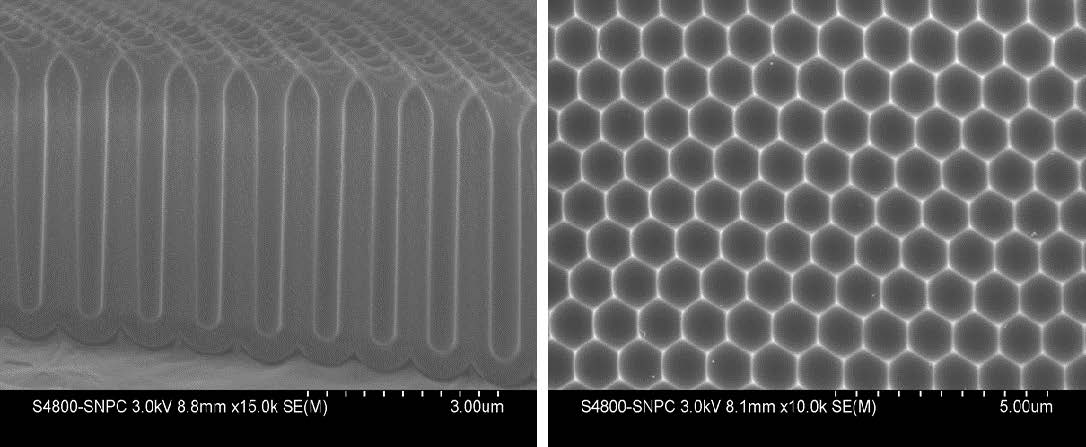
\includegraphics[width=\textwidth]{imgs/Anodization.jpeg}
		
		\caption{Side and bottom morphology of AAO. \cite{lv2017research}}
		\label{fig:Anodization}
	\end{figure}
	
	\subsection{Cleaning Procedure}
	The cleaning of aluminum foils prior to anodization is a critical step to ensure the removal of surface contaminants that could hinder uniform pore formation in anodic aluminum oxide (AAO). Different solvents and techniques are used in sequence to maximize effectiveness.
	
	
	\subsubsection{Solvent Cleaning}
	
	Acetone is a polar aprotic solvent, meaning it has a significant dipole moment (polar) but lacks hydrogen atoms directly bonded to electronegative atoms such as oxygen or nitrogen (aprotic). This absence of hydrogen-bond donors prevents acetone from forming hydrogen bonds, which makes it especially effective at dissolving nonpolar or weakly polar organic residues such as oils, greases, and hydrocarbons.
	
	Isopropyl alcohol (IPA), in contrast, is a polar protic solvent, meaning it is polar and possesses a hydrogen atom bonded to oxygen ($–OH$ group) that can engage in hydrogen bonding. This property allows IPA to effectively dissolve and remove polar contaminants such as salts, ionic residues, water-based impurities, and residual organic films. IPA is also less aggressive than acetone, providing a gentler final cleaning step that reduces the risk of damaging the aluminum surface.
	
	\subsubsection{Sonication}
	
	The cleaning process is further enhanced by ultrasonic bath sonication, typically operated in the frequency range of 20-40 kHz. Sonication generates high-frequency sound waves in the liquid, which induce the formation of microscopic bubbles. These bubbles grow and collapse violently in a process known as cavitation, creating localized zones of high temperature and pressure. The mechanical energy released during cavitation dislodges contaminants from the aluminum surface, including particles trapped in microscopic crevices or surface irregularities. Moreover, cavitation improves the penetration of solvents into fine features, thereby increasing their cleaning efficiency. This combined physical and chemical action ensures a uniform, contaminant-free aluminum surface, which is crucial for consistent anodization and nanostructure formation.
	
	\subsection{Electrochemical Polishing}
	
	Electrochemical polishing (electropolishing) is a process used to produce a smooth, mirror-like aluminum surface by selectively removing microscopic surface irregularities. It also improves surface uniformity at the atomic level, enhances adhesion, increases corrosion resistance, and provides a high-quality substrate for subsequent anodization.
	
	The process relies on anodic dissolution, where aluminum metal at the anode is oxidized under controlled voltage:
	
	\begin{equation}
		\ce{Al_{(metal)} -> Al^3+ + 3 e^-}
		\label{eq:anodic-dissolution}
	\end{equation}
	
	Importantly, this controlled oxidation does not result in the formation of a thick oxide layer. Instead, the electrolyte is designed to chemically dissolve any native \ce{Al_2O_3} as it forms:

	\begin{equation}
		\ce{Al2O3 + 6H+ -> 2Al^3+ + 3H2O}
		\label{eq:oxide-dissolution}
	\end{equation}
	
	This dual mechanism — electrochemical oxidation of aluminum metal and acidic chemical dissolution of aluminum oxide — ensures that the surface is evenly polished rather than roughened by oxide growth.
	
	At the cathode, hydrogen evolution occurs according to the following reaction:

	\begin{equation}
		\ce{2 H^+ + 2 e^- -> H2_{(g)}}
		\label{eq:cathodic-reaction}
	\end{equation}

	The generated \ce{H2_{(g)}} appears as bubbles near the carbon rod at the cathode, indicating the progress of the reduction reaction.
	
	\subsubsection{Electrolyte Composition}
	
	The electrolyte used in this process consists of a mixture of perchloric acid (\ce{HClO4}) and absolute ethanol (\ce{CH3CH2OH}). Perchloric acid serves as a strong oxidizing agent, facilitating anodic dissolution, while simultaneously providing an acidic medium that chemically dissolves aluminum oxide. It also enhances the conductivity of the electrolyte, ensuring uniform current flow across the aluminum surface.
	
	\begin{equation}
		\ce{HCLO4 -> H+ + ClO4-}
		\label{eq:acid-dissociation}
	\end{equation}
	 
	 Ethanol modifies the viscosity of the solution, stabilizes the perchloric acid, and improves wetting of the aluminum surface. It also helps maintain a stable, low-temperature environment, which is crucial because the reaction is highly exothermic and overheating could lead to uncontrolled reactions. Using water instead of ethanol would increase the rate of \ce{Al2O3} formation due to stronger acid dissociation, which is undesirable for achieving a smooth surface. Water has a higher dielectric constant than ethanol, enabling better dissociation of perchloric acid and higher ionic conductivity. However, in electrochemical polishing of aluminum, excessive water content can promote uncontrolled formation of aluminum oxide due to enhanced oxidation reactions at the anode. This oxide layer can passivate the surface and hinder effective polishing. Ethanol, with its lower dielectric constant and reduced water activity, helps limit oxide layer buildup, leading to more uniform surface polishing.
	 
	
	\subsubsection{Process Parameters}
	
	The process parameters, including applied voltage, temperature, and duration, play a critical role in the polishing outcome. Higher voltages accelerate anodic dissolution but risk pitting and uneven material removal, whereas lower voltages slow the process and allow better control. Maintaining a low temperature reduces the reaction rate, minimizes the risk of overheating, and enhances precision, while longer polishing times increase material removal but can lead to over-polishing if excessive. By carefully balancing these factors - for example, applying $14–-15~V$ at $ -0.5\,^\circ C$ for $8$ minutes - the process achieves controlled material removal, smooth surface morphology, and optimal conditions for subsequent anodization.
	
	
	
	\subsection{First Anodization}
	
	Anodization is an electrochemical process in which an oxide layer is formed on the surface of a metal through electrolytic oxidation. For aluminum, the procedure involves immersing high-purity aluminum as the anode and a graphite electrode as the cathode in a suitable electrolyte under controlled operating conditions and an applied voltage \cite{lv2017research}. the
	cathode is a plate or rod composed of a material that is chemically inert
	in the acidic electrolyte (carbon, stainless steel, nickel) \cite{bibideessaa2023review}. Once the current is applied, oxidation takes place at the aluminum surface, leading to the growth of an oxide film, while at the cathode a reduction reaction occurs, accompanied by the evolution of hydrogen gas, as described by\cite{lv2017research}:
	
	\begin{equation}
		\ce{H+ + e- -> 1/2 H2}
		\label{eq:redux}
	\end{equation}
	
	The main anodic reactions can be expressed as:
	
	\begin{equation}
		\ce{2Al + 6OH- -> Al2O3 + 3H2O + 6e-}
		\label{eq:anodic-reactions1}
	\end{equation}
	\begin{equation}
		\ce{4OH- - 4e- -> 2H2O + O2}
		\label{eq:anodic-reactions2}
	\end{equation}
	
	During oxide film formation, the total current consists of both ionic and electronic components. The growth of the oxide layer is primarily governed by ionic current. The behavior of ion conduction differs depending on the electric field strength. Under weak electric fields, diffusion effects become more significant, and ion migration can occur in the opposite direction of the applied field. In contrast, under strong electric fields, ion motion is dominated by the field itself. In the case of anodization, the applied field is extremely intense—on the order of $10^7 \frac{V}{cm}$—so the process is best described as ion transport in a strong electric field\cite{lv2017research}.
	
	Parkhutik and co-workers proposed a steady-state model for pore growth based on experimental observations of current behavior during anodization. According to this model, pore formation proceeds through four distinct stages:
	
	\begin{itemize}
		\item Immediately after the voltage is applied, a compact oxide layer forms on the aluminum surface, with its thickness proportional to the applied voltage (approximately $1.4 \frac{nm}{V}$).
		
		\item Localized dissolution of alumina occurs at certain points within this oxide film, leading to the creation of initial channels. These channels allow oxygen ions to migrate through the barrier layer and react with the underlying metal—this stage is referred to as pore nucleation.
		
		\item During electrolysis, some of these nascent channels continue to expand and compete with one another, eventually developing into deeper and wider pore structures.
		
		\item The system then reaches a steady-state regime in which pores grow in a stable and self-organized manner.
	\end{itemize}
	
	Overall, pore growth involves a balance between two simultaneous processes: the electrochemical formation of oxide at the metal/oxide interface and its dissolution at the oxide/electrolyte interface. This dissolution is enhanced by the strong electric field within the pores and by the action of hydrogen ions present in the electrolyte\cite{lv2017research}.
	
	The anodization of aluminum is typically conducted in strongly acidic environments, with temperature-controlled baths employed to ensure stability and reproducibility of the process. Common electrolytes used for this purpose include phosphoric acid, oxalic acid, and sulfuric acid, each capable of producing porous alumina film structures. These porous films are the most prevalent form of anodic alumina obtained under such conditions. The process is usually carried out at temperatures slightly below or slightly above the freezing point to enhance control over pore formation and prevent localized overheating or burning of the aluminum surface \cite{bibideessaa2023review}.
	
	Alternatively, barrier-type anodic films can be produced using boric acid or organic acid salts, which result in denser oxide layers with higher current density requirements. Among the various acidic electrolytes, oxalic acid, sulfuric acid, and phosphoric acid remain the primary choices for fabricating nanoporous alumina due to their reliability and well-characterized pore formation mechanisms \cite{eessaa2023review}.
	
	In addition to these conventional systems, several studies have reported successful fabrication of nanoporous alumina under atypical conditions—such as at ambient temperature or at temperatures as low as $-40^\circ C$—by employing alkaline electrolytes or mixed-acid systems. More recently, researchers have begun exploring anodization at elevated temperatures as a potential alternative route for nanoporous alumina production. However, the mechanisms governing pore ordering and structure formation at such high temperatures remain insufficiently understood and warrant further systematic investigation \cite{eessaa2023review}.
	
	Anodizing is a surface treatment process widely used to enhance the corrosion resistance of aluminum and its alloys by forming a thick, protective oxide layer. The procedure typically involves several stages, including surface preparation, etching, anodization, and sealing. Different acidic electrolytes—such as sulfuric, chromic, phosphoric, or mixed acids—can be employed to produce anodic films with distinct structural and functional characteristics \cite{eessaa2023review}.
	
	The properties of the anodized layer are strongly influenced by process parameters such as acid concentration, bath temperature, applied voltage, and duration. Higher temperatures and acid concentrations, combined with prolonged anodization, tend to increase oxide dissolution, resulting in more porous film structures. In contrast, anodizing in boric acid forms a dense, nonporous barrier layer, but requires a high voltage (typically $> 400 V$) to achieve a sufficiently thick coating. Sulfuric acid, on the other hand, facilitates porous oxide formation at lower voltages by partially dissolving the barrier layer during oxidation. Consequently, the final film thickness depends more on anodization time than on the applied voltage, often producing oxide layers up to $\sim 100 \mu m$ thick with a dense yet porous morphology \cite{eessaa2023review}.
	
	\subsubsection{Barrier Layer Formation}
	
	Barrier-type anodization produces a compact, nonporous oxide layer that is either insoluble or dissolves much more slowly than it forms. Such layers are typically obtained in neutral or mildly basic electrolytes (pH $> 7$), often containing borate, phosphate, or tartrate salts, and sometimes organic acids like citric, malic, or glycolic acid. Under these conditions, a dense oxide film develops rapidly in response to an applied voltage.
	
	The formation process consists of two main stages. Initially, the current density is held constant while the voltage gradually increases as the oxide thickens, maintaining a steady electric field across the barrier layer. Once the formation voltage is reached, the voltage is kept constant, and further growth proceeds through the migration of \ce{Al^{3+}} ions outward and \ce{O^{2-} / OH- } ions inward. Oxide forms simultaneously at both the metal/oxide and oxide/electrolyte interfaces—approximately $60\%$ at the former and $40\%$ at the latter (Figure \ref{fig:AnodizationOfAAO}).
	
	As the layer thickens, its electrical resistance increases and current decreases until the oxide growth rate equals its dissolution rate. The resulting film is smooth, uniform, and strongly adherent, with a thickness linearly proportional to the applied voltage (typically $1.0 - 1.4 nm V^{-1}$). The barrier layer is hard, wear-resistant, and electrically insulating, providing excellent chemical stability once formation is complete.
	
	\begin{figure}[h!]
		\centering
		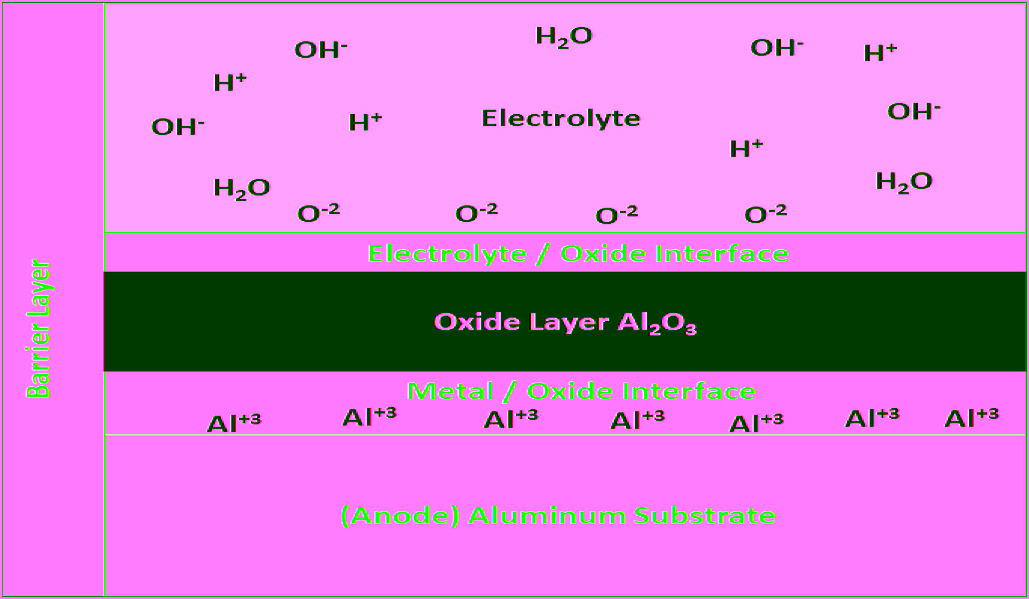
\includegraphics[width=\textwidth]{imgs/anodization of AAO.jpeg}
		
		\caption{Production of barrier layer. \cite{eessaa2023review}}
		\label{fig:AnodizationOfAAO}
	\end{figure}
	
	\subsubsection{Porous Film Formation}
	
	In porous-type anodization, pore formation begins at random sites due to field-assisted dissolution of the oxide at the oxide/electrolyte interface. Initially, oxide growth dominates, but as dissolution increases, the barrier layer thins and pore nucleation occurs. Over time, the process reaches equilibrium, where oxide formation and dissolution proceed at nearly equal rates, resulting in a stable porous structure \cite{eessaa2023review} (Figure \ref{fig:steps}).
	
	Early studies by Wood and Sullivan (1969–1970) revealed that the pores are closely packed and roughly cylindrical, extending perpendicularly from the surface. They also demonstrated that the pore morphology depends strongly on the electrolyte type—such as sulfuric, oxalic, or phosphoric acid. Using advanced microscopy (SEM and TEM), they found that anodic alumina consists of inner and outer layers and that, contrary to earlier assumptions, the oxide is amorphous rather than crystalline. Their refined model established the now widely accepted description of anodic aluminum oxide (AAO) as a self-ordered array of nanoscale tubular pores\cite{eessaa2023review}.
	
	\begin{figure}[h!]
		\centering
		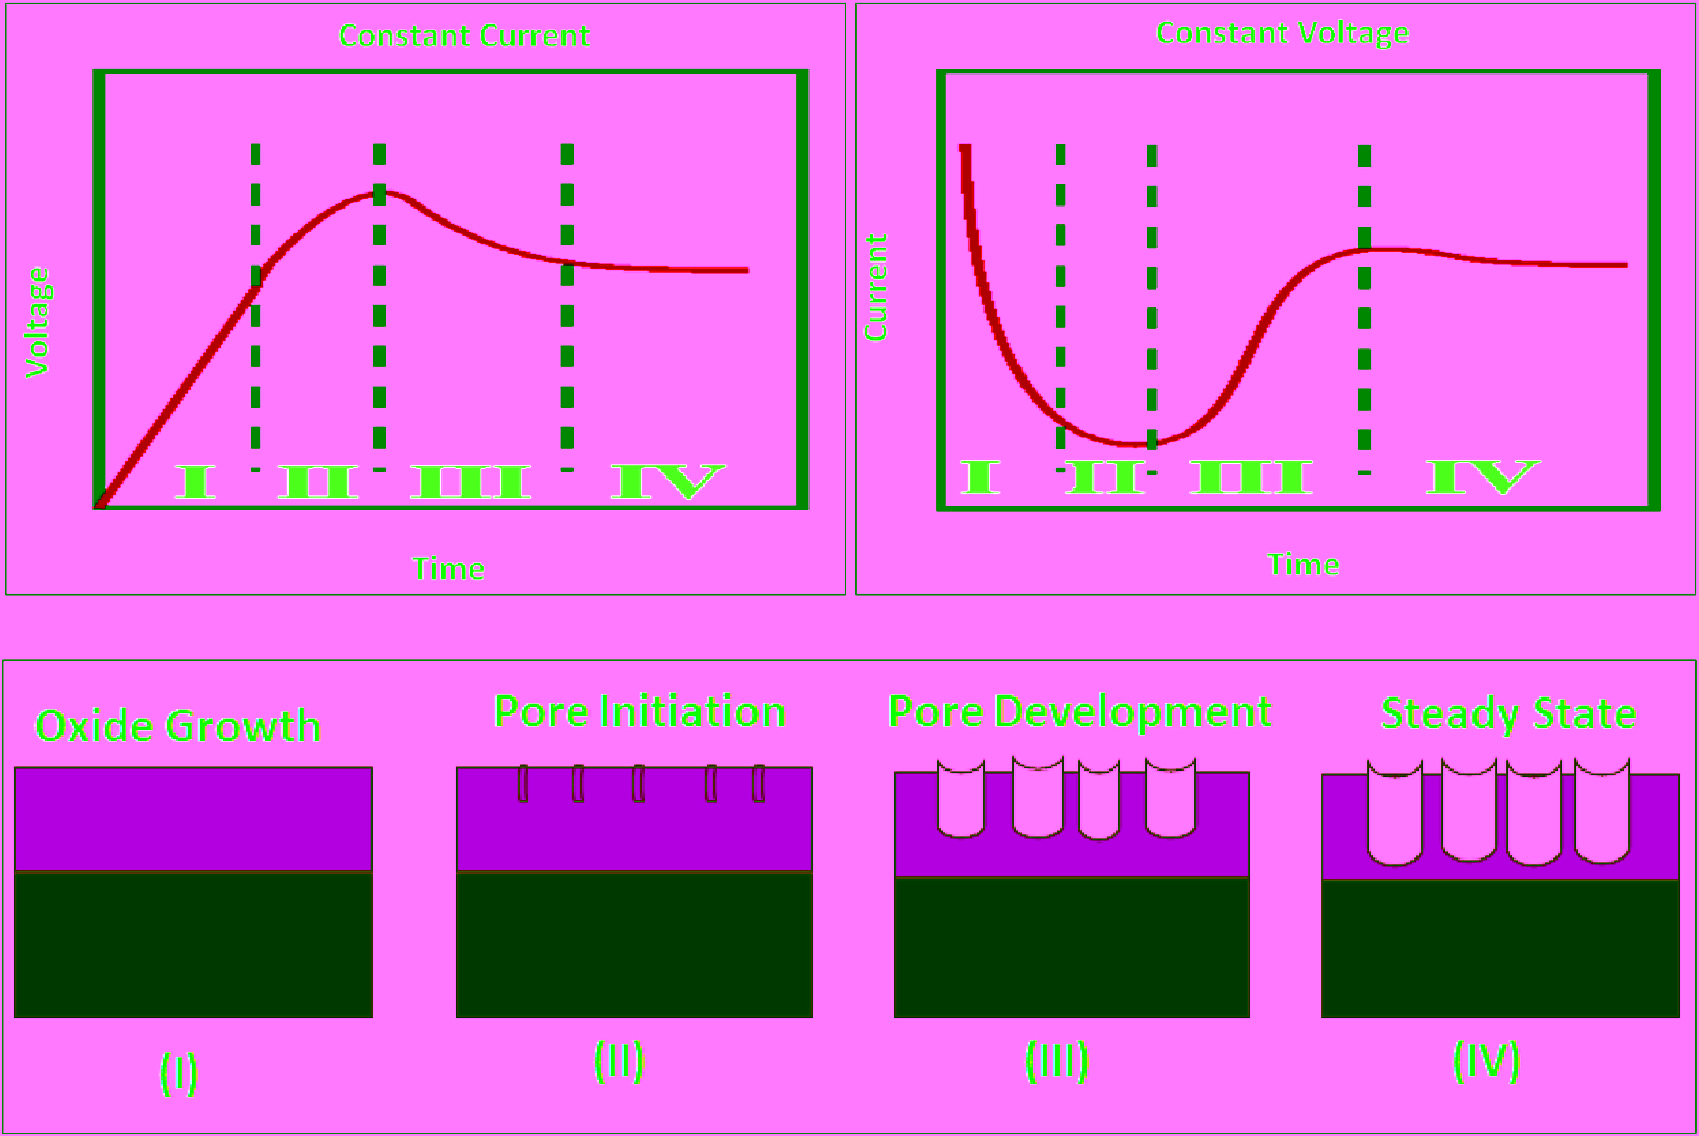
\includegraphics[width=\textwidth]{imgs/steps.jpeg}
		
		\caption{Pores formation steps. \cite{eessaa2023review}}
		\label{fig:steps}
	\end{figure}
	
	The anodic oxide layer consists of two distinguishable regions: an inner monolithic layer and an outer porous layer. The inner layer is continuous and uniform, without visible cell boundaries, so it does not exhibit a polygonal shape. In contrast, the outer layer contains cylindrical pores that can be observed using electron microscopy. Individually, these pores are cylindrical, but their arrangement forms an ordered pattern.
	
	The overall cell structure is defined by the pore arrangement. If one connects the centers of adjacent pores, a hexagonal lattice emerges, reflecting the close packing of the pores (HCP). To define the cell walls, a Wigner–Seitz construction can be applied around each pore, producing a hexagonal boundary that represents the effective unit cell surrounding the pore. Thus, while the inner layer is monolithic and the pores themselves are cylindrical, the combination of pore packing and Wigner–Seitz analysis naturally gives rise to hexagonal cells (Figure \ref{fig:cell}).
	
	\begin{figure}[h!]
		\centering
		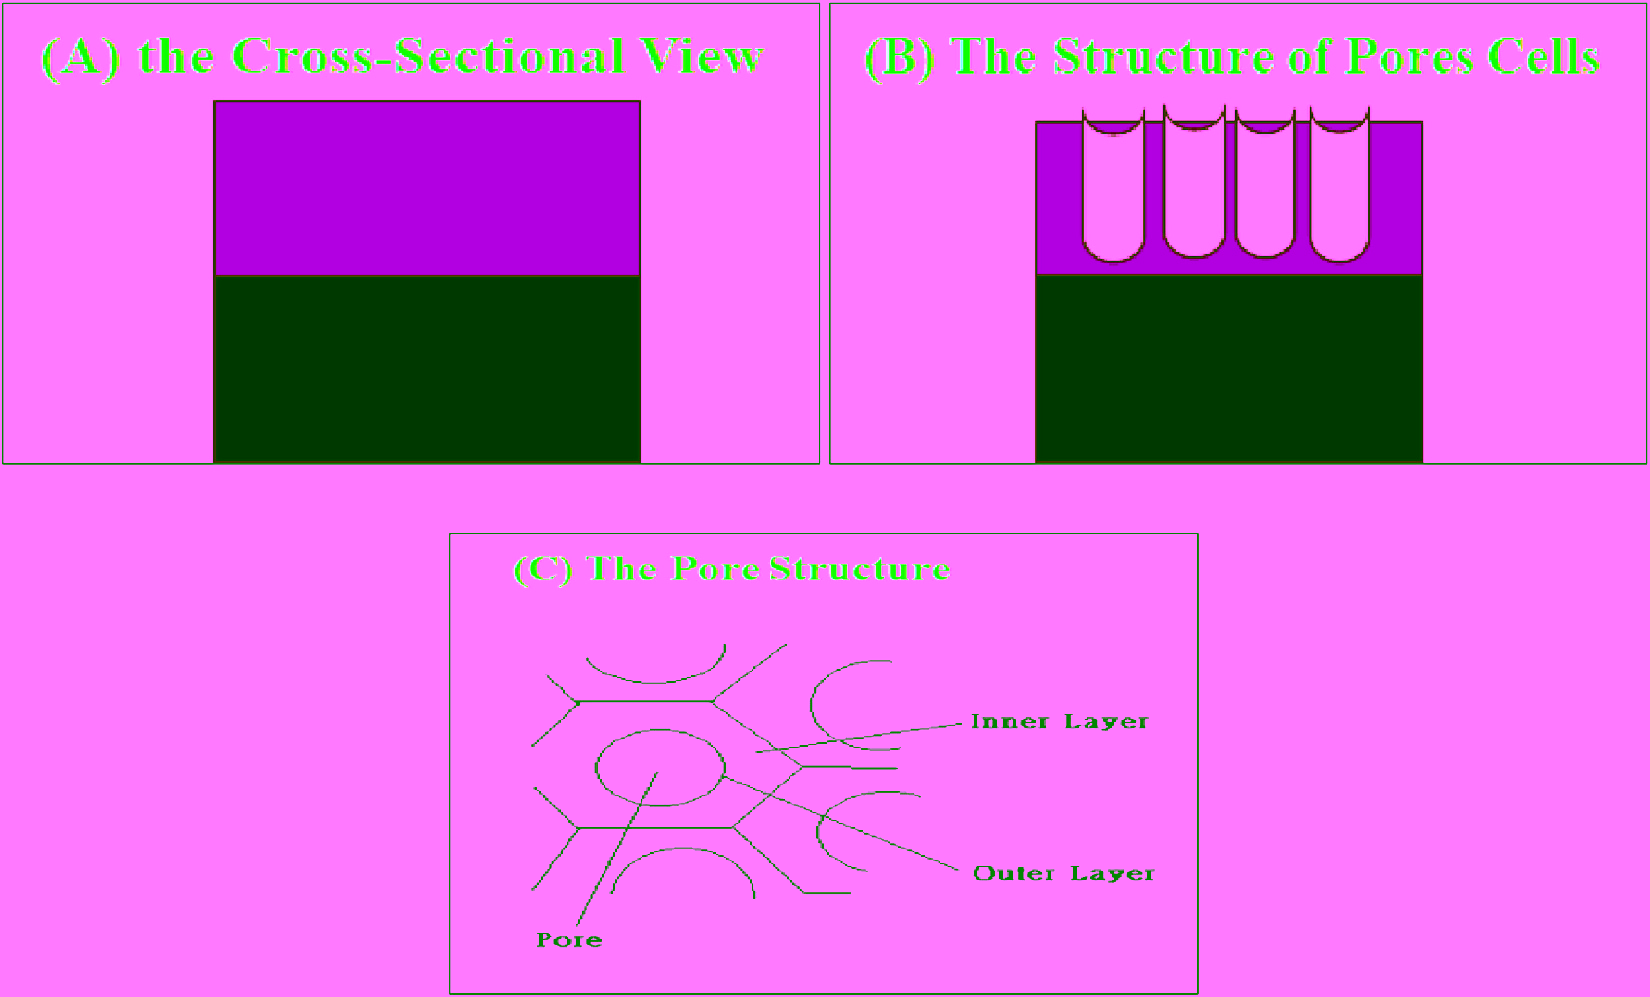
\includegraphics[width=\textwidth]{imgs/cell.jpeg}
		
		\caption{Pores formation steps. \cite{eessaa2023review}}
		\label{fig:cell}
	\end{figure}
	
	The pores in anodic aluminum oxide (AAO) naturally form a hexagonal close-packed (HCP) lattice due to a combination of electrochemical, mechanical, and geometric factors. Pore formation is driven by the local electric field at the oxide/electrolyte interface, and new pores tend to nucleate where the field is strongest. Existing pores create a repulsive effect, so the spacing between pores becomes uniform, leading to a self-organized pattern.
	
	Additionally, the growing oxide layer experiences mechanical stress, and a hexagonal arrangement allows each pore to be equidistant from its neighbors, minimizing elastic stress in the surrounding material. Hexagonal packing is also the most efficient way to arrange circular pores on a plane, maximizing pore density while maintaining uniform spacing. The combination of these effects results in the energetically favorable and stable HCP lattice observed in AAO films.
	
	Modern studies have enabled the fabrication of controllable pore arrays using AAO templates for nanomaterial growth. However, producing a perfect AAO template remains challenging. Key factors influencing template quality include the type of electrolyte, applied voltage, anodization time, temperature, and other minor parameters (Table \ref{tab:nanopores} ). Each electrolyte must be used at an appropriate voltage to balance oxide growth and dissolution, forming the characteristic porous structure. The resulting oxide layer can exceed $100 \mu m$ in thickness, with about $40\%$ penetrating below the original metal surface. Pore density is typically very high, ranging from $30 - 60 \times 10^{10} ~ \frac{cells}{in^2}$ \cite{eessaa2023review}.
	
	\begin{table}[h!]
		\centering
		\caption{The diameter and density of nanopores \cite{YANG2003440}.}
		\begin{tabular}{lccc}
			\toprule
			\textbf{Acidic medium} & \textbf{H$_2$SO$_4$} & \textbf{(COOH)$_2$} & \textbf{H$_3$PO$_4$} \\
			\midrule
			Voltage (V) & 60 & 28 & 140 \\
			Distance between neighboring pore centers (nm) & 150 & 65 & 400 \\
			Diameter of nanopores (nm) & 70 & 35 & 120 \\
			\bottomrule
		\end{tabular}
		\label{tab:nanopores}
	\end{table}
	
	
	The formation of the nanoporous oxide layer produces a self-organized hexagonal pore array, as documented in several studies. Unlike the barrier layer, this structure consists of a thin, non-porous oxide layer next to the metal substrate that continuously regenerates at the pore base while the pore walls grow over time. Pore size and spacing are primarily determined by the electrolyte type and concentration, anodic voltage, and bath temperature. Typical electrolytes are acidic (pH $< 5$), such as sulfuric, phosphoric, and oxalic acids, or combinations of inorganic and organic acids (Table \ref{tab:nanopores}). Lower-concentration acids produce thicker, harder, and less porous coatings, while higher-concentration acids yield more porous layers. The most critical factor in forming the porous oxide is the electrolyte’s ability to sustain \ce{Al^{3+}} ion flow from the metal substrate. \ce{Al^{3+}} ions are lost either through direct field-assisted ejection or oxide layer dissolution, with accelerated (field-assisted) dissolution occurring in regions of high current \cite{eessaa2023review}.
	
	The steady-state growth of the porous oxide layer results from a balance between field-enhanced oxide dissolution at the oxide/electrolyte interface at the pore base and oxide formation at the metal/oxide interface due to migration of \ce{O^{2-}} and \ce{OH^-} ions (Figure \ref{fig:ionFlow}). Pore diameter depends on the anodizing voltage, while the electric field in the pore walls is insufficient to drive ion migration. Oxidation occurs perpendicular to the surface, forming columnar walls with a central channel that extends from the pore base to the oxide surface. Volumetric expansion during oxidation (factor $\sim$2) and mechanical stresses from neighboring pores contribute to wall growth; experimental expansion factors range from 0.8 to 1.6 depending on electrolyte, concentration, and voltage \cite{eessaa2023review}.  
	
	The porous layer mainly consists of amorphous \ce{Al2O3}, electrolyte anions (up to 20\%), small amounts of water, and nanocrystallites. Voids may form due to oxygen evolution or defects in the barrier layer. Anodization conditions can yield either amorphous or crystalline oxide structures, as confirmed by XRD studies using oxalic acid electrolytes \cite{eessaa2023review}.  
	
	Mechanical stress at the metal/oxide interface also influences self-ordering of the pores. Initially, pores form randomly, but with continued anodization they self-adjust into a uniform hexagonal array with identical pore sizes. Pore density can vary from $10^8$ to $10^{12}$ cm$^{-2}$ depending on fabrication parameters \cite{eessaa2023review}.
	
	\begin{figure}[h!]
		\centering
		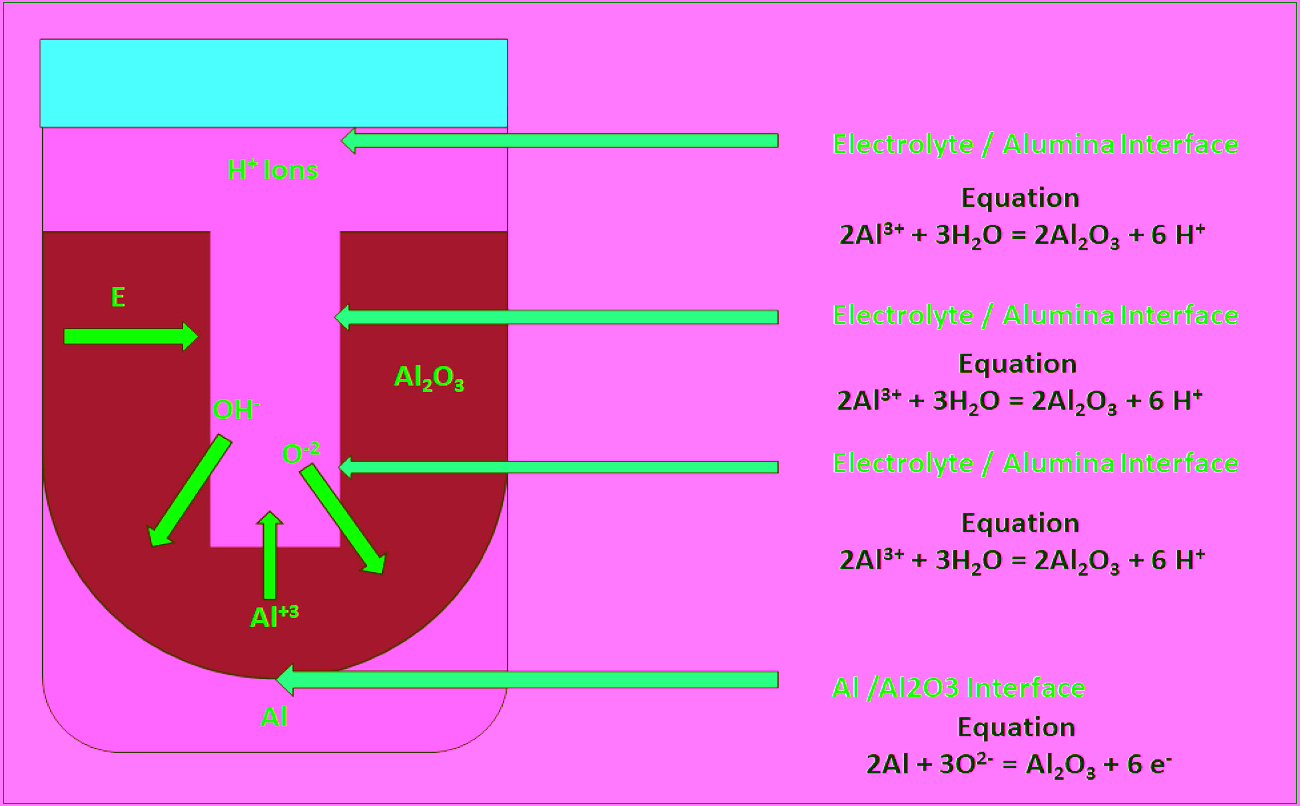
\includegraphics[width=\textwidth]{imgs/ionFlow.jpeg}
		
		\caption{The flow of ions during the formation of pores. \cite{eessaa2023review}}
		\label{fig:ionFlow}
	\end{figure}
	
	
	
	\subsubsection{Factors Affecting the Anodizing Process}
	
	The formation of anodic alumina is governed by several parameters, including the electrolyte composition, anodizing voltage, duration, and temperature. Among these, the electrolyte plays the most critical role in determining whether the oxide layer develops as a porous or barrier type. Non-acidic electrolytes generally do not dissolve the barrier oxide, or do so much more slowly than the rate of oxide formation, leading to the growth of an amorphous, compact protective layer on the aluminum surface (Table \ref{tab:basic}). In contrast, acidic electrolytes promote the continuous dissolution and regeneration of alumina, which drives the self-organization of pores \cite{eessaa2023review}.
	
	
	\begin{table}[h]
		\caption{A collection of inert electrolytes that are used in the manufacture of barrier layers \cite{talbot2018corrosion}.}
		\begin{tabular}{|l|l|c|c|}
			\hline
			\textbf{Non-Acid} & \textbf{Equation} & \textbf{Conc., (M)} & \textbf{pH} \\ \hline
			Ammonium Adipate & NH$_2$OCO(CH$_2$)$_4$COONH$_4$ & 150 g/L & 6.4 \\ \hline
			Sodium Borate & Na$_2$B$_4$O$_7$ & 2.2 & 7 \\ \hline
			Sodium chromate & Na$_2$CrO$_4$ & 0.1 & 10 \\ \hline
			Sodium hydrogen phosphate & Na$_2$HPO$_4$ & 0.1 & 9.4 \\ \hline
			Sodium hydroxide & NaOH & 0.01, 0.03 \& 0.1 & Not specified \\ \hline
			Sodium sulfate & Na$_2$SO$_4$ & 0.1 & 5.8 \\ \hline
		\end{tabular}
		\label{tab:basic}
	\end{table}
	
	
	The type and concentration of acid directly influence the pore diameter, ordering, and morphology. For example, anodization in $0.35~M$ oxalic acid results in pores of approximately $100~nm$, while $0.3~M$ sulfuric acid produces smaller pores of around $40~nm$. This difference originates from the pH and dissolution dynamics of the acids. Oxalic acid, having a higher pH than sulfuric acid, is less aggressive, resulting in slower dissolution and thus larger pores. Conversely, sulfuric acid, being more acidic, provides a higher concentration of anions that enhance the horizontal dissolution rate of alumina, leading to smaller but more uniformly distributed pores \cite{eessaa2023review}.
	
	The electric field applied during anodization also affects ion transport and dissolution kinetics. A stronger field accelerates the migration of \ce{Al^{3+}}, \ce{O^{2-}}, and \ce{OH^-} ions, enhancing field-assisted dissolution at the oxide/electrolyte interface. This process balances oxide growth at the metal/oxide interface, defining the final pore geometry. The dissolution rate in the lateral direction is typically higher than in the vertical direction, particularly in sulfuric acid, resulting in more compact pore arrays with higher ordering. This correlation between smaller pore diameter and higher array regularity has been experimentally verified \cite{eessaa2023review}. 
	
	For practical applications, sulfuric acid is often preferred for producing highly ordered and densely packed nanopores, while oxalic and phosphoric acids are used when larger pores ($10 - 240~nm$) are desired. These electrolytes remain the most widely used in the fabrication of anodic aluminum oxide (AAO) templates (Tables~\ref{tab:acids} and~\ref{tab:acidVolt}) \cite{eessaa2023review}.
	

	\begin{table}[h]
		\caption{The primary acids that make up the various kinds of electrolytes are often used in the process of producing a porous oxide layer on an aluminum substrate.}
		\renewcommand\theadfont{\bfseries} % Makes headers bold
		\begin{tabular}{|l|l|c|c|}
			\hline
			\thead{Main Acid\\ used in\\ Electrolyte} & \thead{Molecular\\ Formula} & \thead{Concentration\\ (M)} & \thead{Pore Size\\ Range (nm)} \\ \hline
			Acetic & CH$_3$CO$_2$H & 1 & Not specified \\ \hline
			Citric & HOOCCH$_2$(CO$_2$H) & 0.1 to 2 & 90 to 250 \\ \hline
			Chromic & H$_2$CrO$_4$ & 0.3, 0.44 & 17 to 100 \\ \hline
			Glycolic & CH$_2$(OH)COH & 1.3 & 35 \\ \hline
			Malic & HO$_2$CCH$_2$CH(OH) & 0.15 to 0.3 & Not specified \\ \hline
			Malonic & CO$_2$H(CO$_2$H)$_2$ & 0.1 to 5 & Not specified \\ \hline
			Oxalic & C$_2$H$_2$O$_4$ & 0.2 to 0.5 & 20 to 80 \\ \hline
			Phosphoric & H$_3$PO$_4$ & 0.04 to 1.1 & 30 to 235 \\ \hline
			Sulfuric & H$_2$SO$_4$ & 0.18 to 2.5 & 12 to 100 \\ \hline
			Tartaric & CH(OH)(COOH)CH(OH)COOH & 0.1 to 3 & Not specified \\ \hline
		\end{tabular}
		\label{tab:acids}
	\end{table}
	
	
	\begin{table}[h]
		\caption{To build a porous oxide layer on an aluminum substrate, the voltage, and times for three regularly used electrolytes are as follows.}
		\begin{tabular}{|l|c|c|c|c|}
			\hline
			\textbf{Acid} & \textbf{Conc., (M)} & \textbf{Voltage, (Volts)} & \textbf{Pore Size, (nm)} & \textbf{Time, (hours)} \\ \hline
			\multirow{10}{*}{Oxalic} & 0.25 & 60 & 75 & 8,8 \\ \cline{2-5}
			& 0.3 & 40 & Not specified & variable \\ \cline{2-5}
			& 0.3 & 40 & 80 & 8, variable \\ \cline{2-5}
			& 0.3 & 40 & 50 & 10,5 min \\ \cline{2-5}
			& 0.3 & 60 & 80 & 3,8 \\ \cline{2-5}
			& 0.3 & 40 & 40-50 & 40 min, 2 \\ \cline{2-5}
			& 0.3 & 40, 50 & 20, 35 & variable \\ \cline{2-5}
			& 0.3 & 30 & 40 & 8,10 \\ \cline{2-5}
			& 0.4 & 40 & 50 & 8,10 \\ \cline{2-5}
			& 0.5 & 50 & 80 & 8,10 \\ \cline{2-5}
			& 0.3 & 40 & 22 & 12, 4, 8, 12 \& 16 \\ \cline{2-5}
			& Not specified & 195 & 200 & variable \\ \hline
			\multirow{6}{*}{Phosphoric} & 0.4 & 5 to 40 & 20 to 75 & 1 step/variable \\ \cline{2-5}
			& 0.4 & 80 & 80 & 1 step \\ \cline{2-5}
			& 0.42 & 87 to 117 & 64 to 79 & 1 step/variable \\ \cline{2-5}
			& 0.5 & 18 & 70 & 4, variable \\ \cline{2-5}
			& 2.4 & 15 to 25 & 13 to 27 & 2-step/ variable \\ \hline
			\multirow{3}{*}{Sulfuric} & Not specified & 12, 25, 40 & 25, 50, 100 & Not specified \\ \cline{2-5}
			& 0.3 & 25 & 20 & 12, 4, 8, 12 \& 16 \\ \hline
		\end{tabular}
		\label{tab:acidVolt}
	\end{table}
	
	
	The anodizing voltage is a critical parameter that must be optimized for each acid electrolyte and its concentration. Exceeding the suitable voltage range can lead to dielectric breakdown of the oxide barrier layer, resulting in local burning and irregular pore formation. This breakdown arises mainly from three factors: (1) localized heating that increases conductivity at the pore bases, (2) field-induced ionization of atoms that generates excess electrons, and (3) pre-existing microcracks that facilitate oxide rupture. The relative conductivity of common anodizing acids follows the order \ce{H2SO4} > (COOH)$_2$ > \ce{H3PO4}, corresponding to typical anodizing voltage ranges of $5 - 40~V$ for sulfuric acid, $30 - 140~V$ for oxalic acid, and $80 - 200~V$ for phosphoric acid \cite{eessaa2023review}.  
	
	Alaba \textit{et al.} demonstrated that nanoporous alumina can be fabricated using a single-step anodization method without removing the initial oxide layer, employing $20\%$ phosphoric acid at $60~V$ and temperatures between $30 - 38^{\circ}C$. This relatively high acid concentration produced uniform pores of $80–120~nm$ in diameter at room temperature. Similarly, Chung \textit{et al.} investigated the effect of voltage mode and temperature on pore morphology during one-step anodization in $0.5~M$ oxalic acid. Two voltage regimes were compared: direct current anodization (DCA) and hybrid pulse anodization (HPA), conducted at $5 - 15^{\circ}C$. HPA, which alternates between high and low voltages, provides improved heat dissipation, resulting in more uniform and circular pore structures compared to DCA. Higher temperatures, however, accelerate oxide growth and increase pore size \cite{eessaa2023review}.  
	
	Conventional AAO templates are typically fabricated using two-step DCA at low temperatures ($0 - 5^{\circ}C$) to minimize chemical dissolution, though this approach is relatively time-consuming. In contrast, pulse anodization (PA) and hybrid pulse anodization (HPA) methods—employing alternating positive and small negative voltages—offer enhanced control over pore structure, reduced processing time, and improved mechanical and corrosion resistance. These recent developments suggest that voltage modulation techniques such as HPA can achieve high-quality AAO films more efficiently than traditional DCA \cite{eessaa2023review}.
	
	The anodization duration determines the final thickness of the AAO film, which directly influences pore ordering. Thicker AAO layers generally exhibit greater variation in pore diameter. For instance, when anodized in oxalic acid, a 3~h process yields a thickness of about $50~\mu m$, whereas 10~h of anodization produces approximately $45~\mu m$ with improved pore regularity. However, excessively long anodization deteriorates film quality due to chemical dissolution and structural fatigue. In practice, anodizing beyond the optimal duration (e.g., 12~h instead of 8~h) results in severe surface damage and partial dissolution of the aluminum substrate \cite{jessensky1998self}.  
	
	Temperature is not a dominant parameter in determining pore morphology, but it strongly affects current stability. Heat generated during anodization can cause current fluctuations and disrupt pore growth; therefore, the process should be maintained at low temperatures ($1 - 3^{\circ}C$) to facilitate heat dissipation. The extent of heat generation depends on the electrolyte type, with sulfuric acid producing more exothermic reactions than oxalic acid~\cite{jessensky1998self}.  
	
	Araoyinbo \textit{et al.} reported that increasing the anodizing voltage enhances current density and significantly enlarges pore diameter from $\sim 40~nm$ to $300~nm$, accompanied by minor structural phase changes in the aluminum substrate (from FCC to monoclinic near $39^{\circ}C$ and $45^{\circ}C$). The degree of pore ordering was found to depend strongly on both anodizing voltage and duration. At the metal/oxide interface, pores are typically smaller and more uniformly arranged than those at the oxide/electrolyte boundary, where spacing increases \cite{eessaa2023review}.  
	
	Further comparison of anodization in $0.3~M$ oxalic and sulfuric acids showed that well-ordered nanopore arrays with uniform diameters can form under moderate and stable current densities. Conversely, low current densities yield disordered arrangements, while excessively high or unstable currents cause irregular pore sizes and disrupted ordering. These results highlight that both anodizing voltage and the corresponding current density play decisive roles in achieving self-ordered nanoporous alumina (PAA) \cite{eessaa2023review}.
	
	\subsection{Etching Away the First Anodized Layer}
	
	Following the first anodization, the aluminum surface becomes covered with a porous alumina (\ce{Al2O3}) layer that is typically irregular due to nonuniform pore nucleation and the presence of surface defects on the pre-polished substrate. To achieve a more ordered porous structure in the subsequent anodization, this initial oxide layer is selectively removed through a chemical etching process. The etching not only eliminates the disordered alumina but also exposes a textured aluminum surface characterized by a periodic pattern of concave dimples or scallops corresponding to the base of the previously formed pores. These ordered concavities serve as preferential nucleation sites during the second anodization, guiding the formation of a highly uniform and hexagonally arranged pore array \cite{gu20163d}.
	
	The etching solution typically consists of a mixture of phosphoric acid (\ce{H3PO4}) and chromic acid (\ce{H2CrO4}), often prepared by dissolving chromium trioxide (\ce{CrO3}) in the phosphoric acid medium. This mixture offers a highly selective etching environment that efficiently dissolves alumina while leaving the underlying metallic aluminum largely intact. The phosphoric acid contributes primarily to the chemical dissolution of \ce{Al2O3} through proton attack according to the following reaction:
	
	\begin{equation}
		\ce{Al2O3 + 6H+ -> 2Al^{3+} + 3H2O}
		\label{eq:Al2O3Dissolution}
	\end{equation}
	
	Here, \ce{H3PO4} dissociates to produce \ce{H+} and \ce{H2PO4-}, which aid in breaking the Al–O bonds in the oxide layer. The mild etching action of phosphoric acid also smooths the aluminum surface, while simultaneously enhancing the oxidative power of the chromic component.
	
	The role of \ce{CrO3}, on the other hand, is primarily oxidative. In aqueous environments, \ce{CrO3} forms chromic acid (\ce{H2CrO4}), which dissociates to yield reactive species such as \ce{H+} and \ce{HCrO4-}:
	
	\begin{equation}
		\ce{CrO3 + H2O -> H2CrO4 -> H+ + HCrO4^-}
		\label{eq:chromicAcidFormation}
	\end{equation}
	
	These species act as strong oxidizers, facilitating the conversion of any exposed metallic aluminum into a thin, passivating chromium-rich oxide layer. This selective passivation prevents excessive attack on the aluminum substrate, ensuring that only the alumina film is dissolved. The synergistic action of \ce{H3PO4} and \ce{CrO3} thus achieves controlled removal of the oxide while preserving the prepatterned texture essential for pore ordering.
	
	Maintaining the etching bath at a high temperature ($ \approx 98~^{\circ}C$) greatly accelerates the dissolution kinetics of alumina and enhances the reactivity of both acids, leading to a cleaner and more uniform surface. The combination of thermal activation, selective oxidation, and controlled chemical dissolution ensures that the etched aluminum surface provides an ideal foundation for the second anodization, where a self-ordered nanoporous alumina film with improved uniformity and long-range order is subsequently formed.
	
	
	\subsection{Barrier Layer Thinning}
	
	During the anodization of aluminum, a thin, compact oxide layer known as the barrier layer forms at the interface between the aluminum substrate and the porous anodic alumina (PAA). This layer, typically a few to several tens of nanometers thick depending on the anodization voltage, is electrically insulating and prevents direct charge transfer between the aluminum and any material within the pores. For subsequent processes such as metal electrodeposition or electrical contacting, this barrier must be thinned or partially removed to enable efficient electron transport \cite{gu20163d}.
	
	The barrier thinning process relies on the principle of field-assisted oxide dissolution. When the anodization voltage is gradually reduced in an acidic electrolyte, the electric field across the barrier layer decreases, leading to a situation where the rate of oxide dissolution at the pore bottoms exceeds its growth rate. As a result, the barrier thickness continuously decreases until it reaches a few nanometers. The reduction must be controlled carefully to maintain uniform thinning across the entire template and avoid dielectric breakdown or pore collapse (Figure \ref{fig:thin}) \cite{gu20163d}.
	
	When the barrier layer becomes sufficiently thin—typically around 4 nm—it allows quantum tunneling of electrons through the oxide. This tunneling effect is essential for enabling electrochemical deposition of metals inside the pores and establishing electrical continuity with the underlying aluminum substrate. However, if the barrier is thinned excessively, it may lose its integrity, leading to nonuniform current distribution or short-circuiting between pores. Therefore, an optimal balance is required: the barrier must be thin enough to permit electron tunneling, yet stable enough to preserve structural order and uniformity across the anodic template \cite{gu20163d}.
	
	\begin{figure}[htpb]
		\centering
		\includegraphics[width=\textwidth]{imgs/thin.jpg}
		
		\caption{Barrier Thinning Concept}
		\label{fig:thin}
	\end{figure}
	
	\subsection{Pb Electrodeposition}
	Electrodeposition is an electrochemical process in which metal ions in an electrolyte are reduced and deposited as a solid metal layer on a conductive substrate under the influence of an external electric field. In the context of porous anodic alumina (PAA) templates, electrodeposition enables the precise filling of nanochannels or the formation of metallic nanoclusters at the pore bottoms, which can later serve as active components or electrical contacts in nanoelectronic devices.
	
	Following barrier layer thinning, the aluminum substrate beneath the pores becomes sufficiently conductive to allow electron tunneling through the thin oxide barrier. This enables localized electrochemical reactions to occur at the pore bases during deposition. Lead ions (\ce{Pb^{2+}} in the electrolyte are reduced to metallic lead (\ce{Pb}) through the cathodic reaction:
	
	\begin{equation}
		\ce{Pb^{2+} + 2e -> Pb(s)}
		\label{eq:PbCathode}
	\end{equation}
	
	The reverse anodic process, in which metallic lead is reoxidized, can also occur under alternating electrical conditions.
	
	In this work, an alternating current (AC) method was employed instead of conventional direct current (DC) deposition. The use of AC is advantageous in nanoporous systems because it allows charge balancing within the confined geometry of the pores, mitigates the buildup of space charge and concentration gradients, and promotes uniform nucleation and growth of nanoclusters at the pore bases. The alternating potential periodically reverses the electrode polarity, which assists in removing loosely bound ions or byproducts from the pore openings, thereby maintaining stable deposition kinetics \cite{gu20163d}.
	
	Additionally, the presence of trisodium citrate ( \ce{Na3C6H5O7}) in the electrolyte acts as a complexing agent for lead ions, forming soluble \ce{Pb}–citrate complexes that stabilize the ionic concentration and reduce the likelihood of premature precipitation of \ce{Pb(OH)2} or other lead salts. This complexation ensures controlled release of \ce{Pb^{2+}}
	during the reduction phase, leading to smoother and more uniform metal growth.
	
	Overall, this process enables the formation of a thin, continuous layer of metallic lead at the pore bottoms. The deposited Pb layer serves as an essential electrical contact and can also influence subsequent device performance by improving charge transport across the PAA–metal interface.
	
	
	%------------- Commandes utiles ----------------
	
	\section{Methodology}
	
	
	
	\subsection{Introduction}
	
	This section describes the complete methodology employed for the fabrication, structural characterization, and photoelectrical evaluation of perovskite nanowire photodetectors. The overall experimental workflow involves the preparation of a porous anodic alumina (PAA) template, the infiltration or vapor-phase growth of perovskite nanowires within the template, and the subsequent device assembly and testing. Two distinct fabrication approaches were utilized—spin coating and chemical vapor deposition (CVD)—to comparatively investigate their influence on nanowire morphology, uniformity, and device performance.
	
	The PAA template serves as a self-organized, hexagonally ordered scaffold that defines the nanowire geometry and ensures vertical alignment during growth. In the spin-coating method, a perovskite precursor solution is infiltrated into the PAA pores under controlled conditions, followed by thermal annealing to form uniform, confined nanowire arrays. In contrast, the CVD technique relies on vapor-phase transport and condensation of the perovskite precursor, offering a solvent-free route with potentially higher crystallinity and improved environmental stability.
	
	Following nanowire formation, an indium tin oxide (ITO) electrode was deposited by sputtering to complete the photodetector device structure. The devices were then subjected to systematic structural, morphological, and optoelectronic characterization to assess the effects of fabrication parameters on their photoresponse and overall performance. This methodological framework enables a direct comparison between the spin-coated and CVD-grown perovskite nanowires, clarifying the correlation between processing route, structure, and functionality.
	
	
	\subsection{Perovskite Photo Detector Fabrication}
	
	\subsubsection{Aluminum Chip Preparation}
	In the first step, aluminum foils with a thickness of $250 \mu m$ were cut into chips of dimensions $3\times 4 cm^2$. The chips were then flattened by sandwiching them between glass slides and applying pressure using a mechanical press to ensure uniform thickness.
	
	After flattening, the aluminum chips were cleaned to remove surface contaminants such as oils, dust, and native residues. The cleaning procedure consisted of sequential bath sonication: 5 minutes in acetone followed by 5 minutes in isopropyl alcohol (IPA). This process ensured that the chips were free of organic and particulate impurities, preparing them for subsequent anodization. 
	
	\subsubsection{Electrochemical Polishing}
	
	
	In this step, electrochemical polishing was performed to smooth the aluminum surface and prepare it for uniform anodization in subsequent steps. The process was carried out using a standard electrochemical cell, with an acidic electrolyte composed of $25\%~v/v~\text{perchloric acid}(HClO_4)$ and $75\%~v/v~\text{absolute ethanol} (CH_3CH_2OH)$. The aluminum chips served as the anode, while a suitable counter electrode (e.g., carbon rod) completed the circuit. Polishing was performed for 8 minutes under an applied voltage of $14–-15~V$ at a temperature of approximately $-0.5\,^\circ\text{C}$. This treatment reduces surface roughness, removes residual mechanical defects, and promotes the formation of highly ordered nanopores during the anodization step.
	
	\begin{figure}[htpb]
		\centering
		% Panel (a)
		\begin{subfigure}[b]{0.45\textwidth}
			\centering
			\includegraphics[width=\textwidth]{imgs/EP solution.jpg}
			\caption{Electrochemical Polishing Solution}
			\label{fig:EPs}
		\end{subfigure}
		\hfill
		% Panel (b)
		\begin{subfigure}[b]{0.45\textwidth}
			\centering
			\includegraphics[width=\textwidth]{imgs/EP cell.jpg}
			\caption{Electrochemical cell used for Electrochemical Polishing}
			\label{fig:EPc}
		\end{subfigure}
		
		\vspace{0.3cm} % optional spacing between rows
		
		% Panel (c)
		\begin{subfigure}[b]{0.45\textwidth}
			\centering
			\includegraphics[width=\textwidth,angle=-90]{imgs/done EP.jpg}
			\caption{Electrochemical Polished Aluminum Chip}
			\label{fig:EPDone}
		\end{subfigure}
		
		\caption{Step-by-step Electrochemical Polishing process.}
		\label{fig:EP}
	\end{figure}
	
	\subsubsection{First Anodization}
	\label{sec:FirstAnodization}
	
	The first anodization was carried out in a mixed electrolyte consisting of deionized water, ethylene glycol, and phosphoric acid (\ce{H3PO4}) in a volumetric ratio of $200:100:1$. To prepare one liter of electrolyte, $600~mL$ of deionized water and $300~mL$ of ethylene glycol were combined in a clean bottle, followed by the addition of $3 mL$ of phosphoric acid using a pipette. The solution was stirred for one hour at moderately high speed to ensure complete homogenization before use.
	
	Electropolished aluminum chips were then placed together in a container filled with the prepared electrolyte. The chips were connected to the positive terminal of a DC power supply, serving as the anode, while a carbon rod connected to the negative terminal served as the cathode. The electrochemical cell was placed in a chiller and maintained at $-1\, ^\circ C$ throughout the process in order to suppress excessive heating and maintain stable anodization conditions. Temperature control is critical, as anodization performed at higher temperatures, such as room temperature, can lead to localized burning of the aluminum surface. This manifests either as the formation of dark spots or as non-uniform current pathways, both of which prevent the uniform development of nanopores.
	
	The anodization procedure was initiated in current-controlled mode, applying a total current of $32~mA$ (corresponding to $8~mA$ per chip for four chips). The voltage was allowed to rise until it reached $200~V$, after which the system was switched to voltage-controlled mode by increasing the maximum current limit. The anodization was continued under these conditions for $30$ minutes, ensuring uniform pore initiation and growth across the aluminum chip surfaces.
	
	
	\begin{figure}[htpb]
		\centering
		% Panel (a)
		\begin{subfigure}[b]{0.45\textwidth}
			\centering
			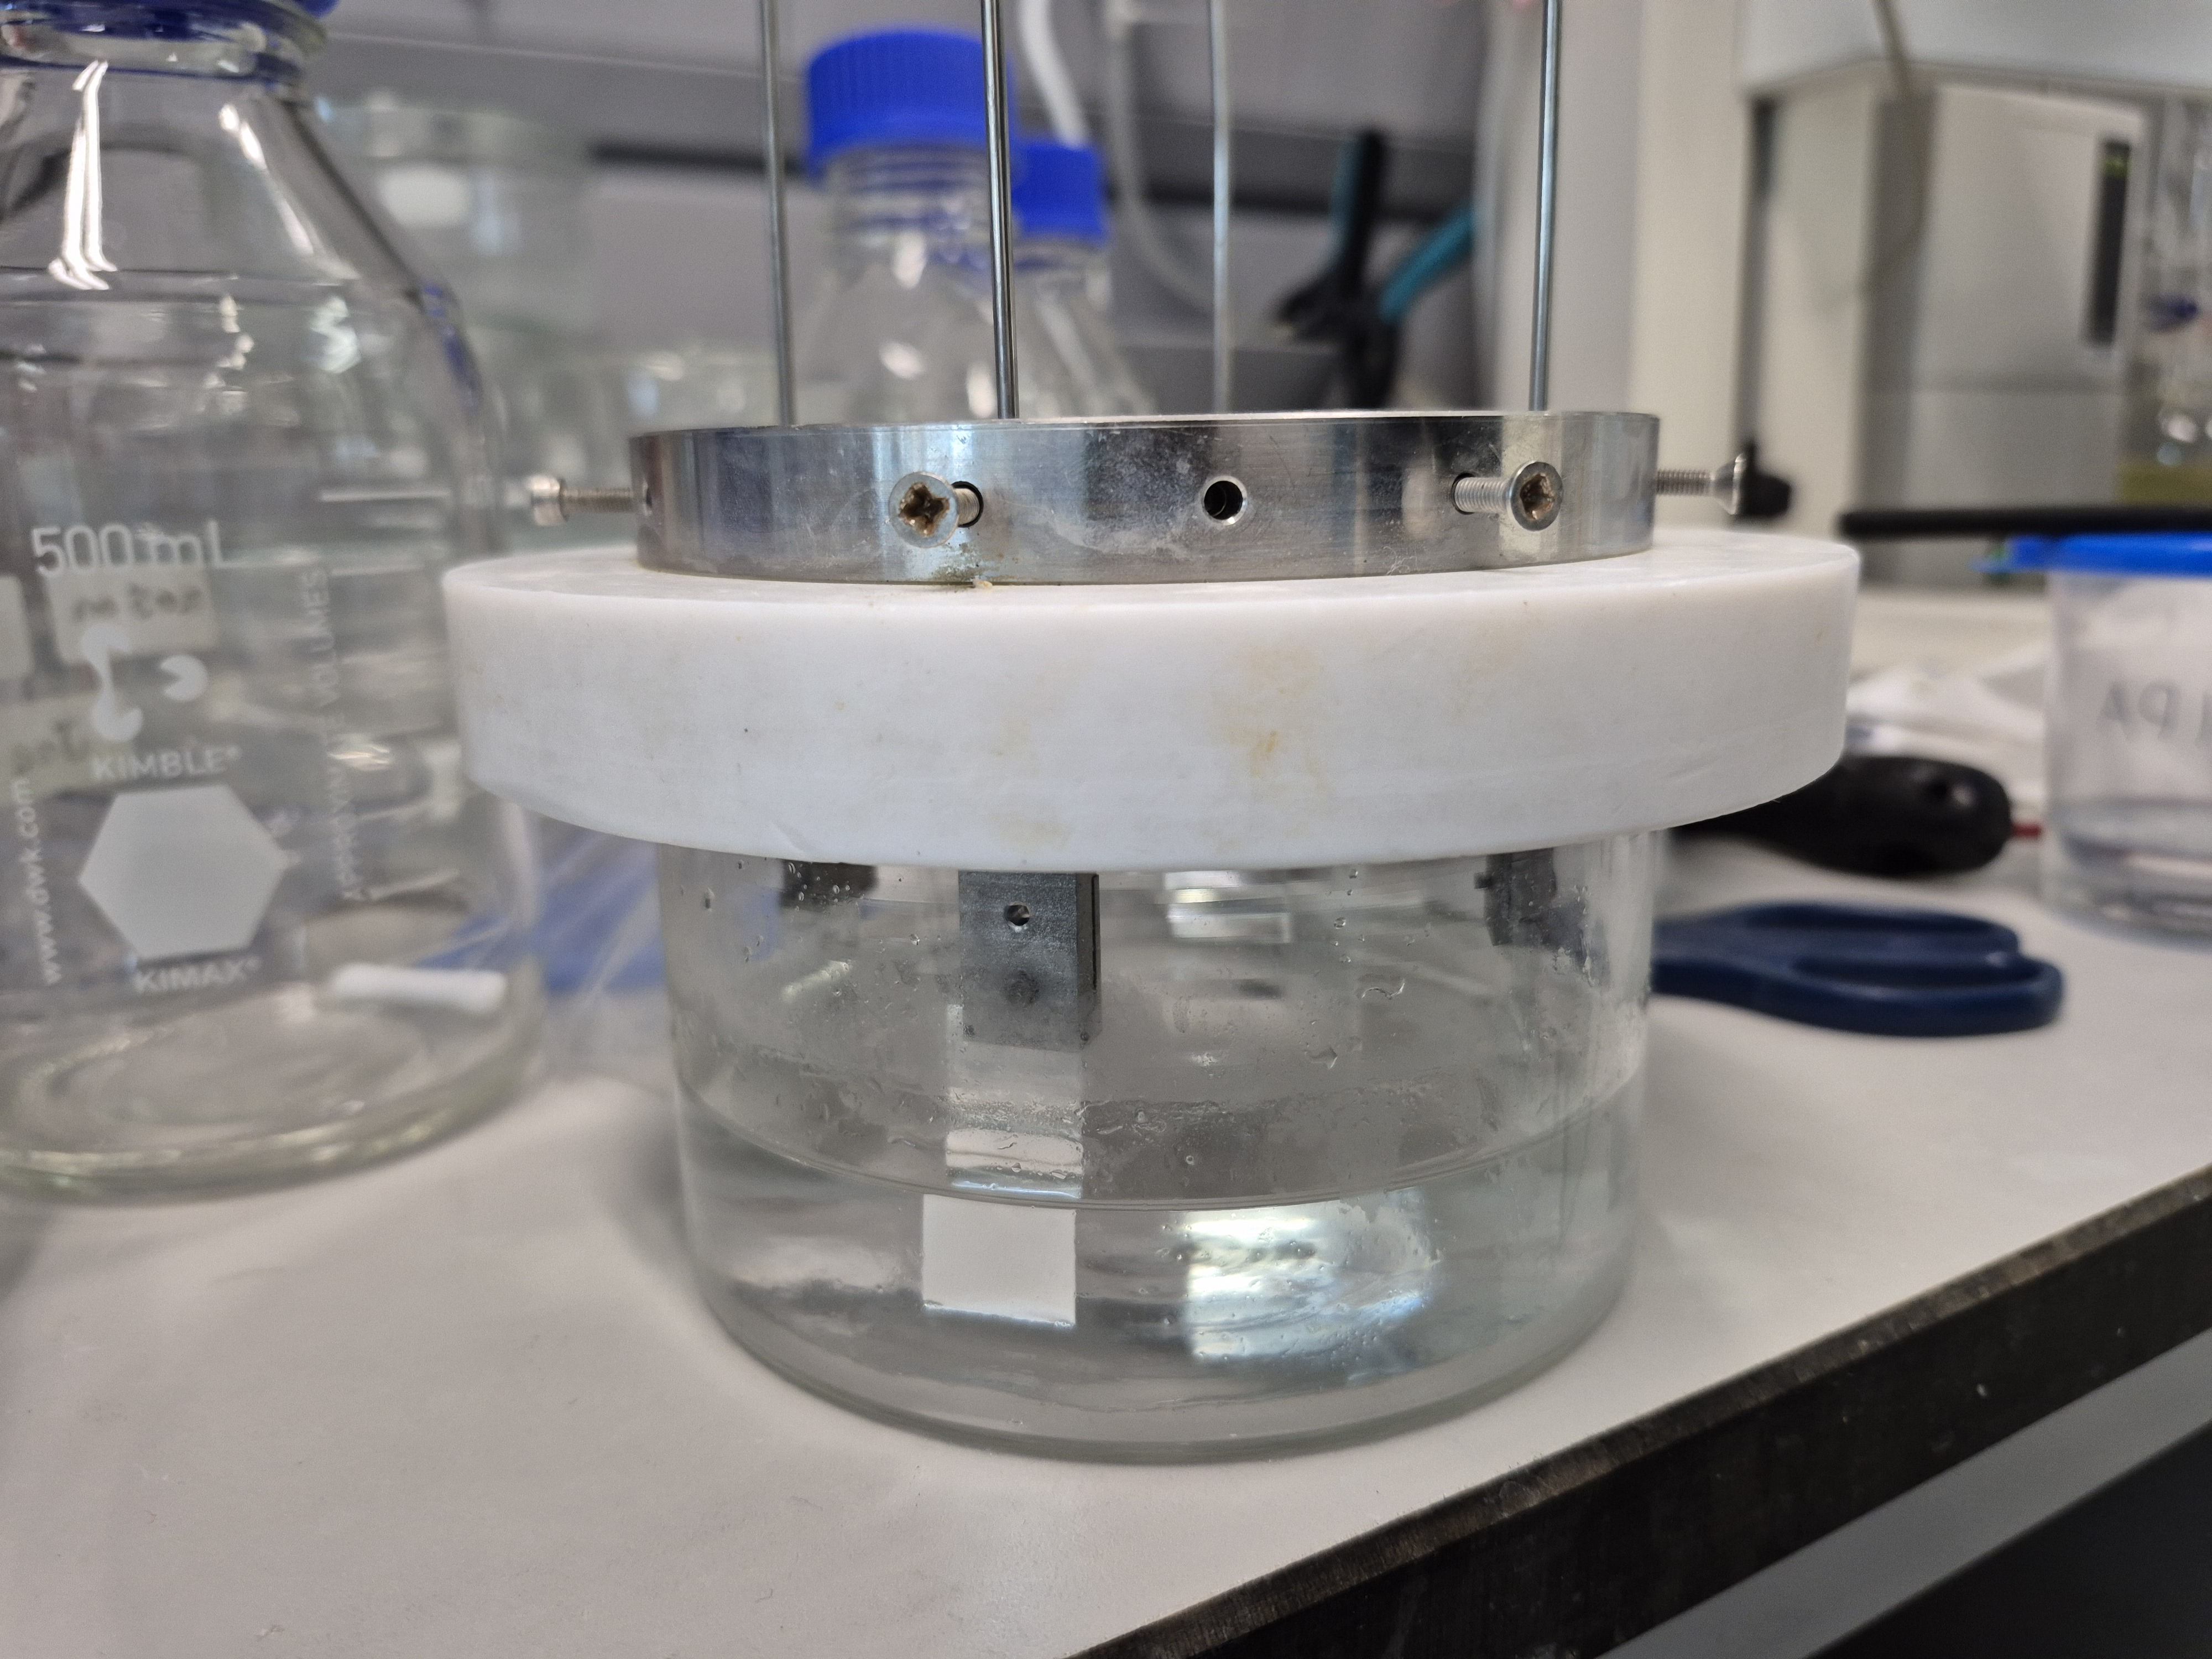
\includegraphics[width=\textwidth]{imgs/EC FA.jpg}
			\caption{First Anodization Electrochemical Cell}
			\label{fig:FAc}
		\end{subfigure}
		\hfill
		% Panel (b)
		\begin{subfigure}[b]{0.45\textwidth}
			\centering
			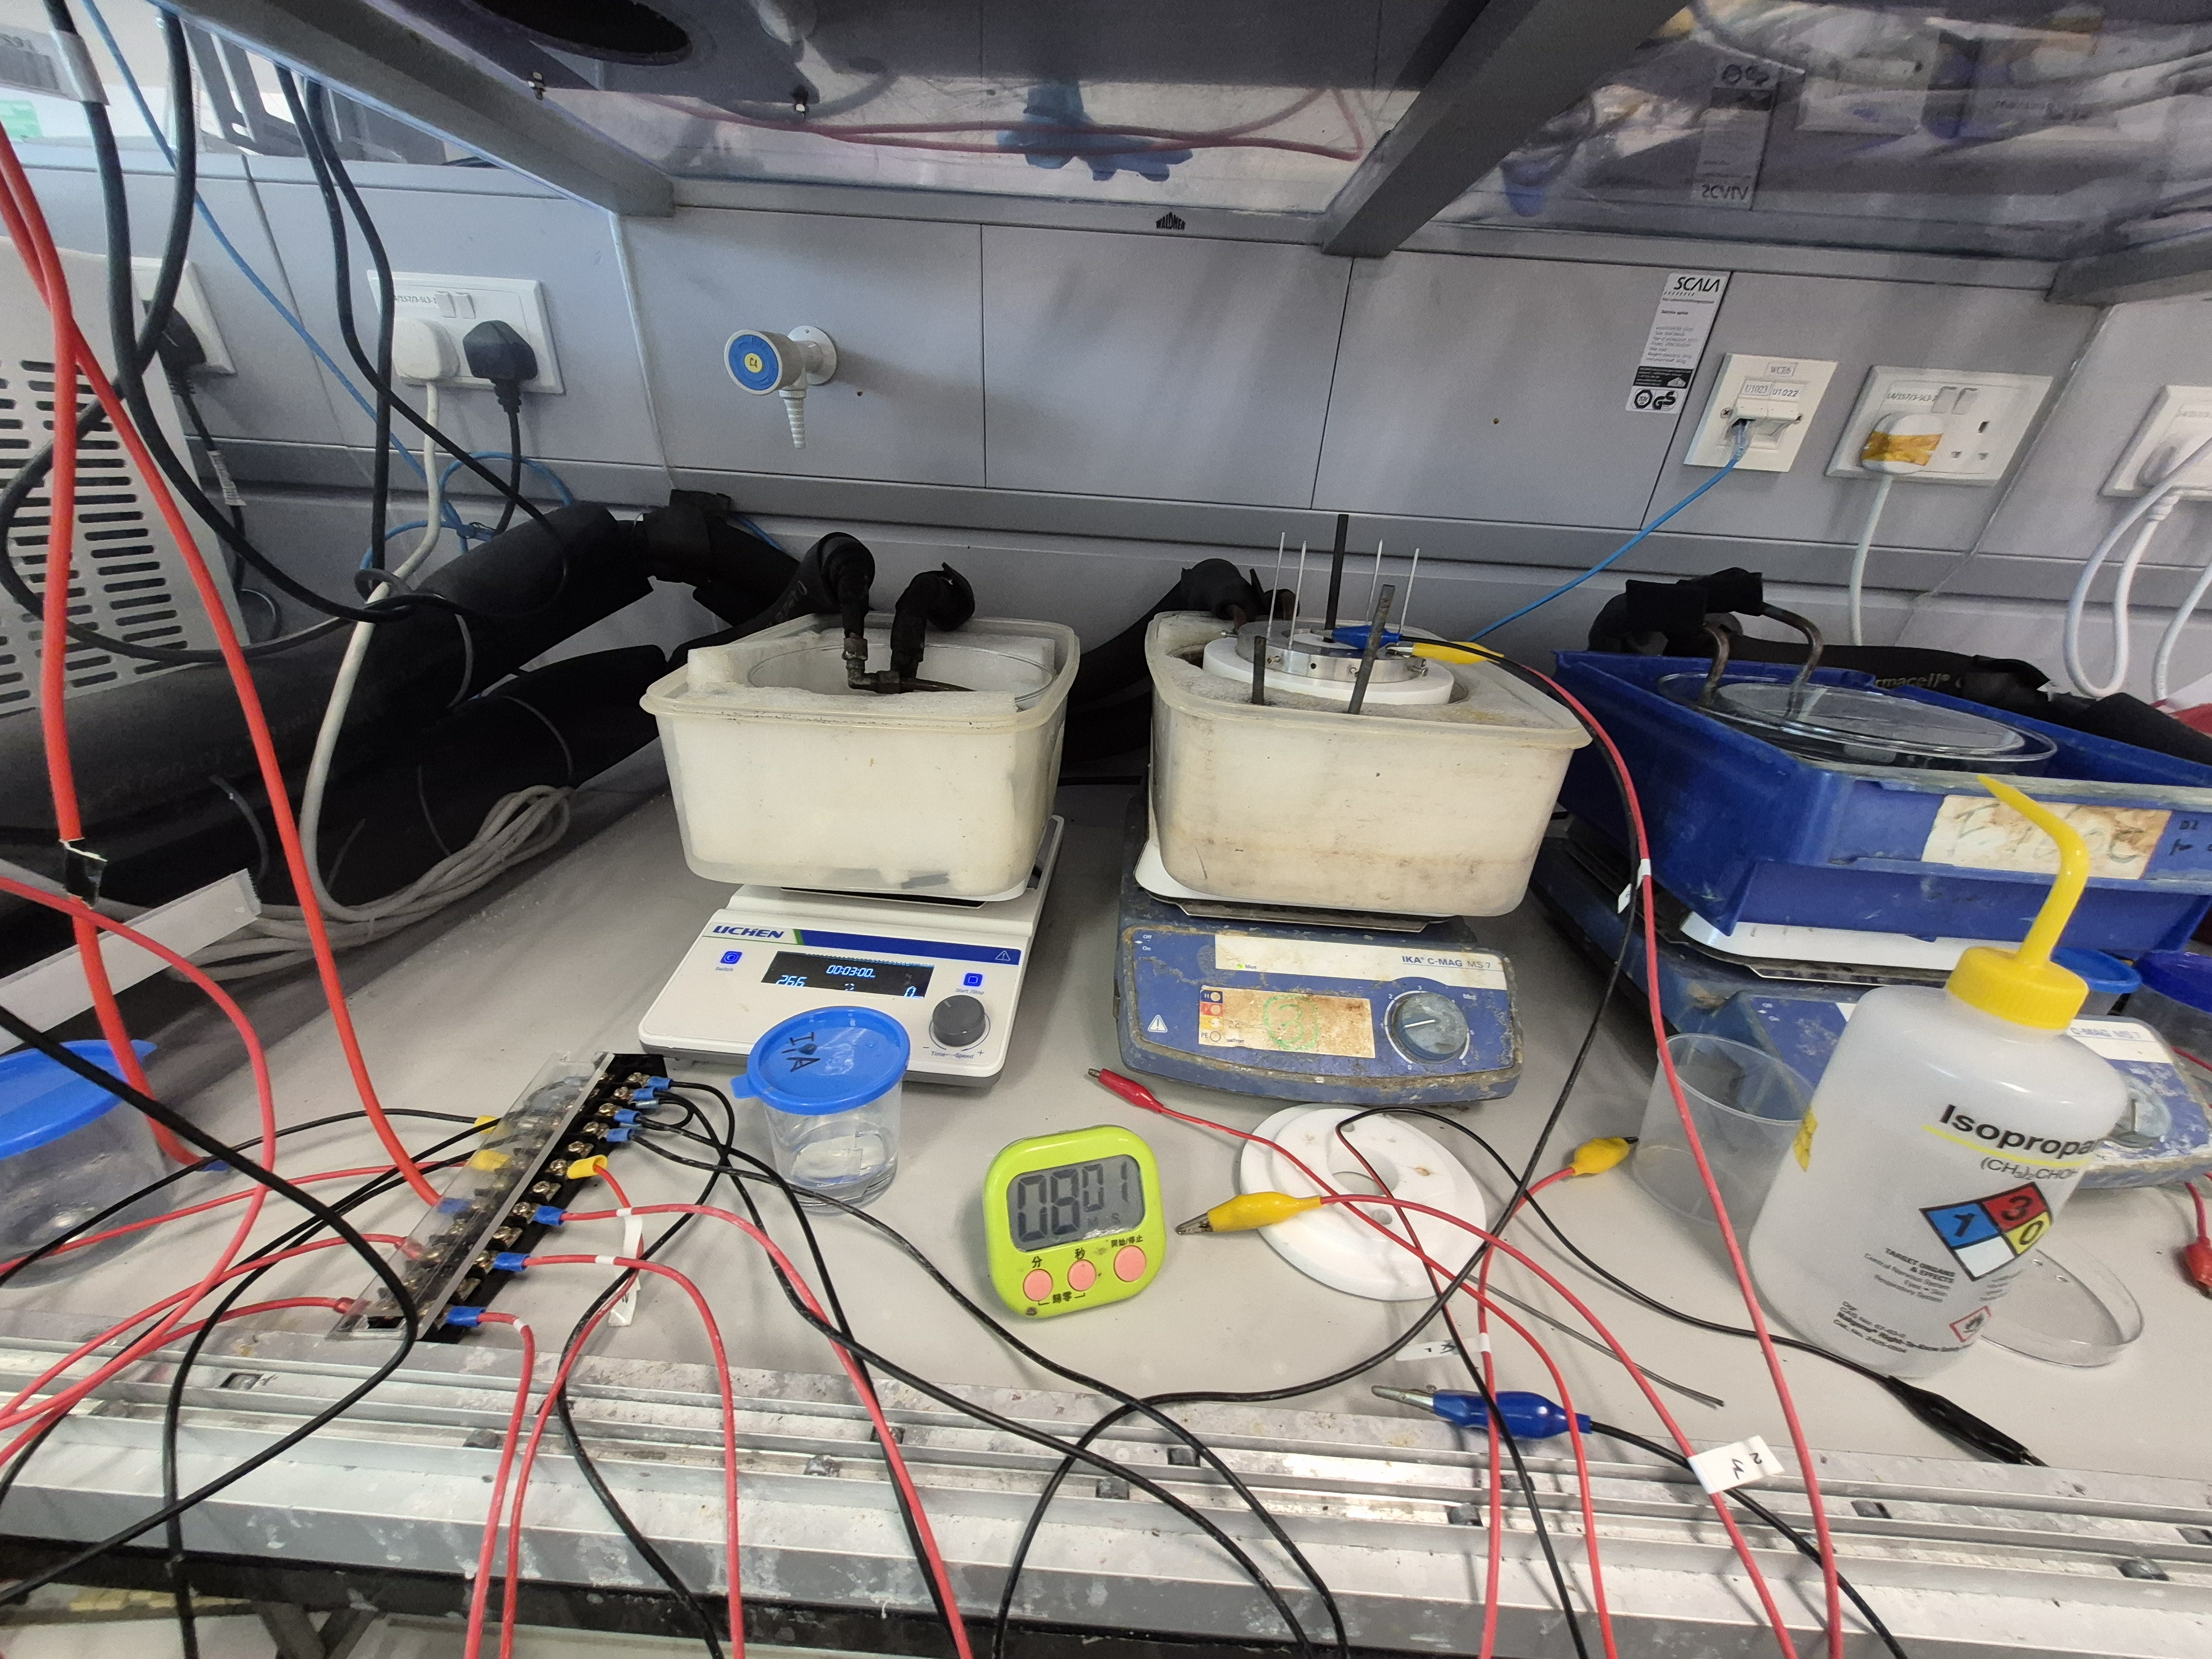
\includegraphics[width=\textwidth]{imgs/FA setup.jpg}
			\caption{First Anodization setup}
			\label{fig:FAS}
		\end{subfigure}
		
		\vspace{0.3cm} % optional spacing between rows
		
		% Panel (c)
		\begin{subfigure}[b]{0.45\textwidth}
			\centering
			\includegraphics[width=\textwidth,angle=-90]{imgs/FA res.jpg}
			\caption{Aluminum Chip after First Anodization}
			\label{fig:FAR}
		\end{subfigure}
		\hfill
		\begin{subfigure}[b]{0.45\textwidth}
			\centering
			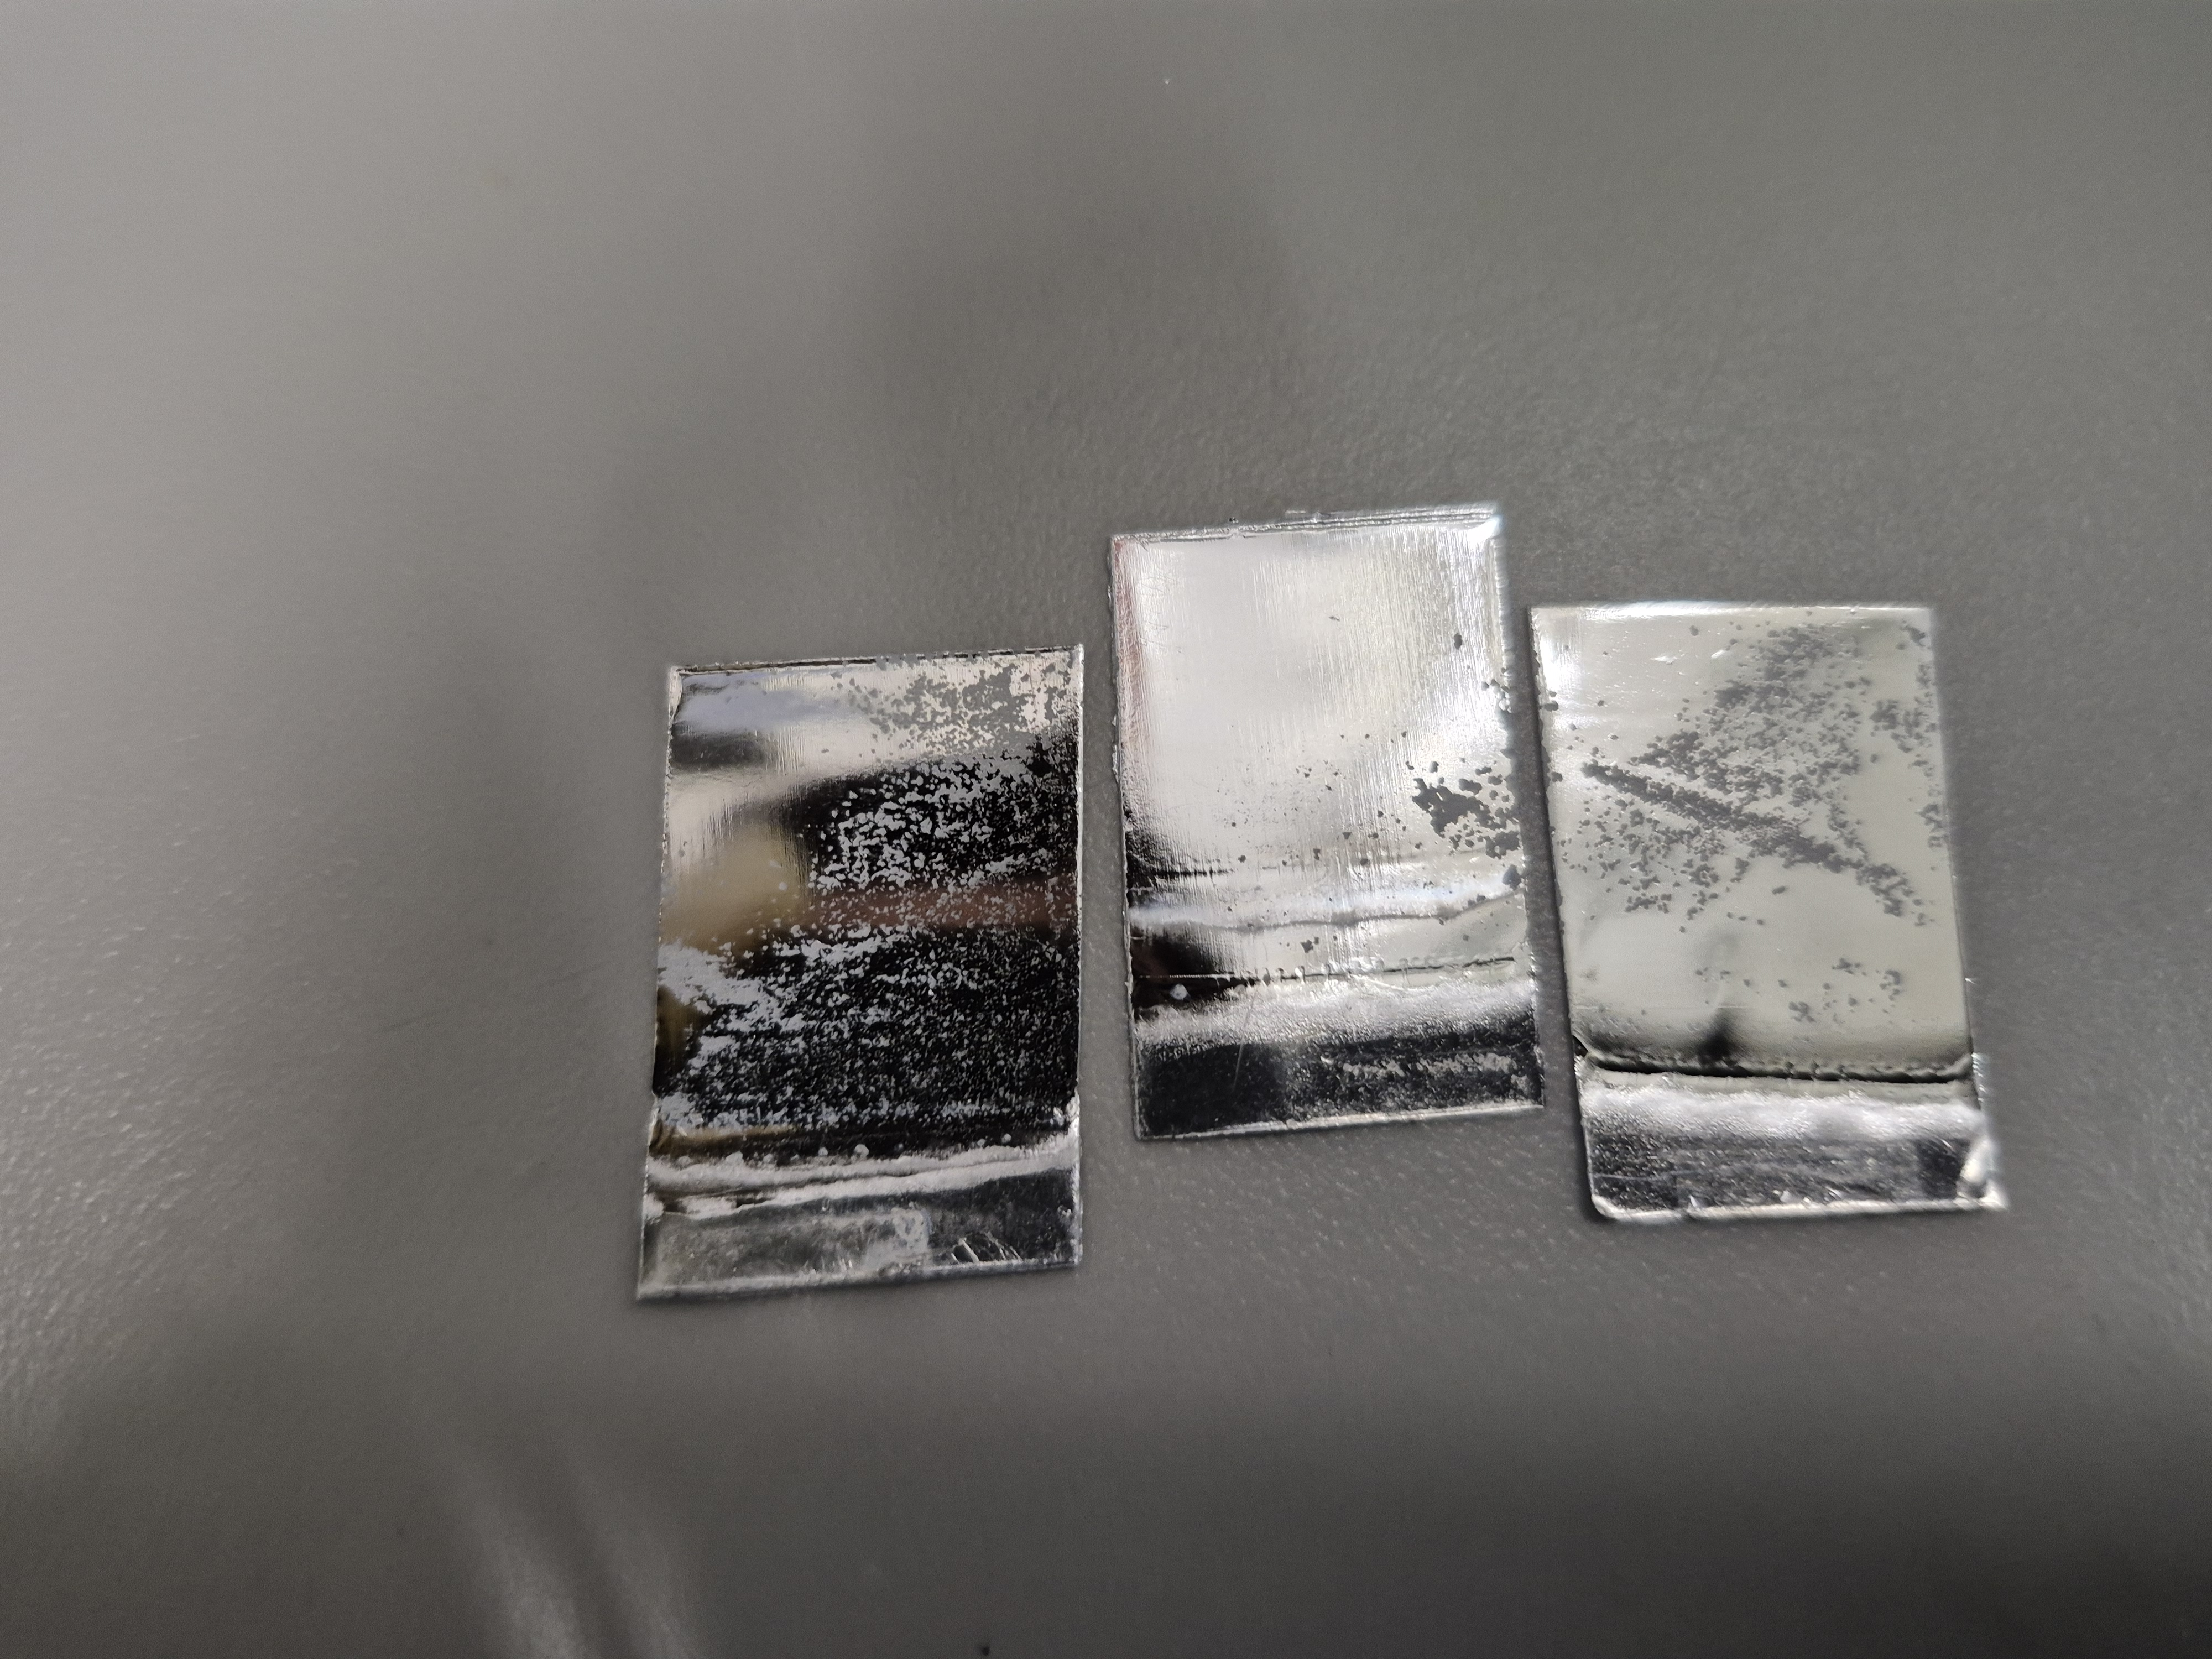
\includegraphics[width=\textwidth]{imgs/burnt.jpg}
			\caption{Burnt chips during the First Anodization}
			\label{fig:FAB}
		\end{subfigure}
		
		\caption{Step-by-step First Anodization process.}
		\label{fig:FA}
	\end{figure}
	
	\subsubsection{Etching Away the First Anodized Layer}
	
	After completing the first anodization, the resulting porous alumina layer was chemically removed to expose the pre-patterned aluminum surface beneath. This step is essential for achieving a more ordered pore arrangement during the subsequent anodization. The etching was carried out in a mixed acidic solution containing 6 wt\% phosphoric acid (\ce{H3PO4}) and 1.8 wt\% chromic acid (\ce{CrO3}), maintained at 98 °C for 30 minutes. The high temperature and strong oxidizing environment of this mixture effectively dissolve the initially formed oxide layer without damaging the underlying aluminum substrate (Figure \ref{fig:etch}) \cite{gu20163d}.
	
	During the etching process, the previously generated disordered pores serve as a template imprint on the aluminum surface, resulting in a periodic concave pattern once the oxide is fully removed. This pattern acts as a self-organized guide for the subsequent anodization step, leading to improved pore alignment and uniformity in the final AAO template. After etching, the samples were thoroughly rinsed with deionized water and gently dried under an air gun to remove any residual acid and prevent surface contamination before the second anodization \cite{gu20163d} .
	
	\begin{figure}[htpb]
		\centering
		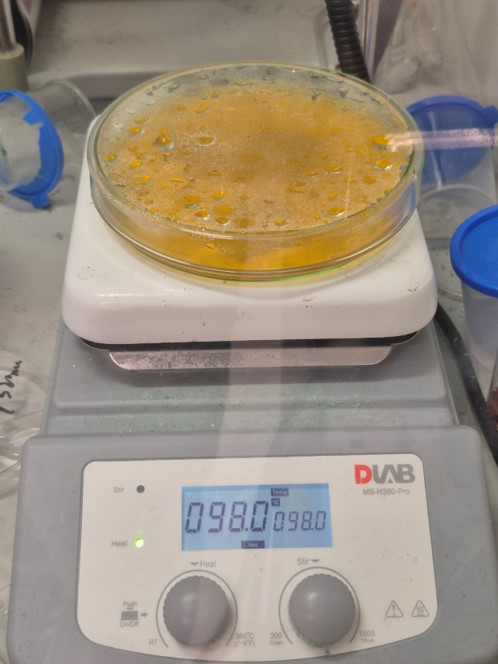
\includegraphics[width=0.5\textwidth]{imgs/etch.jpg}
		
		\caption{The Etching process setup}
		\label{fig:etch}
	\end{figure}
	
	
	\subsubsection{Second Anodization}
	
	The second anodization was performed under the same experimental conditions as the first anodization to ensure comparable oxide growth characteristics. Following the selective removal of the first anodic alumina layer, the aluminum substrate exhibited a highly ordered dimpled surface that acted as a template for pore nucleation.
	
	Using the same electrolyte, voltage, and temperature parameters as described in Section \ref{sec:FirstAnodization}, the second anodization was conducted for the same duration to obtain a porous anodic alumina (PAA) layer with improved pore ordering and uniformity. The pre-textured aluminum surface facilitated self-organization of the pores, leading to a more regular hexagonal arrangement compared to the first anodization.
	
	\subsubsection{Barrier Layer Thinning}
	
	To enable subsequent electrochemical deposition of Pb nanoclusters, the insulating barrier layer at the bottom of the porous anodic alumina (PAA) template was thinned by a controlled voltage ramping process. This step was carried out in $0.2$ M phosphoric acid (\ce{H3PO4}) solution at room temperature. The anodization system consisted of a Keithley 2400 source meter controlled by a computer program, which allowed precise adjustment of the applied voltage and current (Figure \ref{fig:BTcell}).
	
	At the beginning of the process, the system operated in voltage-source mode, where the anodization voltage was gradually increased to $160~V$, and the corresponding steady-state current $I_0$ was recorded. Subsequently, the instrument was switched to current-source mode and the current was fixed at $\frac{I_0}{2}$. A gradual reduction in voltage was observed as the barrier layer began to dissolve and thin under field-assisted conditions. Once the rate of voltage decline slowed to approximately $3~V min^{-1}$, the measured voltage had typically decreased to about $80~V$. The current was then further reduced to $\frac{I_0}{4}$ to accelerate the final stage of barrier thinning. When the voltage reached $4~V$, the process was terminated (Figure \ref{fig:BTp}).
	
	This controlled voltage ramping enabled uniform reduction of the barrier layer thickness down to a few nanometers (approximately $4~nm$), which is sufficient to allow quantum tunneling of electrons between the aluminum substrate and the pore bases. The total duration of the barrier thinning process was approximately $20$ minutes.
	
	\begin{figure}[htpb]
		\centering
		% Panel (a)
		\begin{subfigure}[b]{0.45\textwidth}
			\centering
			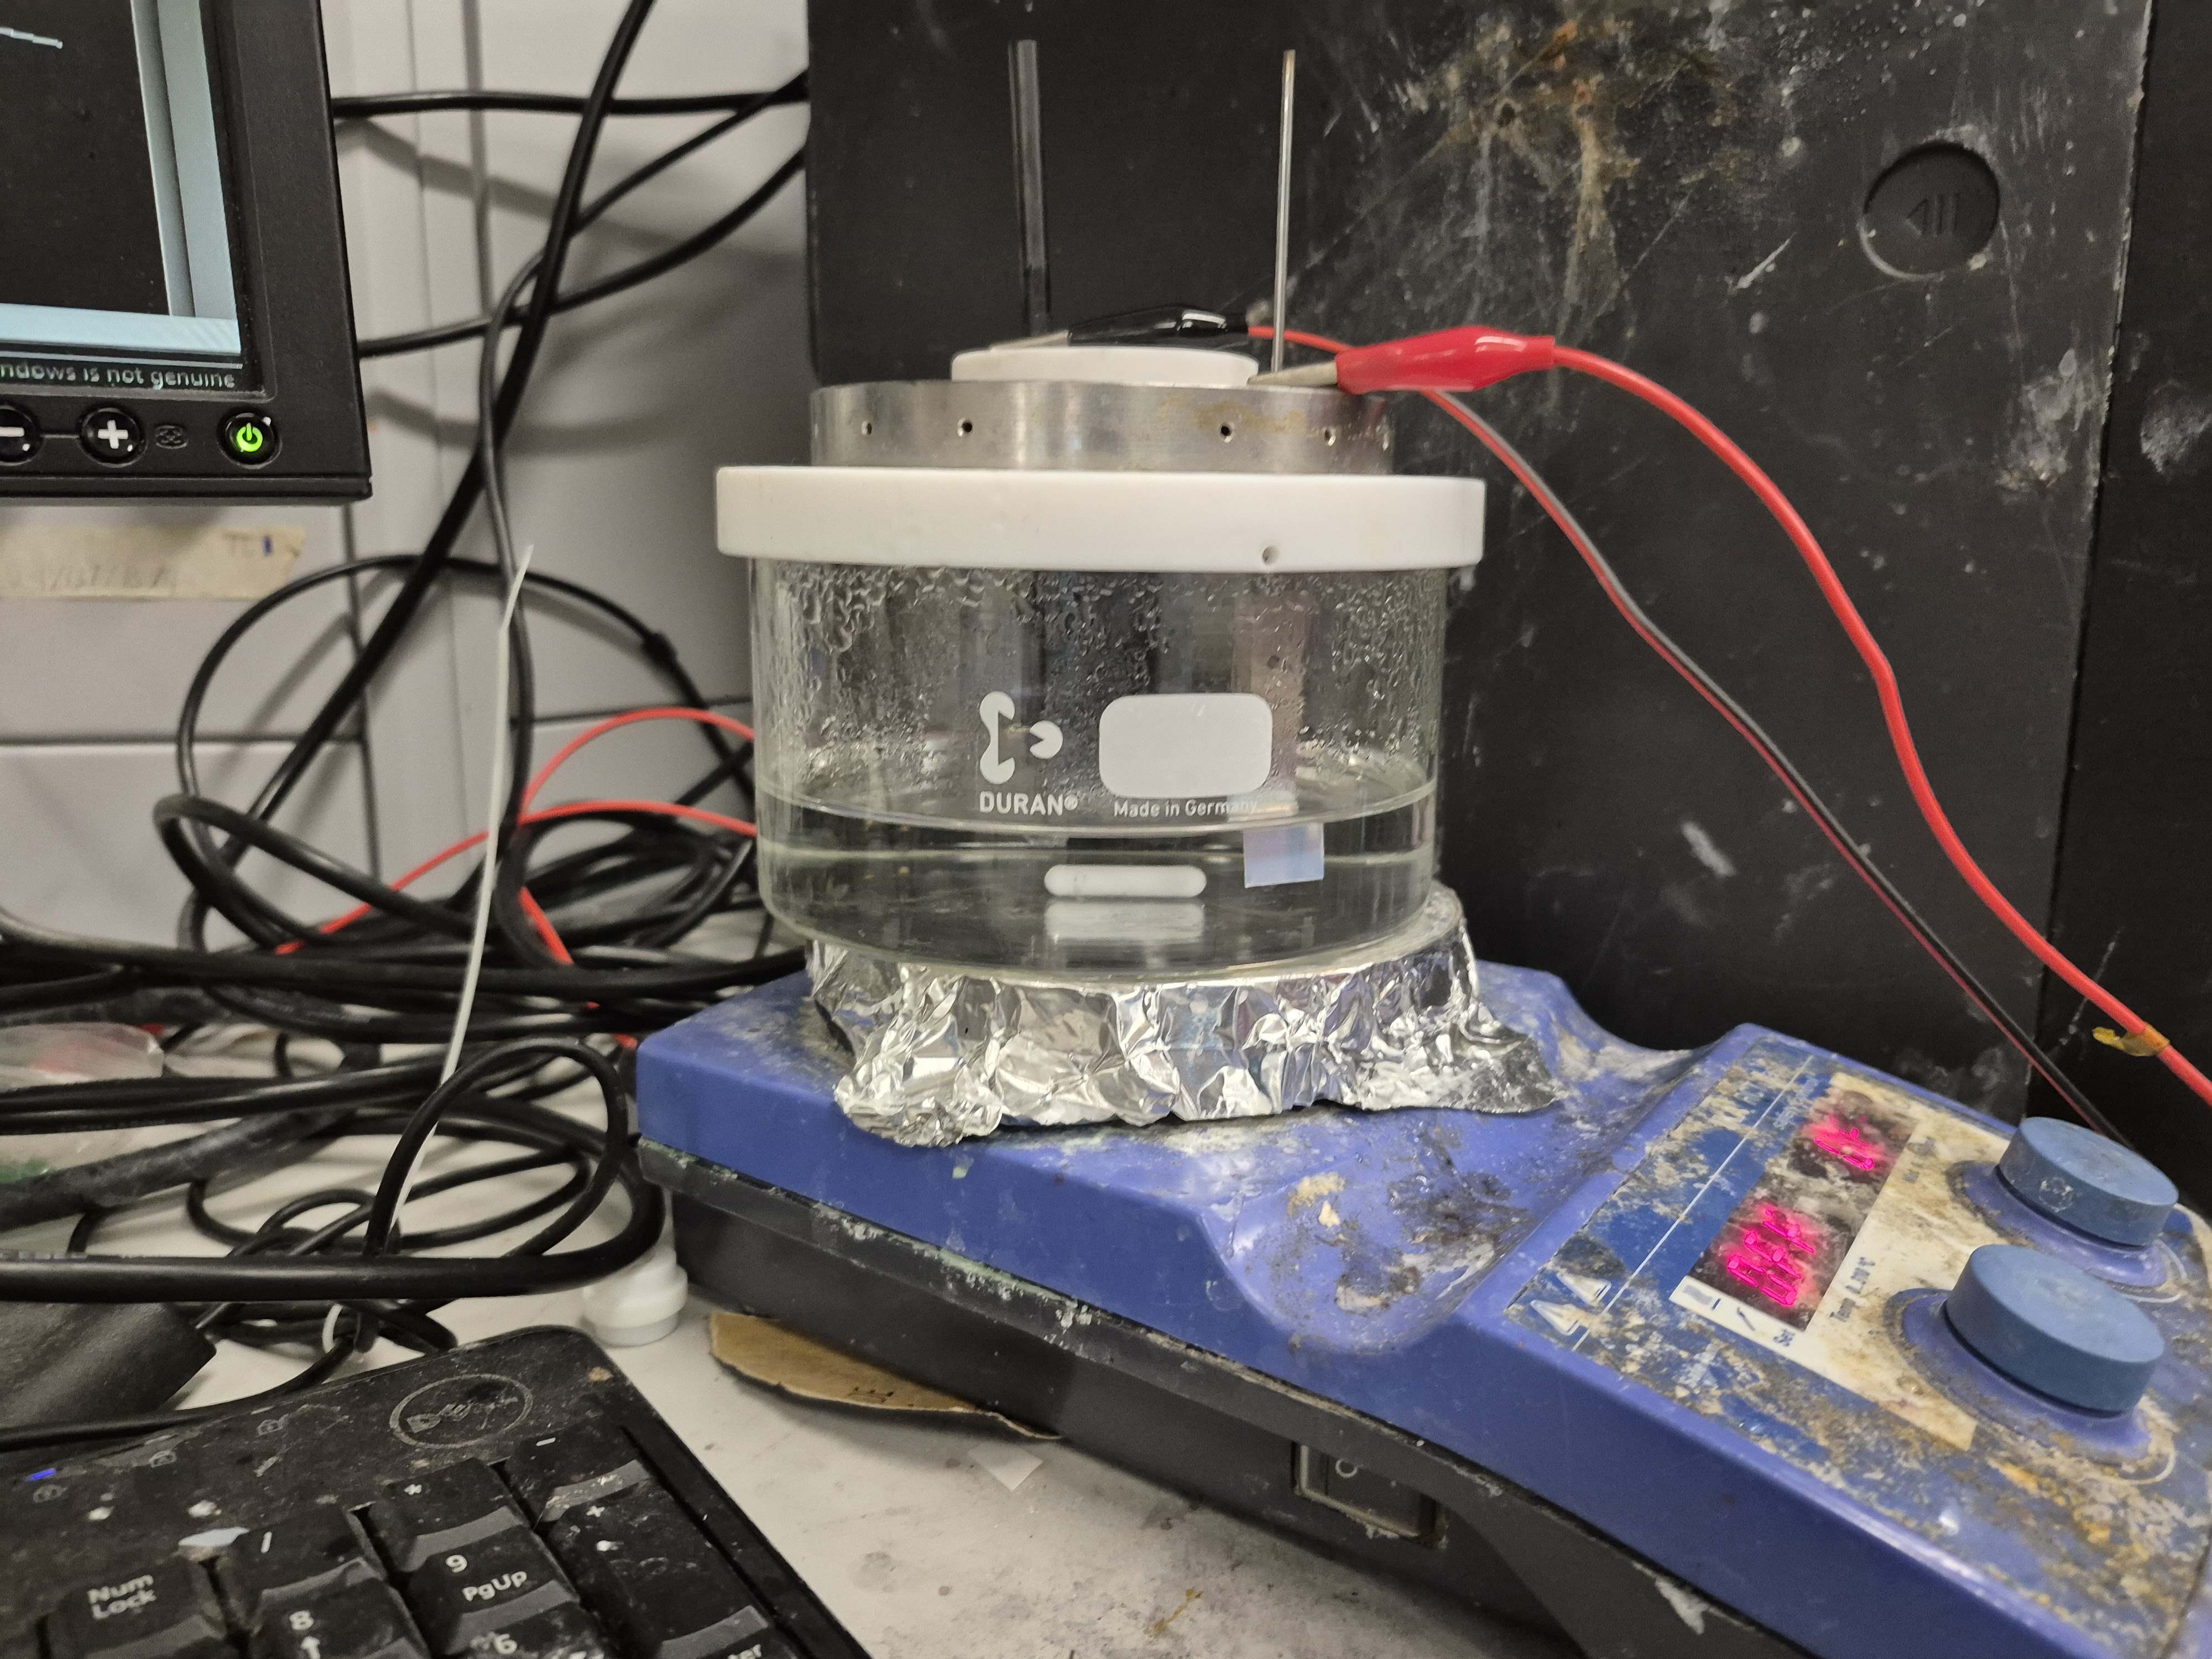
\includegraphics[width=\textwidth]{imgs/BTcell.jpg}
			\caption{Barrier Thinning Electrochemical Cell setup}
			\label{fig:BTcell}
		\end{subfigure}
		\hfill
		% Panel (b)
		\begin{subfigure}[b]{0.45\textwidth}
			\centering
			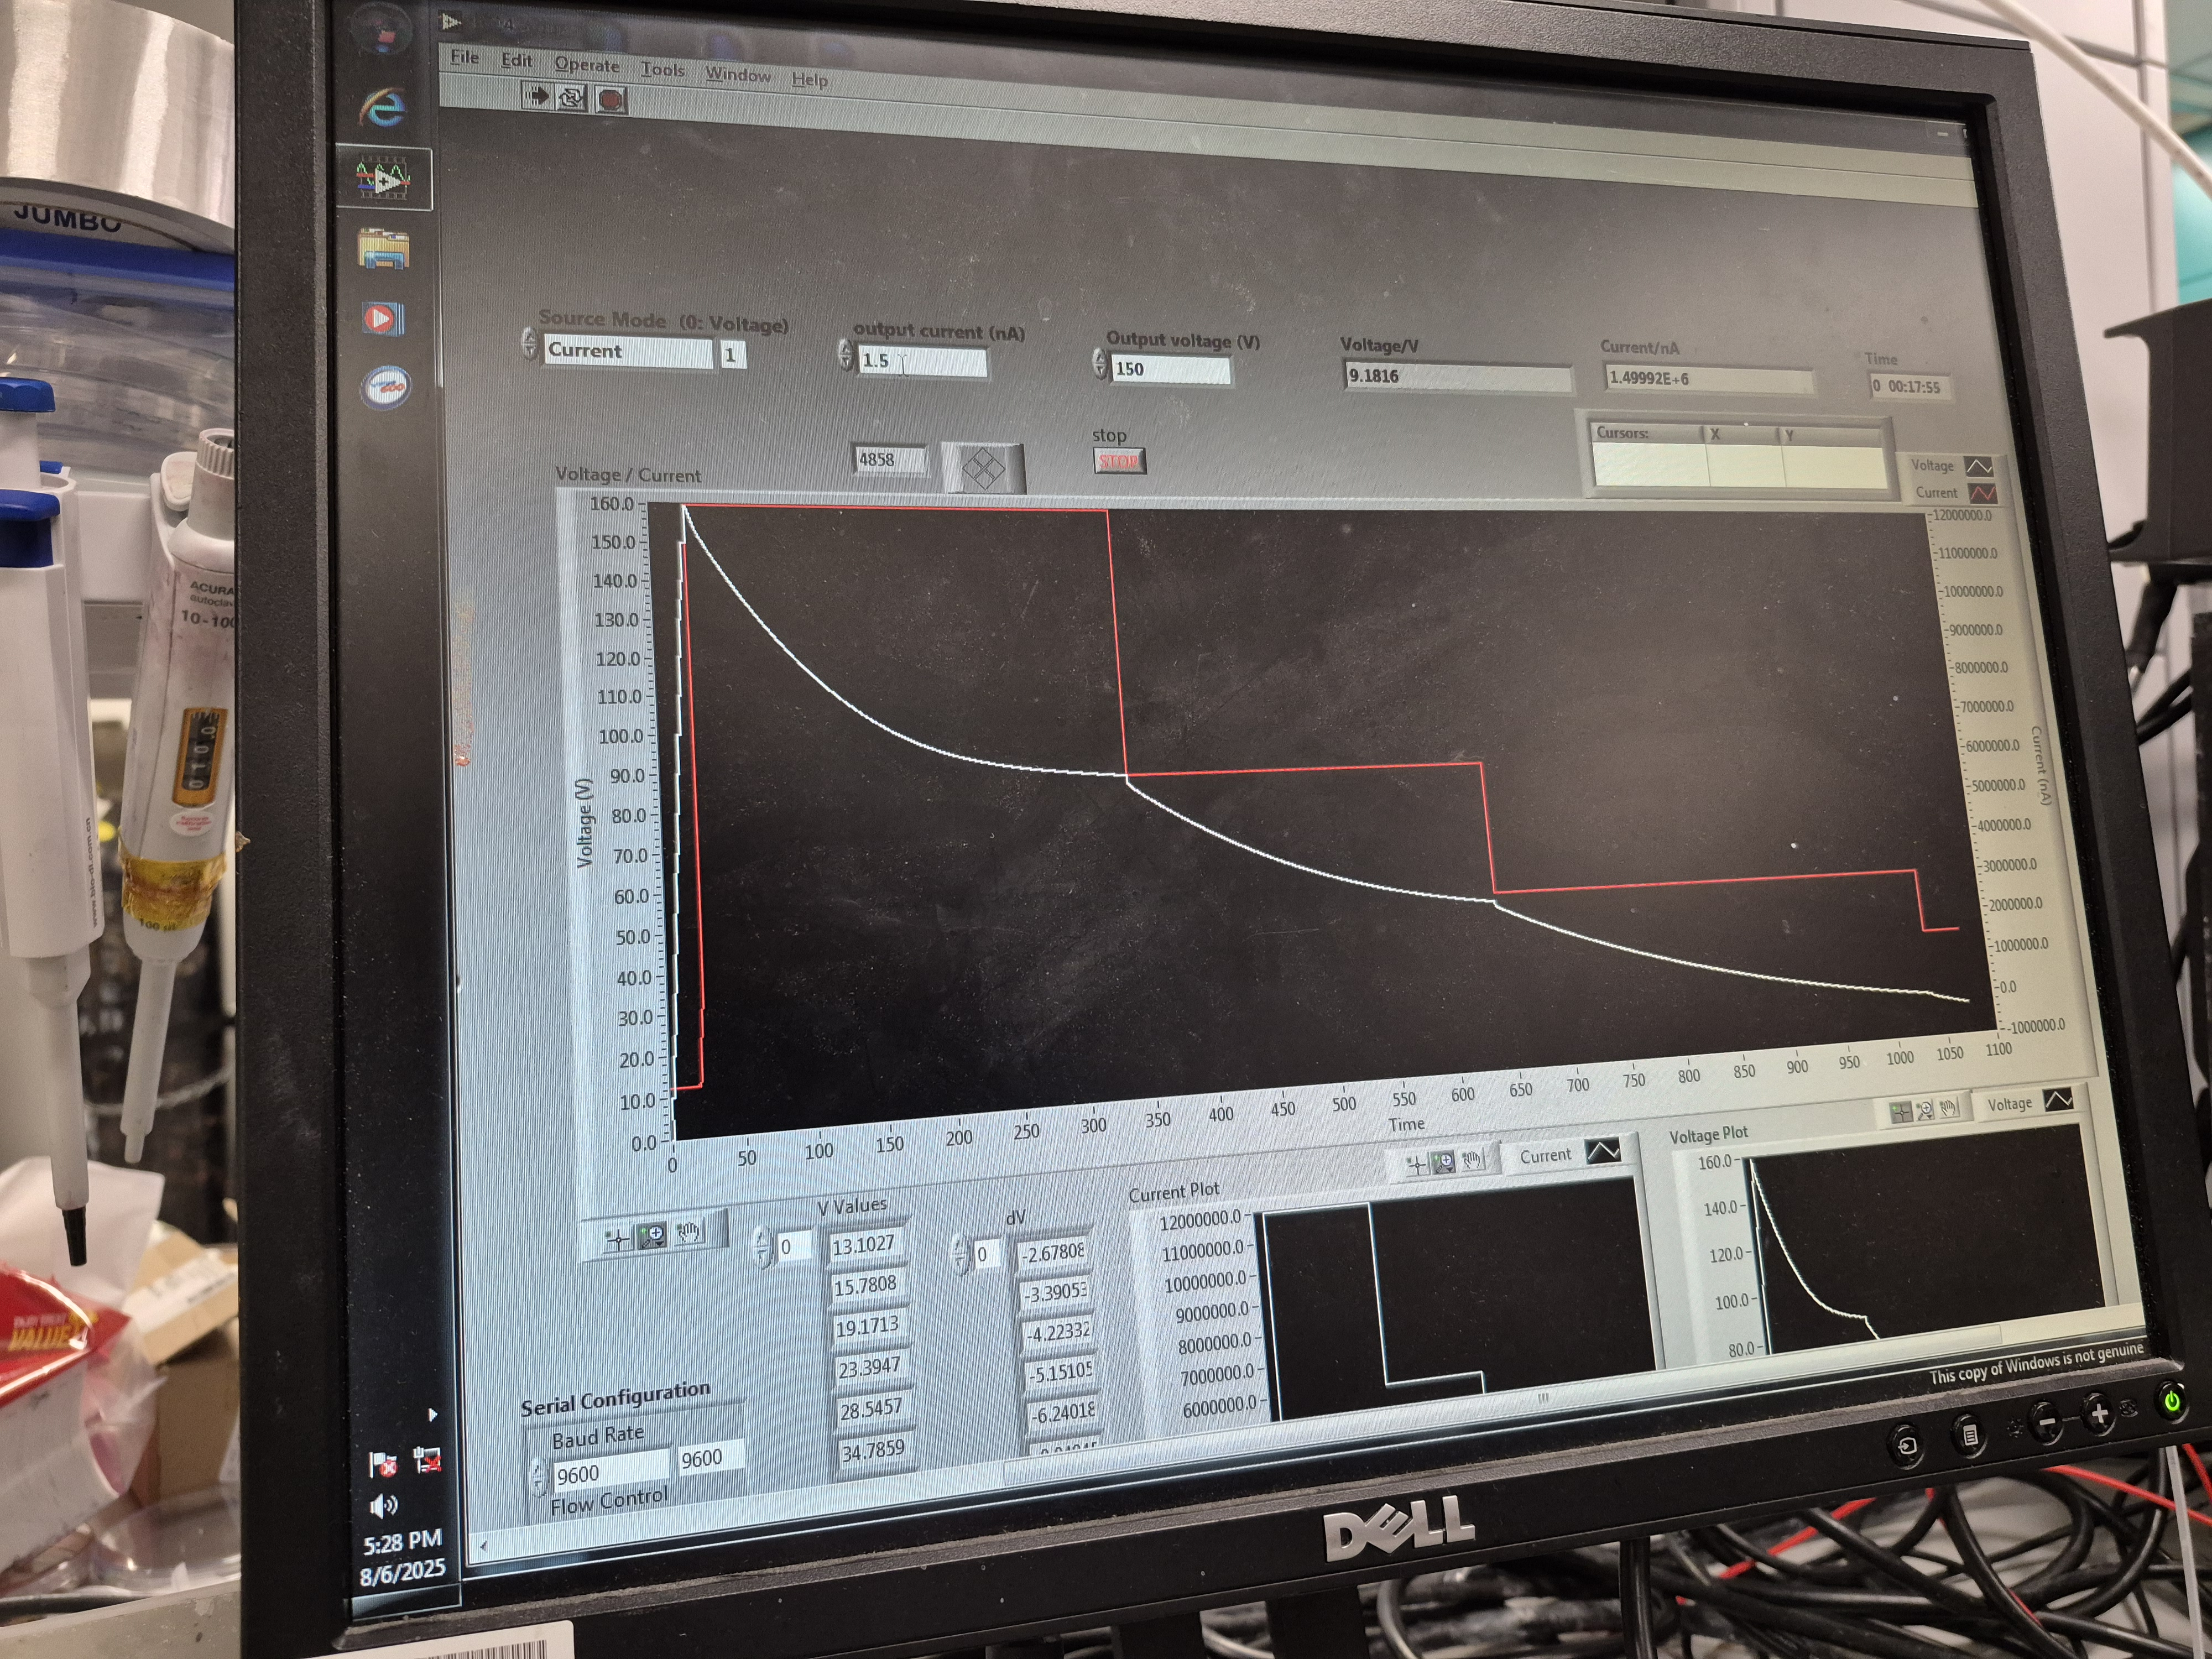
\includegraphics[width=\textwidth]{imgs/BTp.jpg}
			\caption{Barrier Thinning Process}
			\label{fig:BTp}
		\end{subfigure}
		
		\caption{Barrier Thinning Setup}
		\label{fig:BT}
	\end{figure}
	
	\subsubsection{Pb Electrodeposition}
	
	After the barrier layer thinning process, lead (\ce{Pb}) nanoclusters were electrochemically deposited at the bottom of the porous anodic alumina (PAA) channels using an alternating-current (AC) electrodeposition method. The deposition was performed in a three-electrode configuration controlled by a potentiostat (SG 300, Gamry Instruments). The PAA sample, with its underlying aluminum substrate, served as the working electrode, a carbon rod was used as the counter electrode, and an \ce{Ag/AgCl} electrode was employed as the reference .
	
	The electrolyte solution was prepared by dissolving $1.7$ g of lead(II) chloride (\ce{PbCl2}) and $25$ g of trisodium citrate (\ce{Na3C6H5O7}) in $100$ mL of deionized water under vigorous stirring until complete dissolution. The citrate ions acted as complexing agents, stabilizing \ce{Pb^{2+}} in solution and preventing uncontrolled precipitation (Figure \ref{fig:EDcell}).
	
	During deposition, a sinusoidal voltage with a frequency of $50$ Hz was applied for $10$ minutes. The voltage amplitude was adjusted between $3.4$ V and $9$ V to maintain a peak current density of approximately $2.2 mA·cm^{-2}$ during the negative half-cycle, which corresponds to the reduction phase of \ce{Pb^{2+}} to metallic \ce{Pb}. The alternating nature of the current minimized charge accumulation and facilitated uniform deposition at the pore bases (Figure \ref{fig:EDsettings} and \ref{fig:EDp}).
	
	Upon completion of the process, the sample was thoroughly rinsed several times with deionized water to remove any residual electrolyte and adsorbed species. The resulting lead layer was approximately $200$ nm thick, forming a continuous metallic contact at the bottom of the pores (Figure \ref{fig:EDr}).
	
	\begin{figure}[htpb]
		\centering
		% Panel (a)
		\begin{subfigure}[b]{0.45\textwidth}
			\centering
			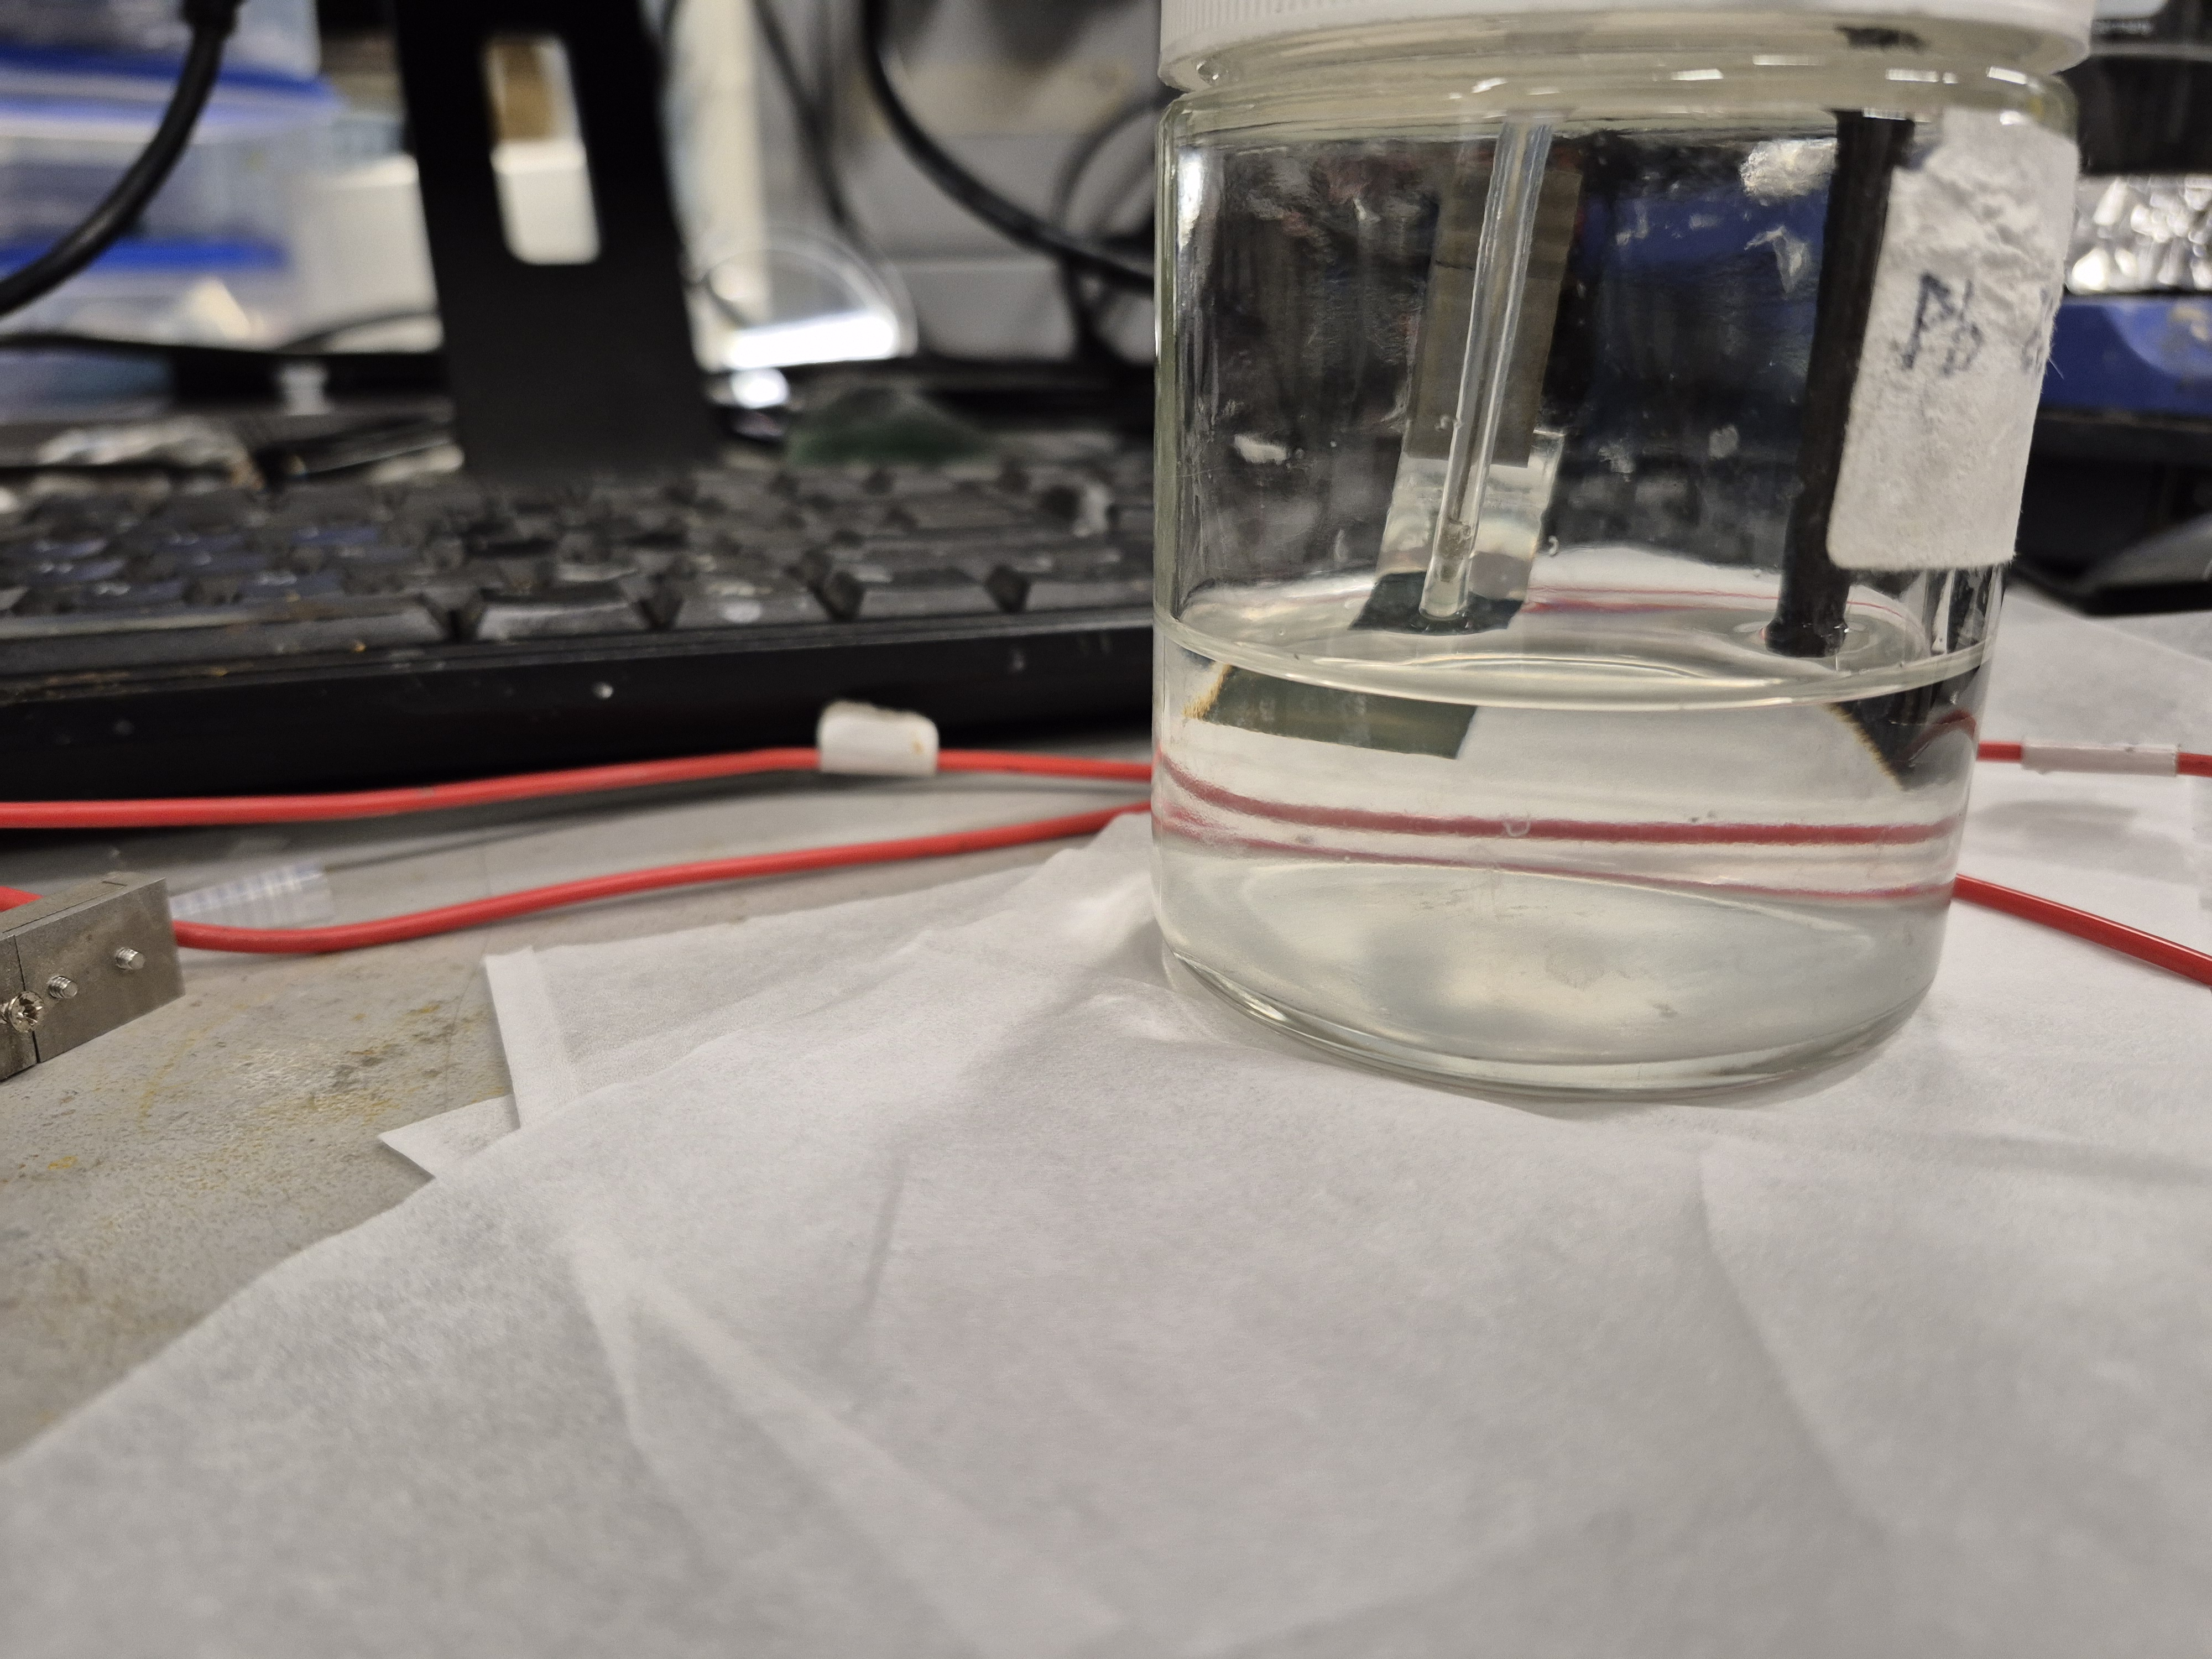
\includegraphics[width=\textwidth]{imgs/EDcell.jpg}
			\caption{Pb Electodeposition Electrochemical Cell}
			\label{fig:EDcell}
		\end{subfigure}
		\hfill
		% Panel (b)
		\begin{subfigure}[b]{0.45\textwidth}
			\centering
			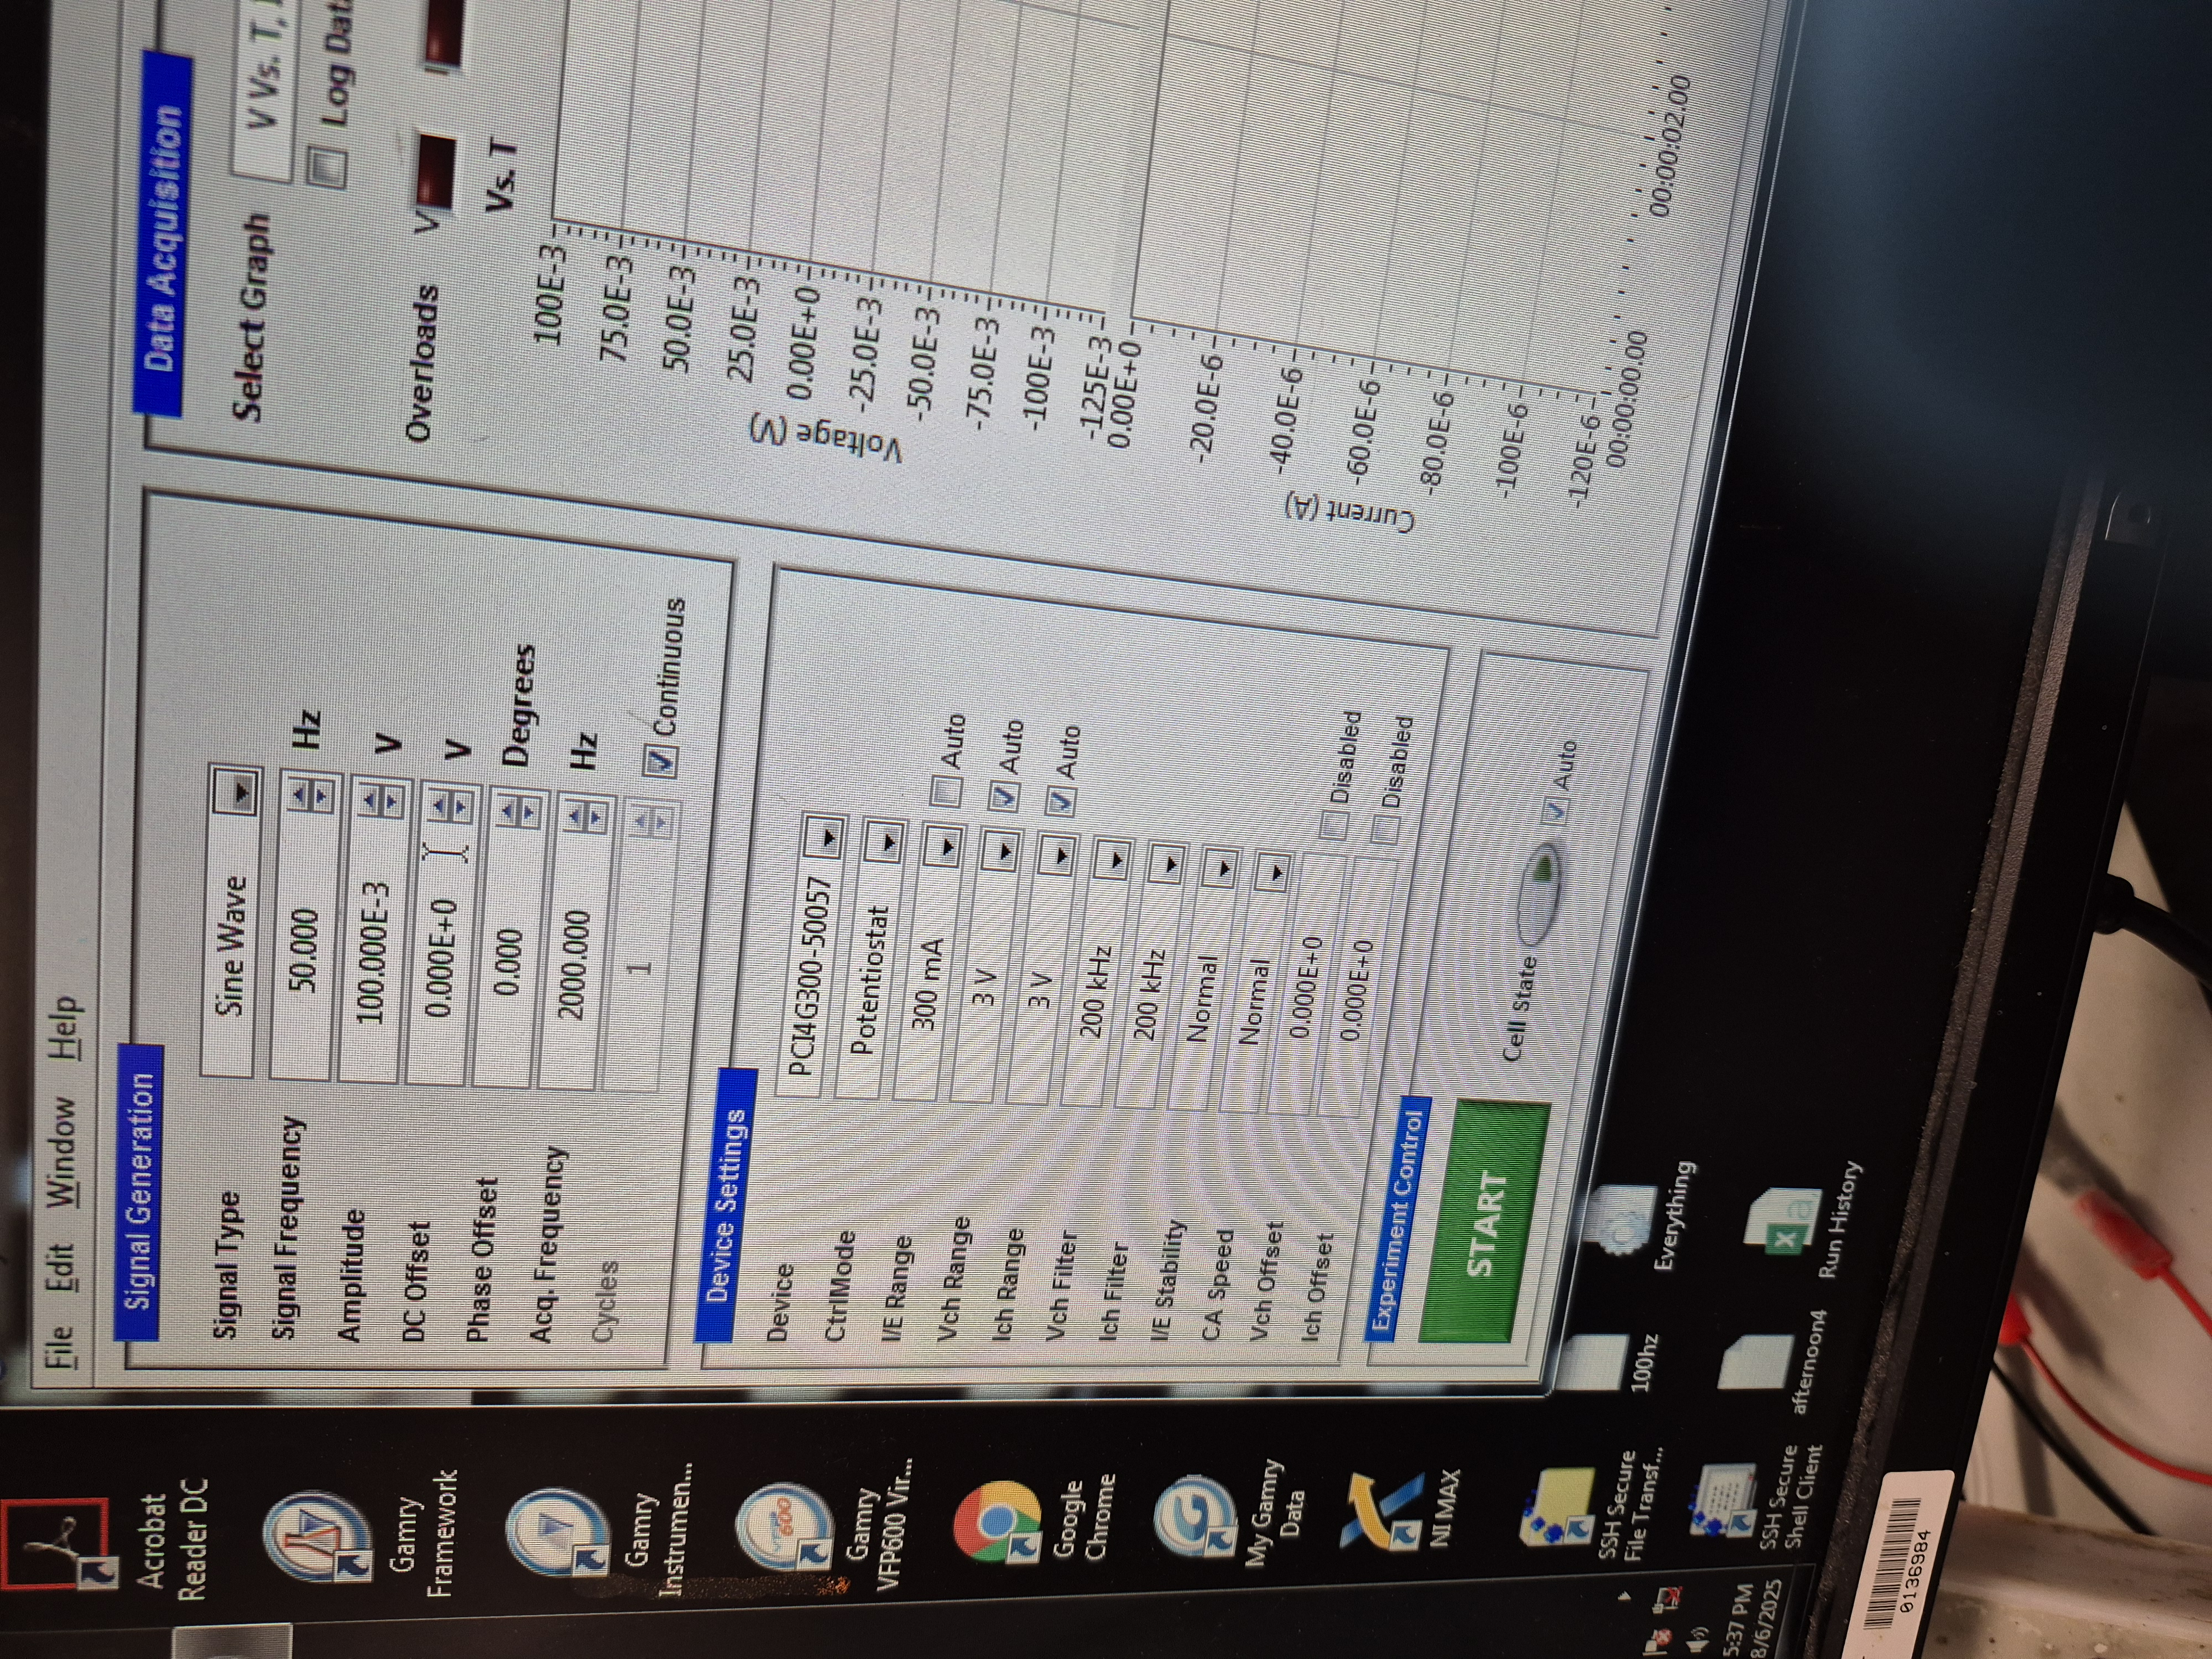
\includegraphics[width=\textwidth,angle=-90]{imgs/EDsettings.jpg}
			\caption{Pb Electrodeposition Parameter Tuning}
			\label{fig:EDsettings}
		\end{subfigure}
		
		\vspace{0.3cm} % optional spacing between rows
		
		% Panel (c)
		\begin{subfigure}[b]{0.45\textwidth}
			\centering
			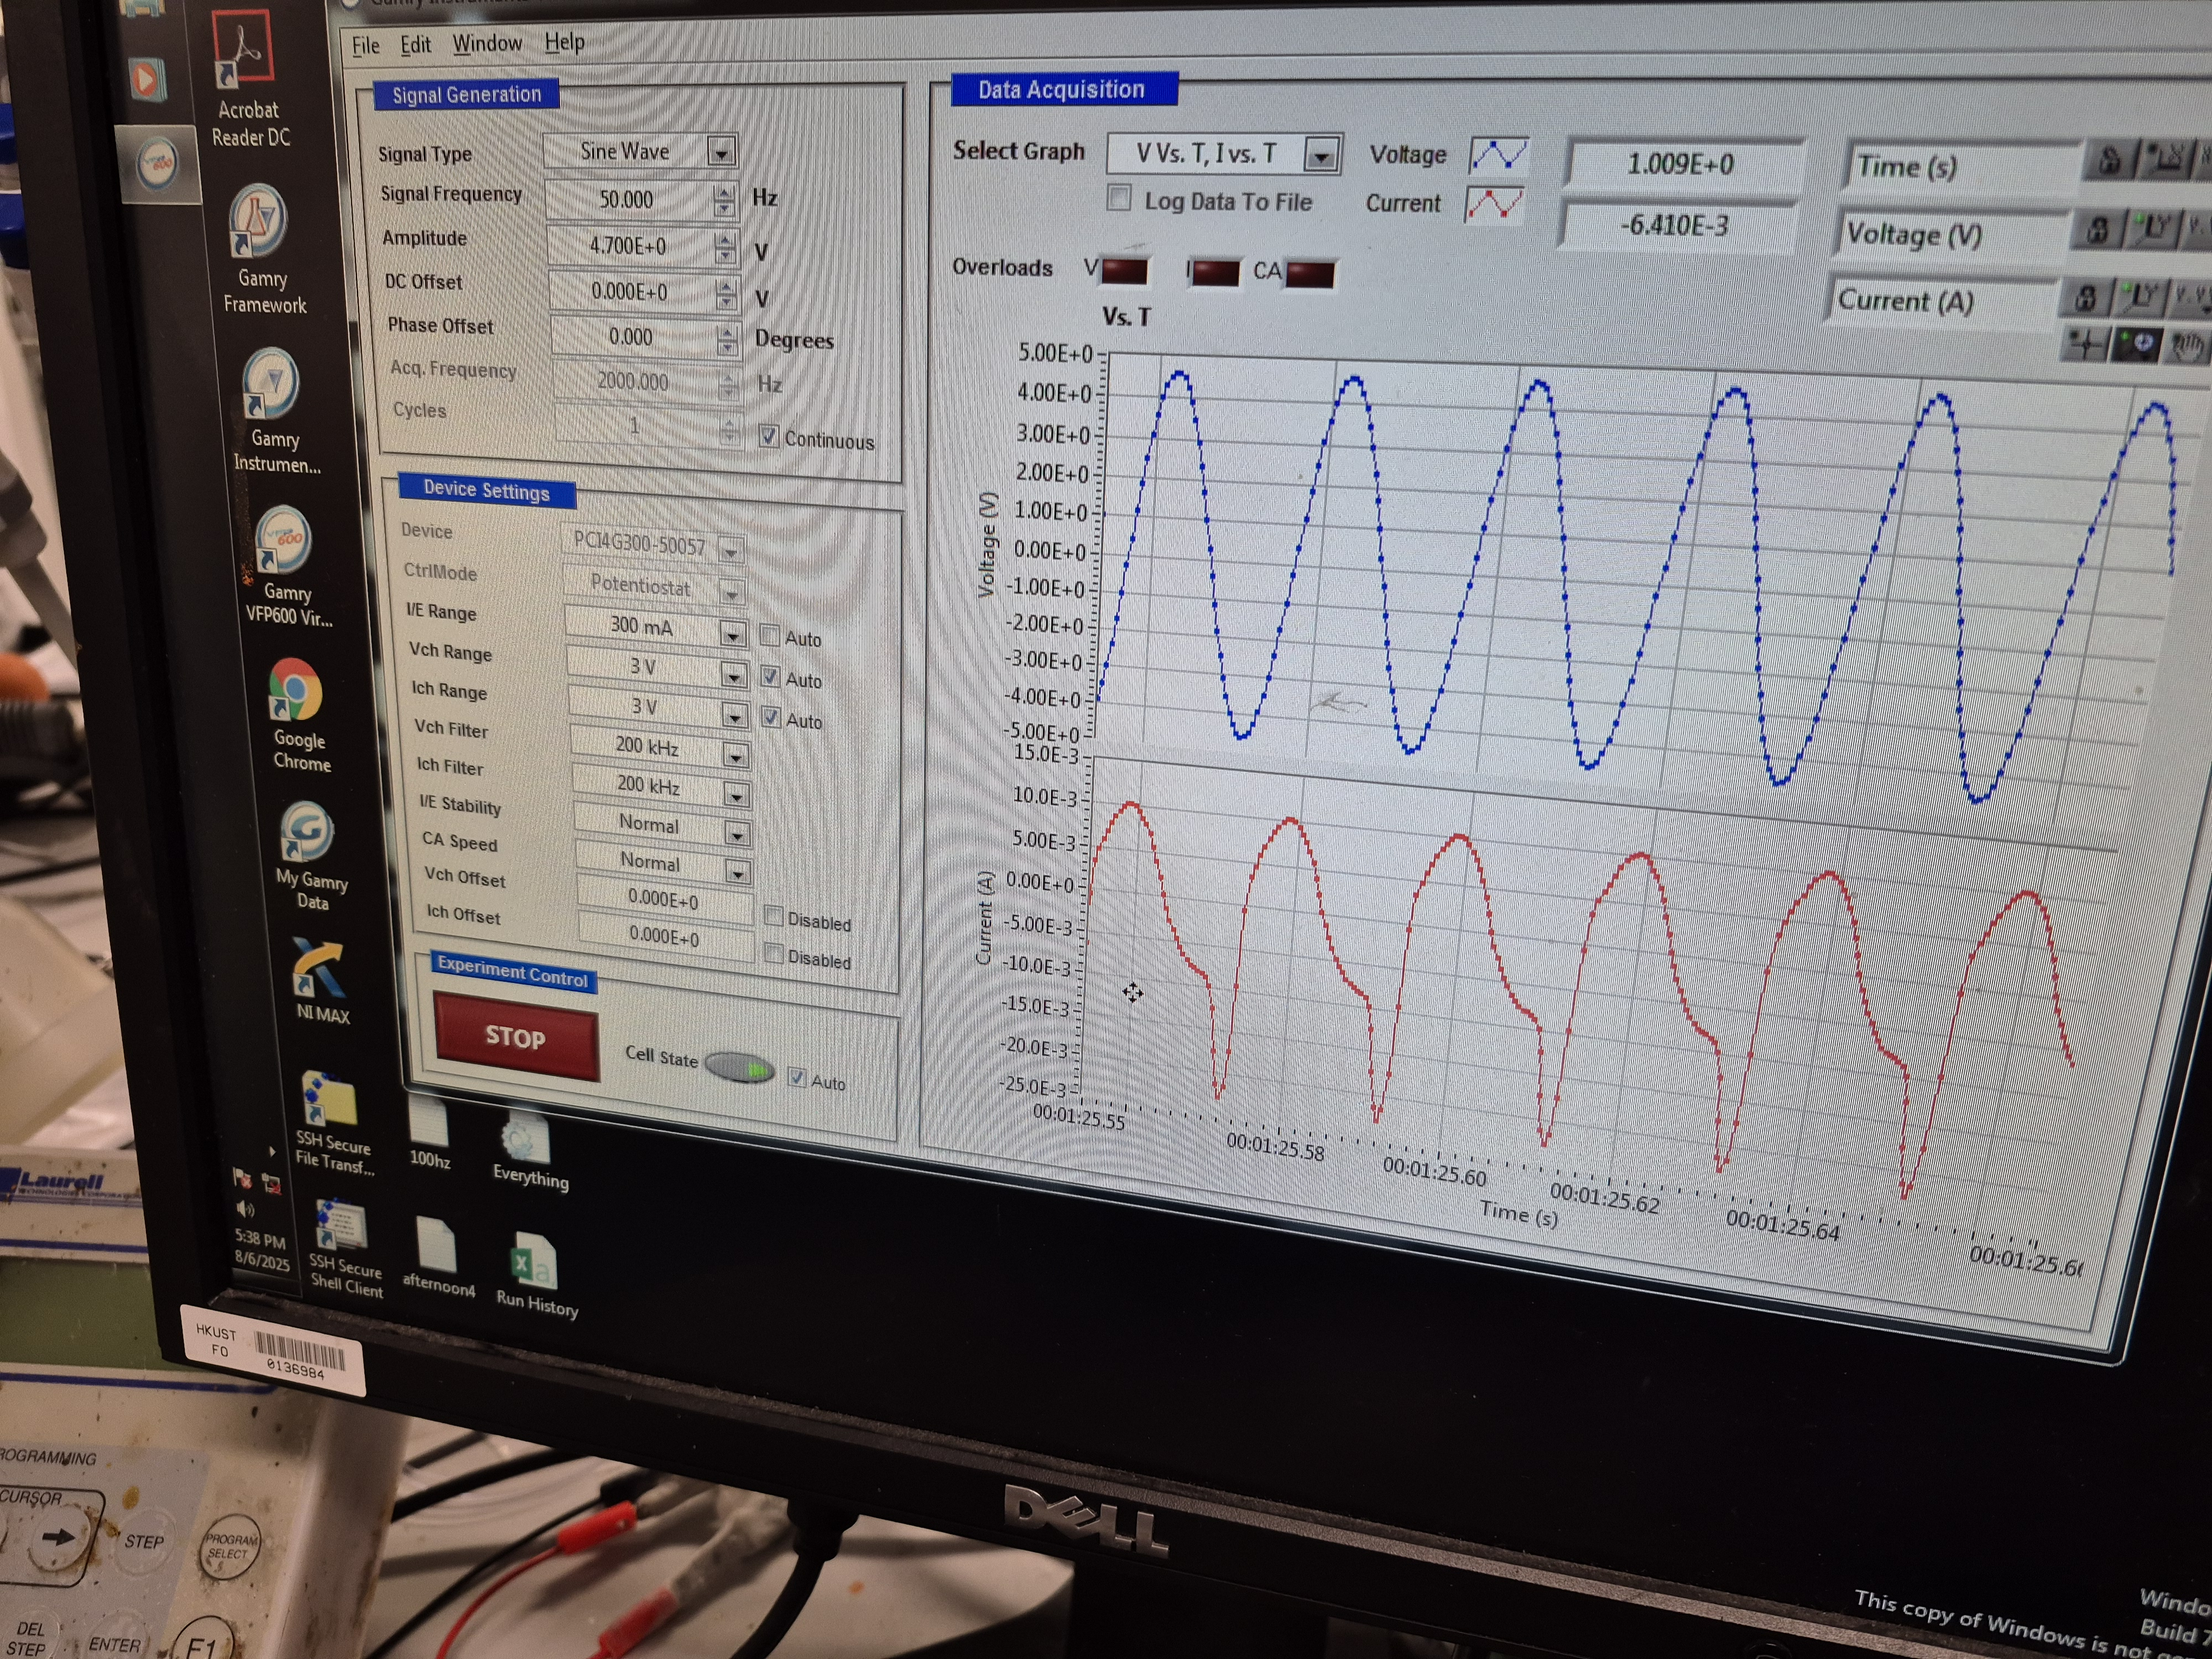
\includegraphics[width=\textwidth]{imgs/EDp.jpg}
			\caption{Pb Electrodeposition Process}
			\label{fig:EDp}
		\end{subfigure}
		\hfill
		%panel (d)
		\begin{subfigure}[b]{0.45\textwidth}
			\centering
			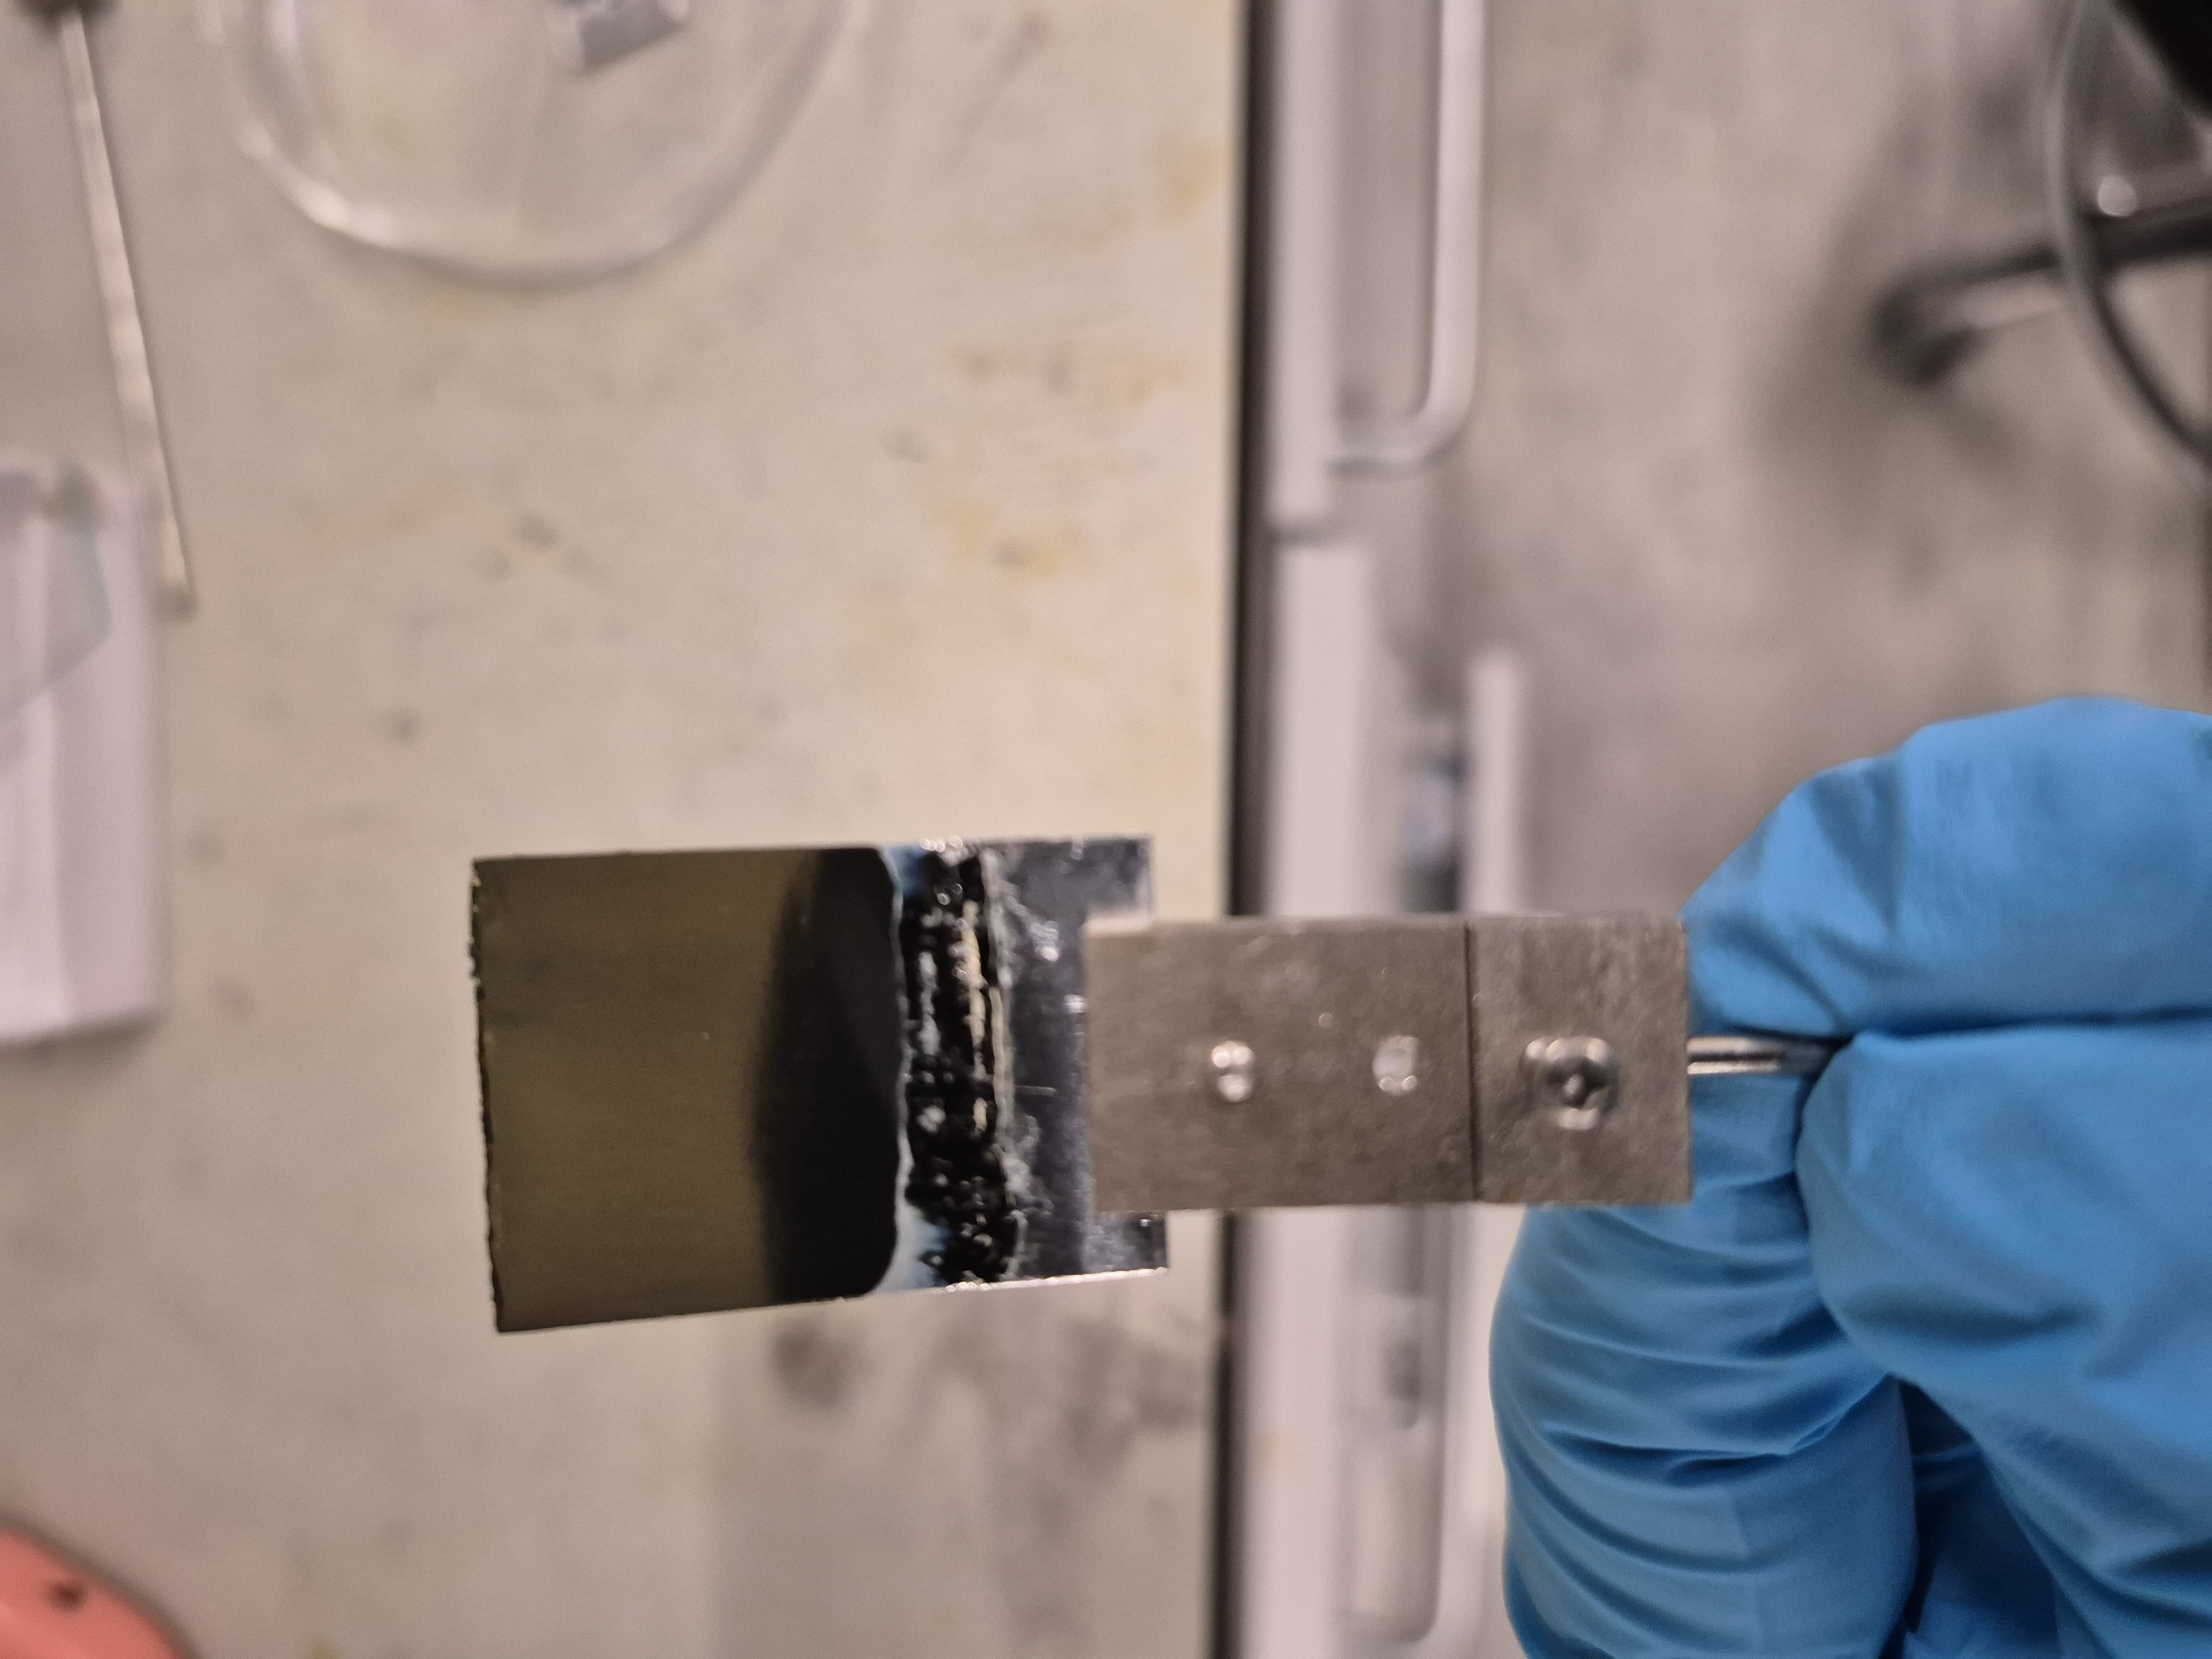
\includegraphics[width=\textwidth,angle=-90]{imgs/EDr.jpg}
			\caption{Pb Electrodeposited PAA}
			\label{fig:EDr}
		\end{subfigure}
		
		\caption{Step-by-step Pb Electrodeposition process.}
		\label{fig:ED}
	\end{figure}
	
	
	
	\subsubsection{CVD process to Grow Nanowires}
	
	Methylammonium iodide (MAI) was synthesized via an acid–base reaction between methylamine and hydroiodic acid. In a $250$ mL three-neck flask cooled to $0~^{\circ}C$, $27.8$ mL of methylamine ($33$ wt\% in ethanol, Sigma–Aldrich) was reacted with $30$ mL of hydroiodic acid ($57$ wt\% in water, Sigma–Aldrich) under continuous stirring for $2$ h. Hydroiodic acid was added dropwise to control the reaction rate and minimize local overheating \cite{gu20163d}.
	A white precipitate formed during the reaction was collected using a rotary evaporator at $50~^{\circ}C$. The crude MAI was dissolved in absolute ethanol and reprecipitated by adding diethyl ether to remove residual impurities. The washing–precipitation cycle was repeated several times to ensure high purity. Finally, the purified MAI powder was dried in a vacuum oven at $60~^{\circ}C$ overnight before use \cite{gu20163d}.
	
	The \ce{MAPbI3} nanowires were synthesized through a vapor–solid reaction between \ce{Pb} and \ce{MAI} vapors in a chemical vapor deposition (CVD) system. The process was carried out in a 2 in. two-zone tube furnace (OTF 1200X-II, MTI). MAI powder was placed at the bottom of a $4$ cm $\times~10$ cm glass bottle, while the prepared PAM/Pb chip (mounted on a Si substrate) was fixed at the bottle opening \cite{gu20163d}.
	
	To enhance vapor confinement, a smaller glass bottle was inserted into the first one, creating an approximately $1$ cm overlap and forming a semi-enclosed environment with elevated MAI vapor pressure. During the growth process, the MAI powder temperature was maintained at $\approx 180~^{\circ}C$, while the PAM/Pb chip region was kept at $205~^{\circ}C$. The reaction proceeded for $6$ h under atmospheric pressure with a constant argon flow of $300$ sccm. After growth, the samples were naturally cooled to room temperature under argon protection \cite{gu20163d} (Figure \ref{fig:CVDp}).
	
	
	\begin{figure}[htpb]
		\centering
		% Panel (a)
		\begin{subfigure}[b]{0.45\textwidth}
			\centering
			\includegraphics[width=0.5\textwidth]{imgs/CVDs.jpg}
			\caption{CVD growth of \ce{MAPbI3} nanowires process}
			\label{fig:cvdS}
		\end{subfigure}
		\hfill
		% Panel (b)
		\begin{subfigure}[b]{0.45\textwidth}
			\centering
			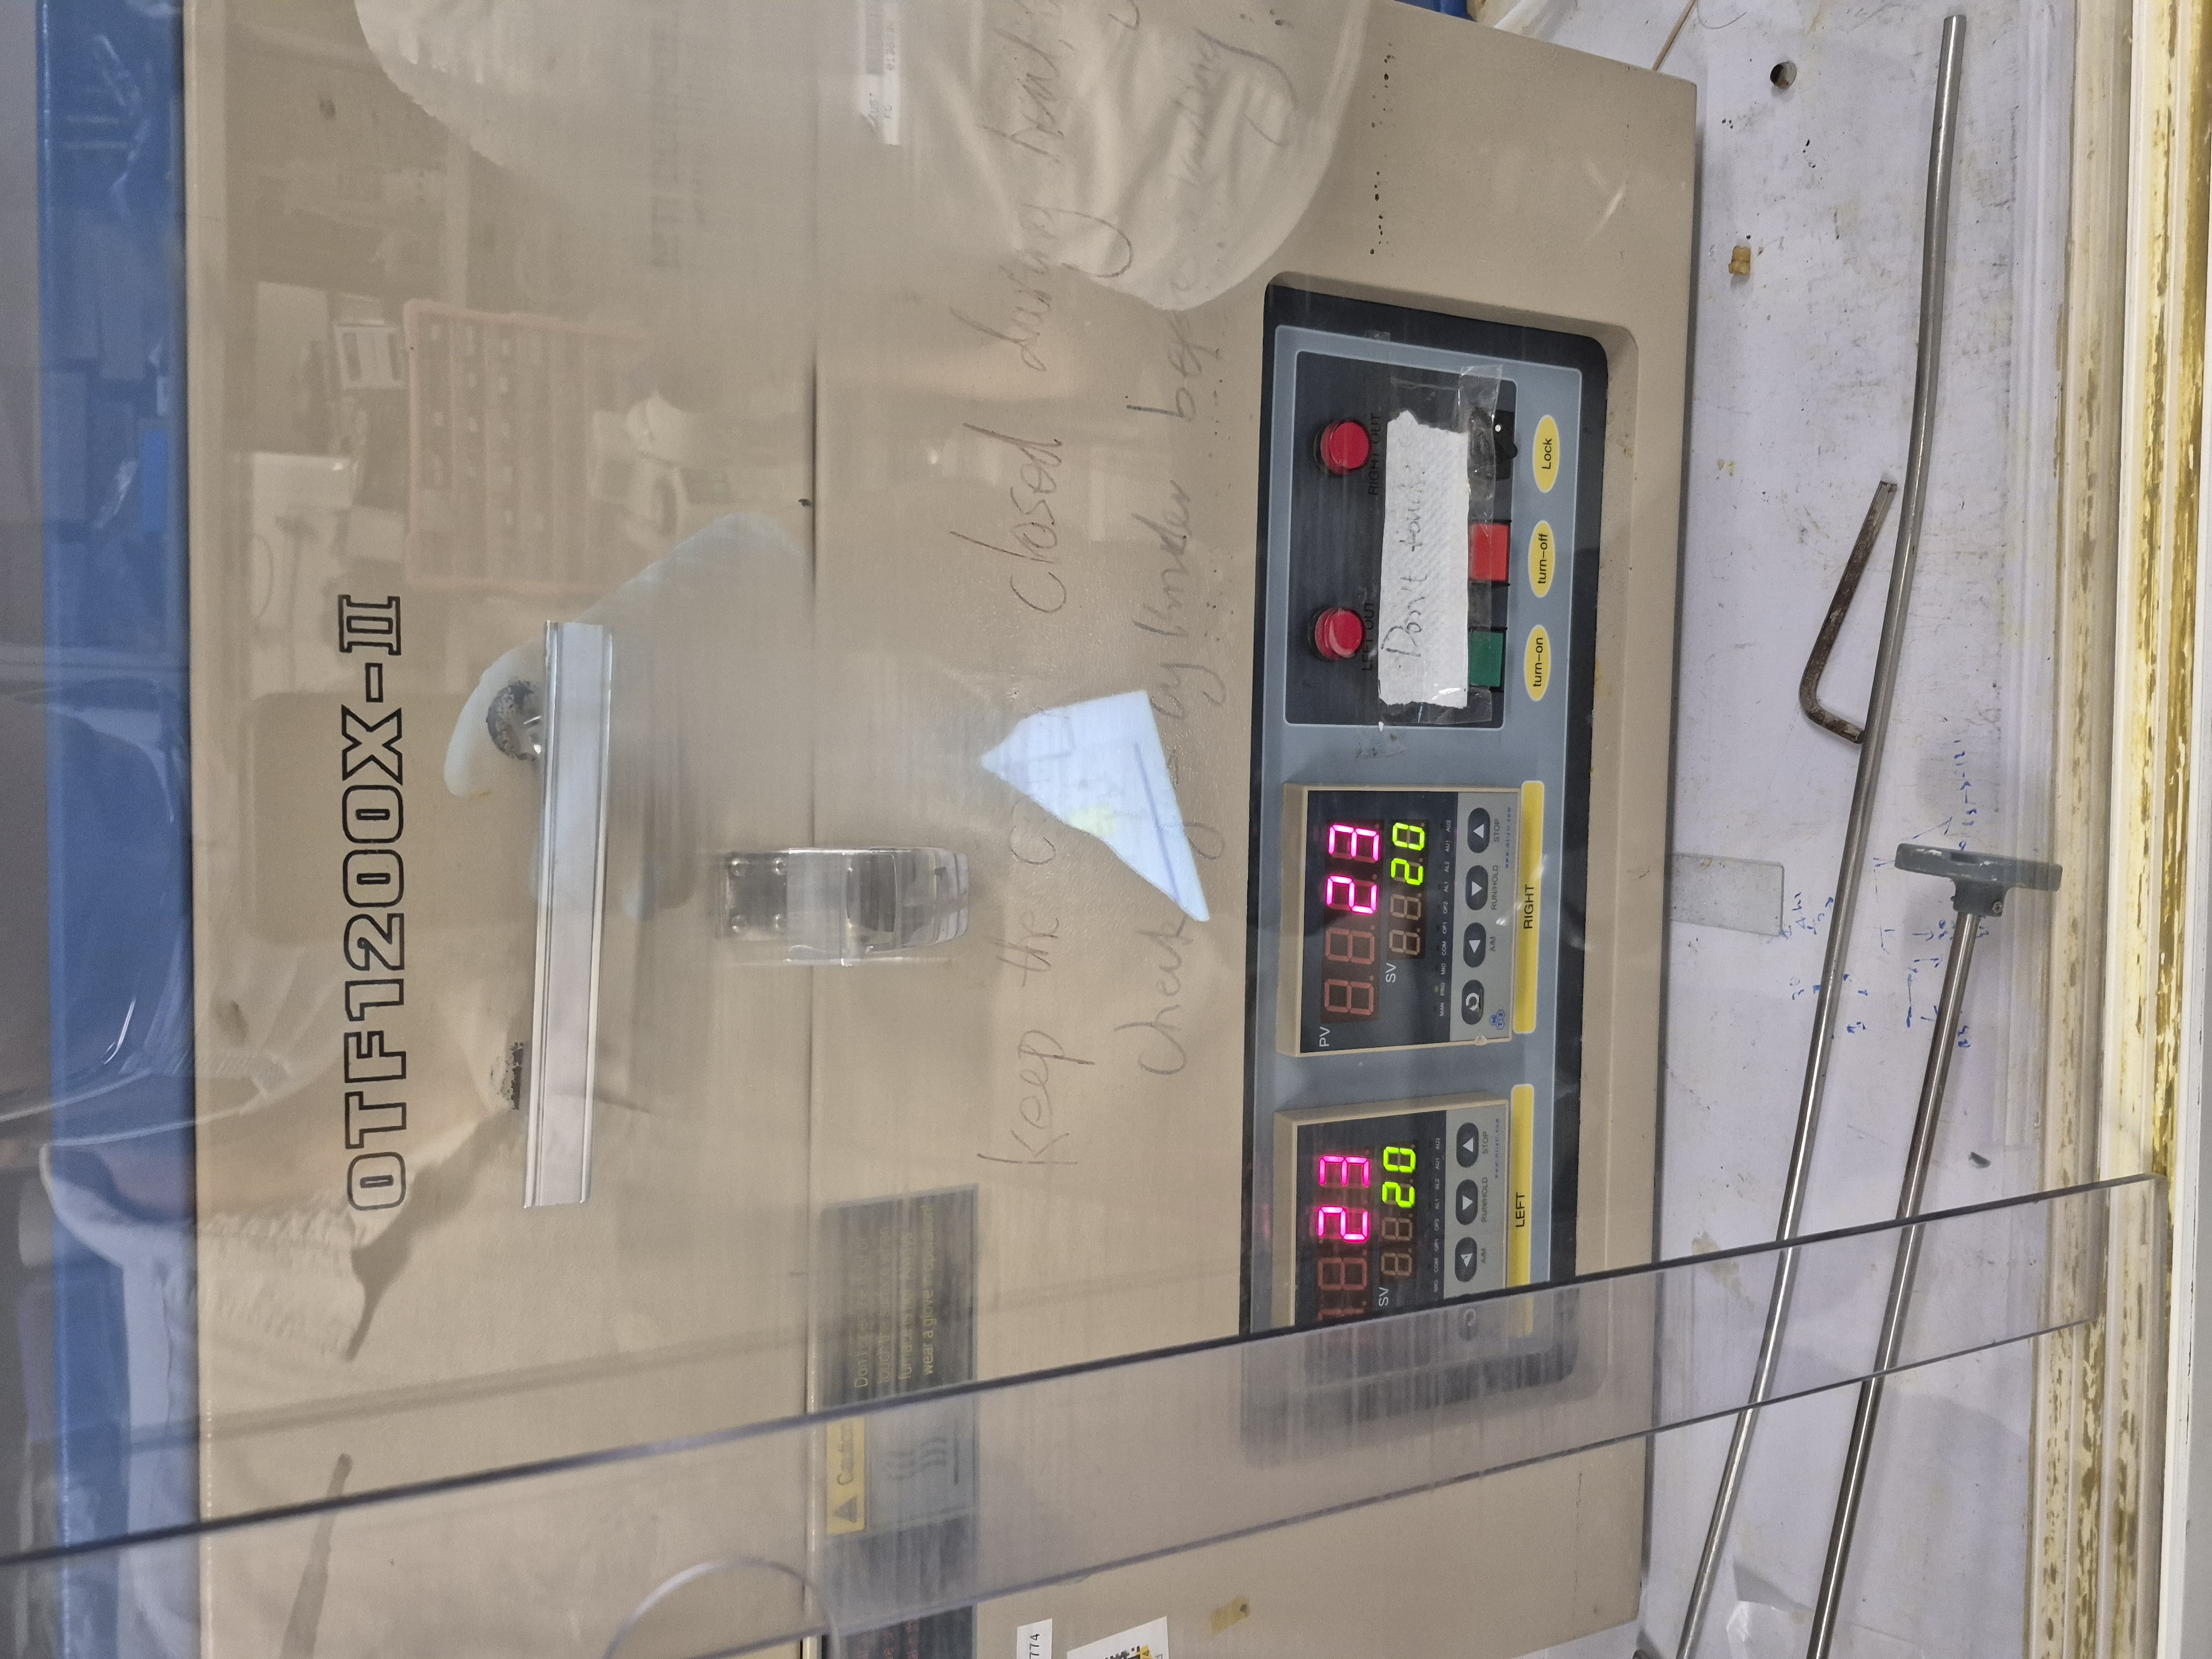
\includegraphics[width=\textwidth, angle=-90]{imgs/CVD.jpg}
			\caption{CVD Process}
			\label{fig:CVD}
		\end{subfigure}
		
		\caption{CVD nanowire growth setting}
		\label{fig:CVDp}
	\end{figure}
	
	
	\subsubsection{Spin-Coating Growth of MAPbBr$_3$ Nanowires}
	
	In an alternative approach to nanowire fabrication, MAPbBr$_3$ nanowires were synthesized through a spin-coating method without the need for prior Pb electrodeposition. After the barrier-thinning step, the porous anodic alumina (PAA) surface was first activated using oxygen plasma treatment for $20$ minutes to improve surface wettability and promote uniform infiltration of the precursor solution (Figure \ref{fig:O2P}).
	
	Subsequently, \ce{a MAPbBr3} precursor solution was dropped onto the plasma-treated PAA surface and left for approximately $2$ minutes to allow the solution to penetrate into the pores via capillary action (Figure \ref{fig:wait}). The substrate was then subjected to spin coating at $2000$ rpm for $30$ seconds to remove the excess solution and ensure a uniform film distribution (Figure \ref{fig:SCf}).
	
	Finally, the sample was annealed at $110~^{\circ}C$ for $10$ minutes to promote solvent evaporation and crystallization of the \ce{MAPbBr3} phase within the pores (Figure \ref{fig:Aneal}). After annealing, the formation of perovskite nanowires inside the PAA template was complete.
	
	\begin{figure}[htpb]
		\centering
		% Panel (a)
		\begin{subfigure}[b]{0.45\textwidth}
			\centering
			\includegraphics[width=\textwidth,angle=-90]{imgs/O2P.jpg}
			\caption{Surface Activation through \ce{O2} plasma}
			\label{fig:O2P}
		\end{subfigure}
		\hfill
		% Panel (b)
		\begin{subfigure}[b]{0.45\textwidth}
			\centering
			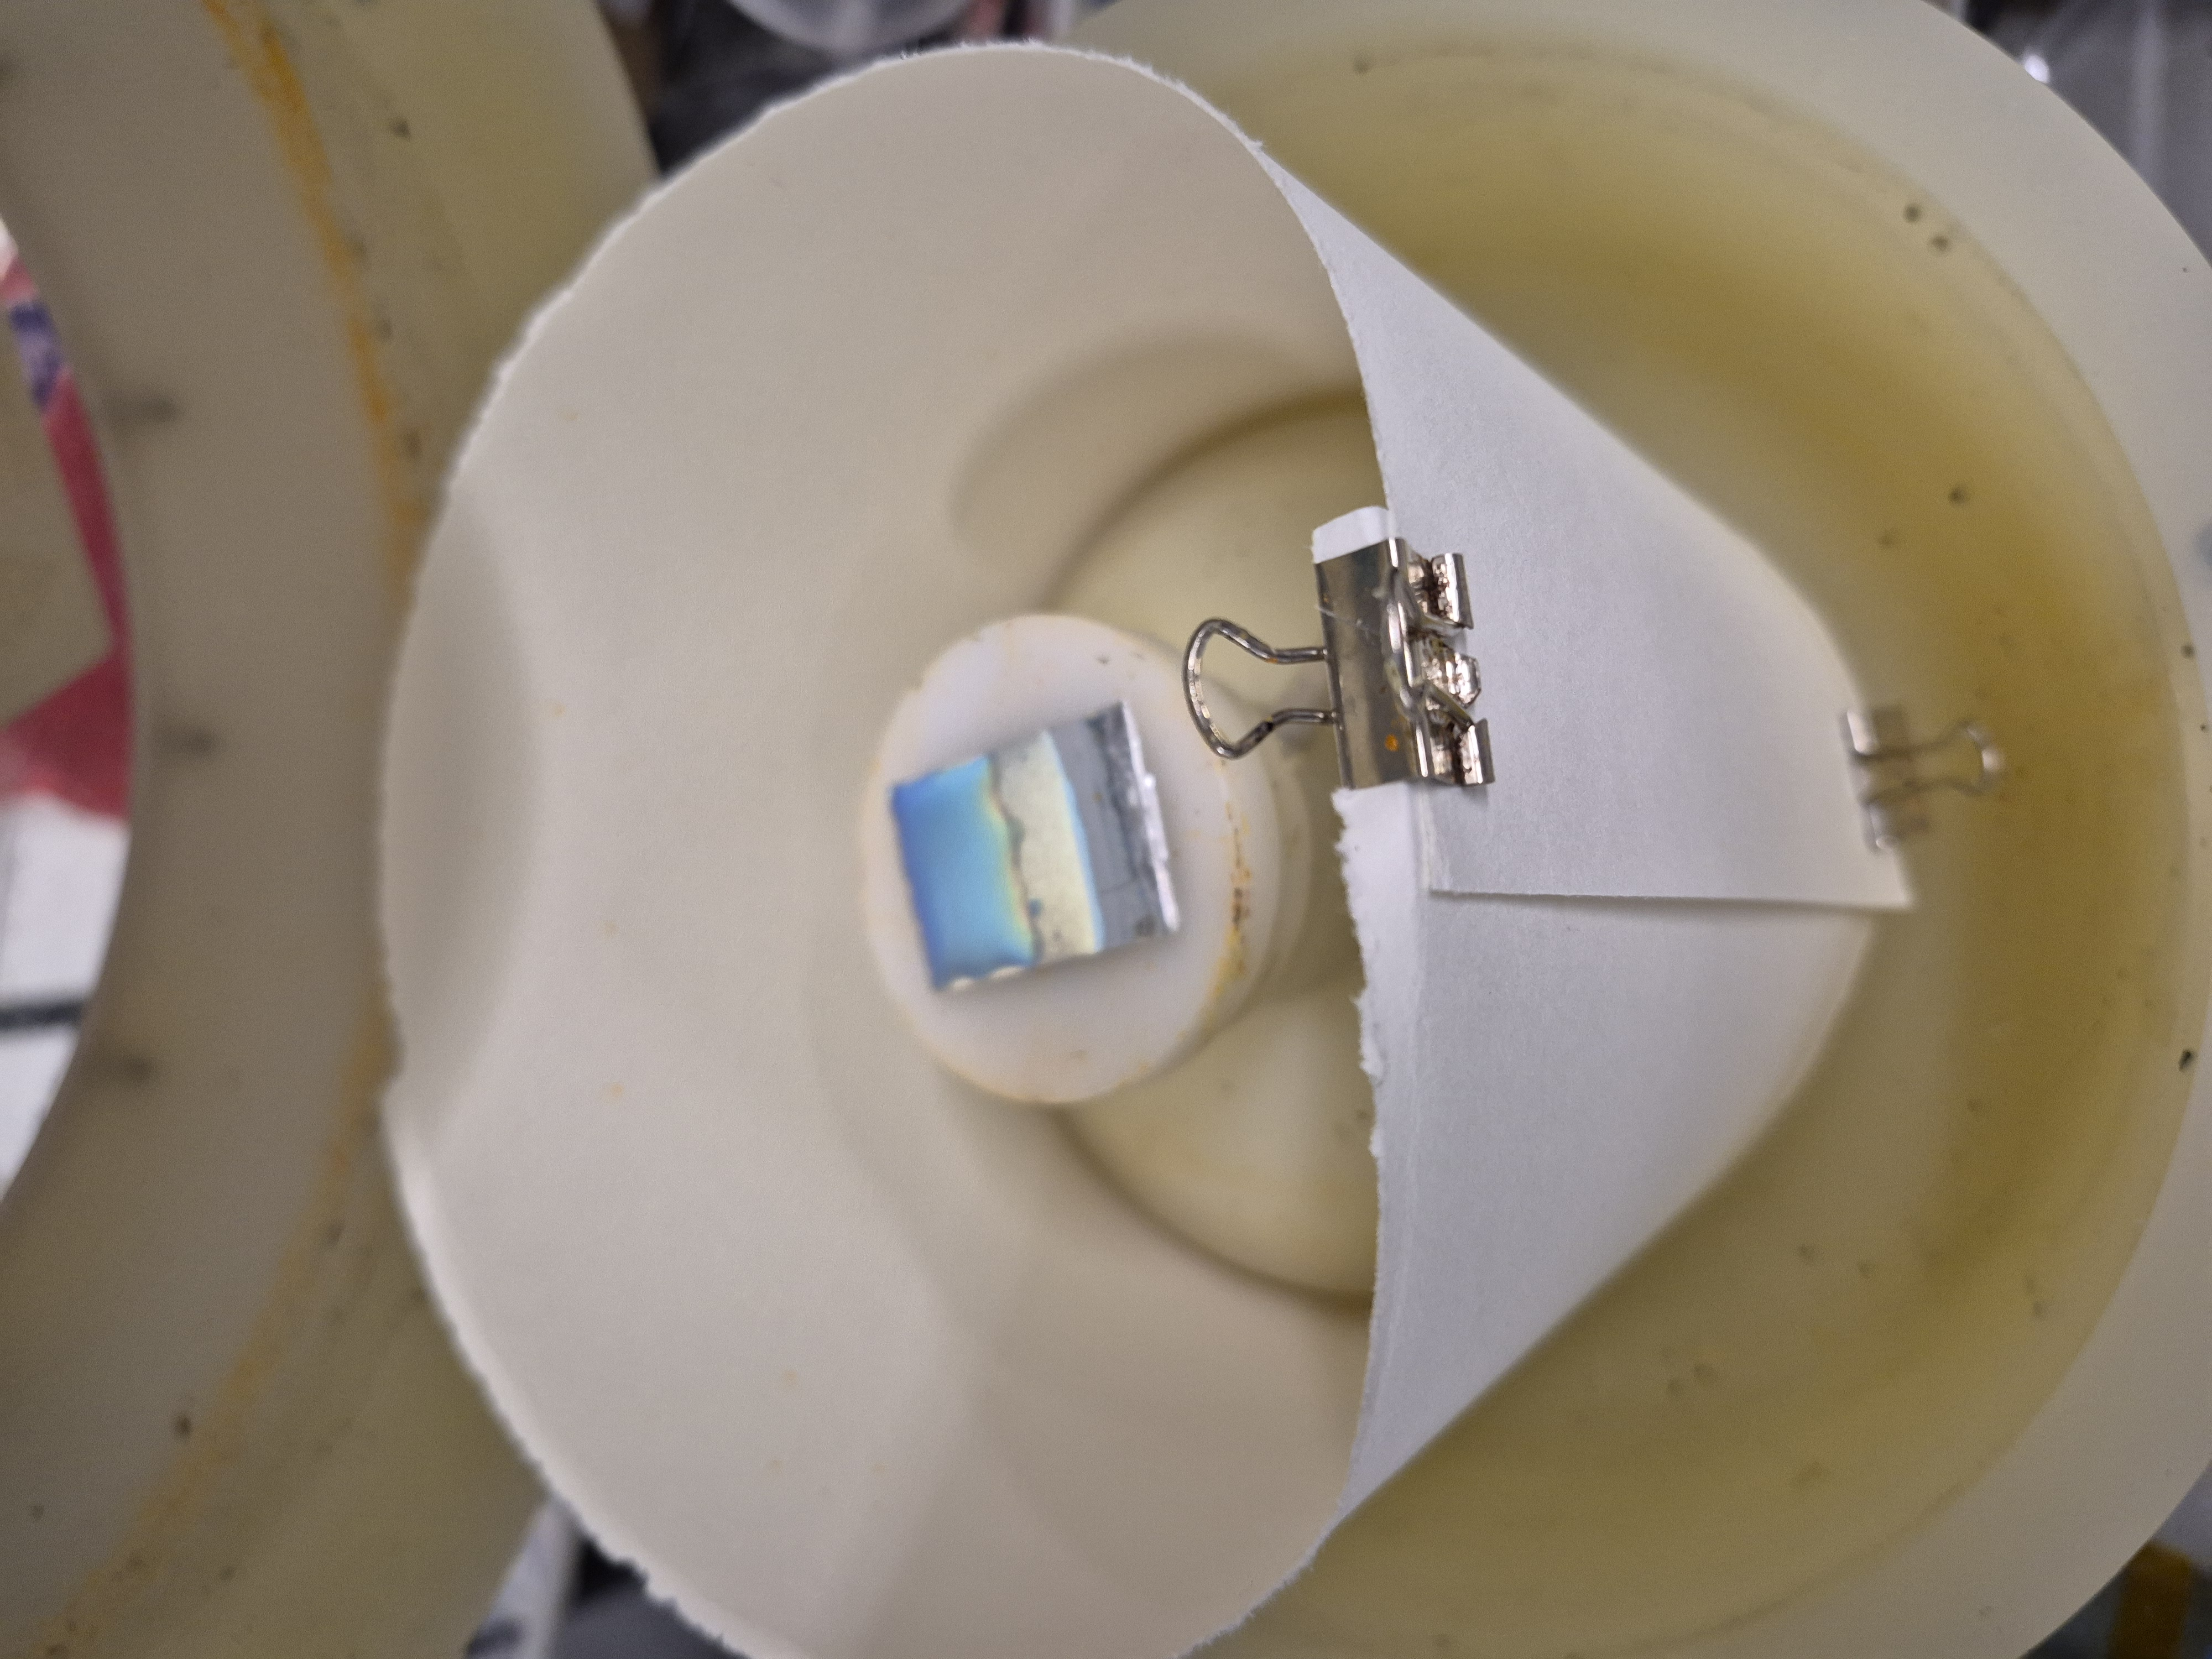
\includegraphics[width=\textwidth,angle=-90]{imgs/wait.jpg}
			\caption{Dropping \ce{MAPbBr3} precursor solution}
			\label{fig:wait}
		\end{subfigure}
		
		\vspace{0.3cm} % optional spacing between rows
		
		% Panel (c)
		\begin{subfigure}[b]{0.45\textwidth}
			\centering
			\includegraphics[width=\textwidth,angle=-90]{imgs/SCf.jpg}
			\caption{PAA after spin coating}
			\label{fig:SCf}
		\end{subfigure}
		\hfill
		%panel (d)
		\begin{subfigure}[b]{0.45\textwidth}
			\centering
			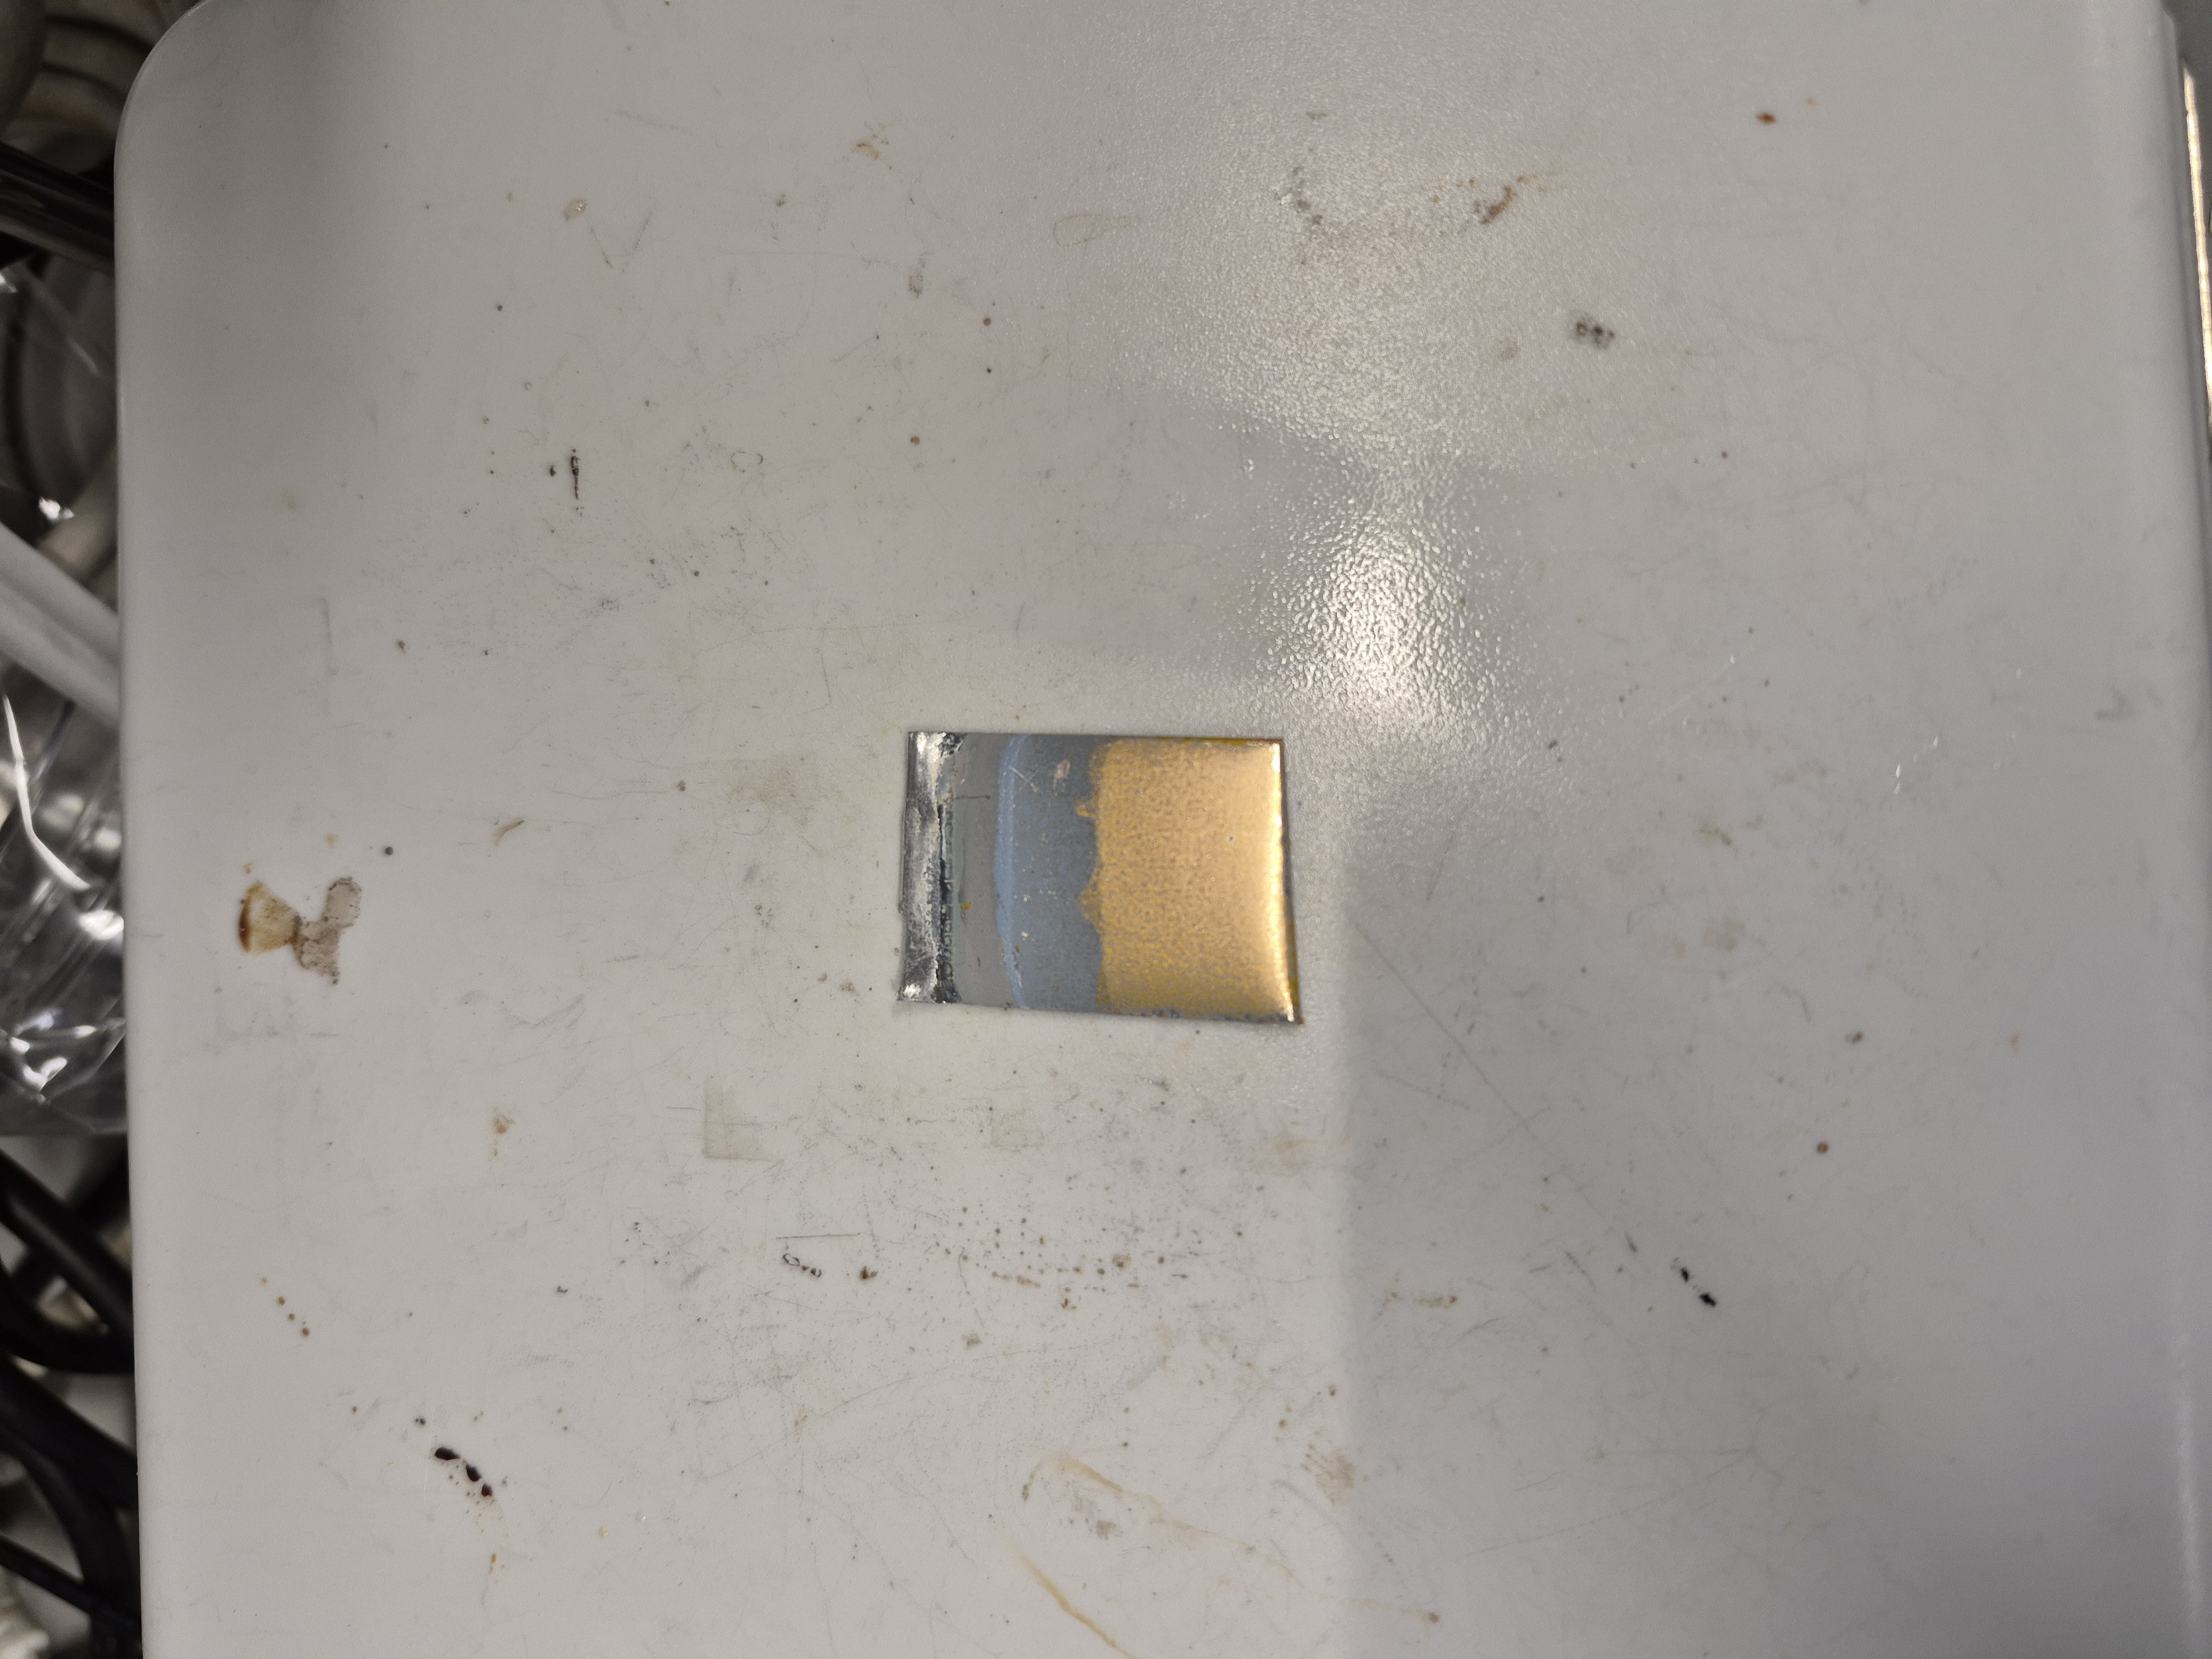
\includegraphics[width=\textwidth,angle=-90]{imgs/Aneal.jpg}
			\caption{Annealing process}
			\label{fig:Aneal}
		\end{subfigure}
		
		\caption{Step-by-step Spin Coating process.}
		\label{fig:SC}
	\end{figure}
	
	\newpage
	\subsubsection{ITO Sputtering for Top Electrode Formation}
	
	After the successful growth of perovskite nanowires within the PAA template, a transparent conducting indium tin oxide (ITO) layer was deposited on top of the filled structure to form the upper electrode of the photodetector device. The deposition was carried out using a magnetron sputtering system under high-vacuum conditions.
	
	A commercially available ITO target was used, and the sputtering power and deposition time were adjusted to achieve an ITO layer thickness of approximately $100 - 150$ nm.
	
	The transparent ITO film serves as the top contact, while the underlying Al substrate functions as the bottom electrode through the thinned barrier layer. This configuration enables vertical carrier transport through the perovskite nanowires embedded in the PAA matrix, completing the photodetector structure (Figure \ref{fig:pd}).
	
	\begin{figure}[htpb]
		\centering
		% Panel (a)
		\begin{subfigure}[b]{0.45\textwidth}
			\centering
			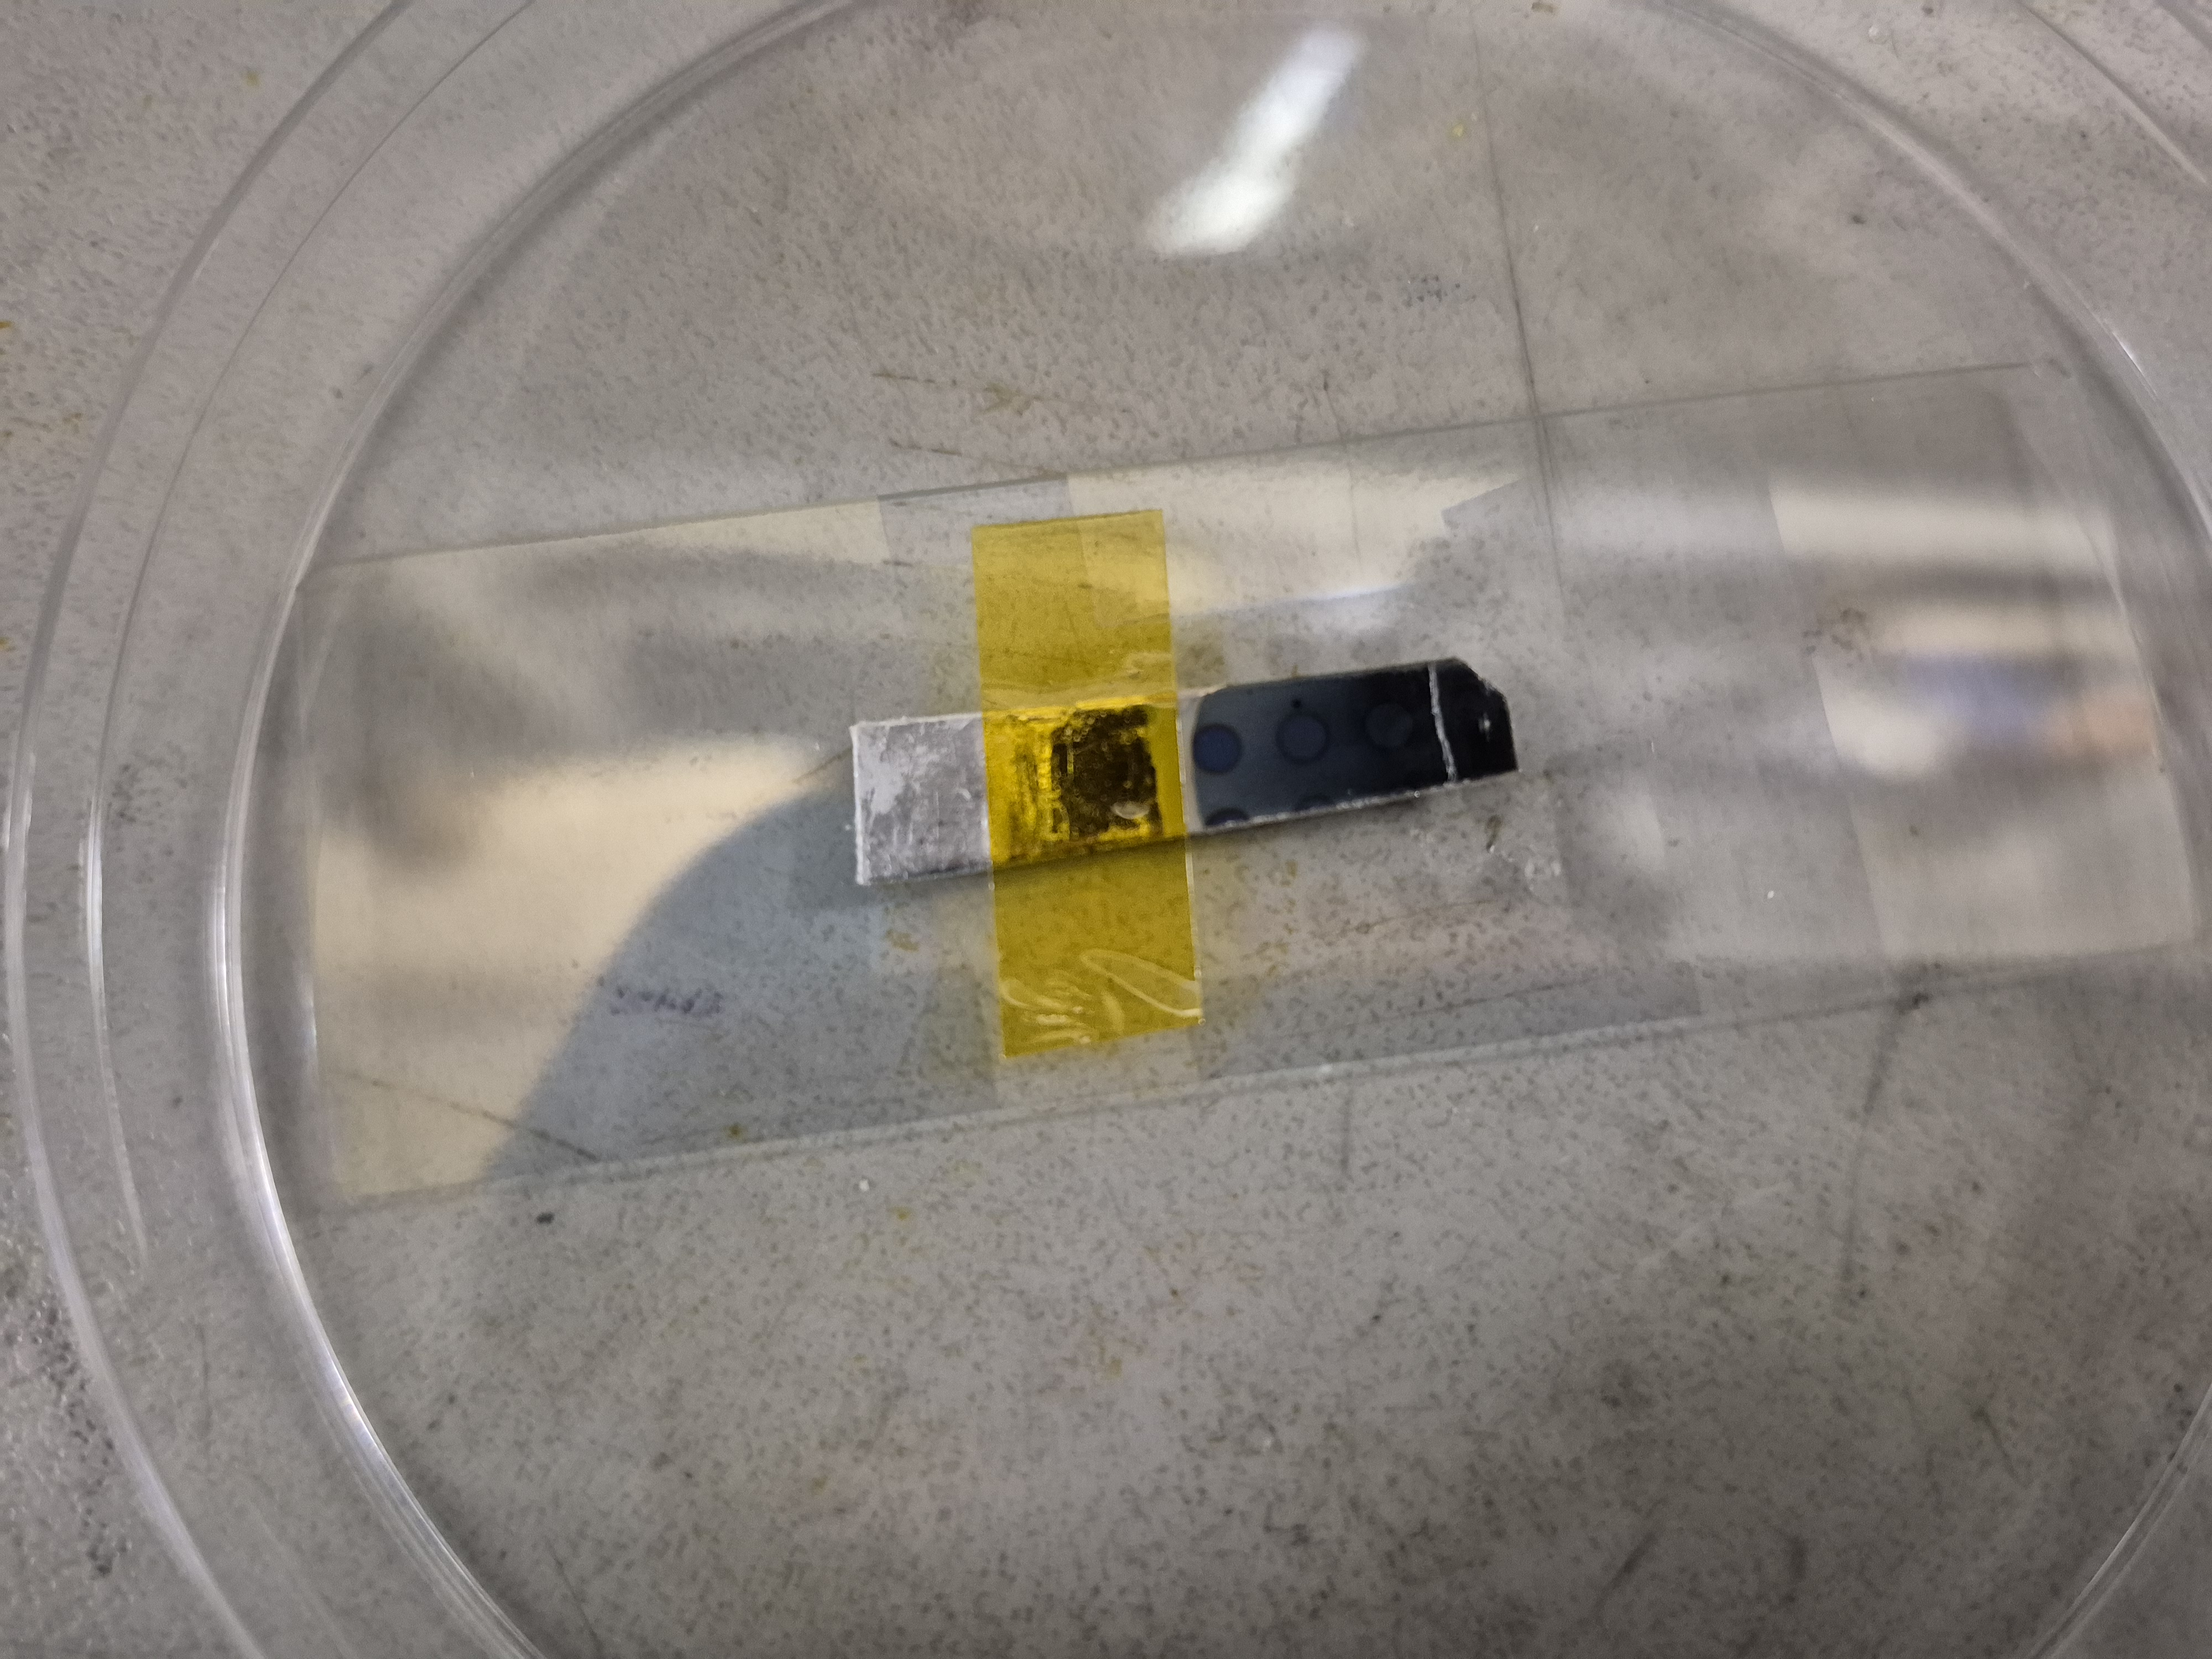
\includegraphics[width=\textwidth]{imgs/CVDpd.jpg}
			\caption{Complete CVD photo detector}
			\label{fig:CVDpd}
		\end{subfigure}
		\hfill
		% Panel (b)
		\begin{subfigure}[b]{0.45\textwidth}
			\centering
			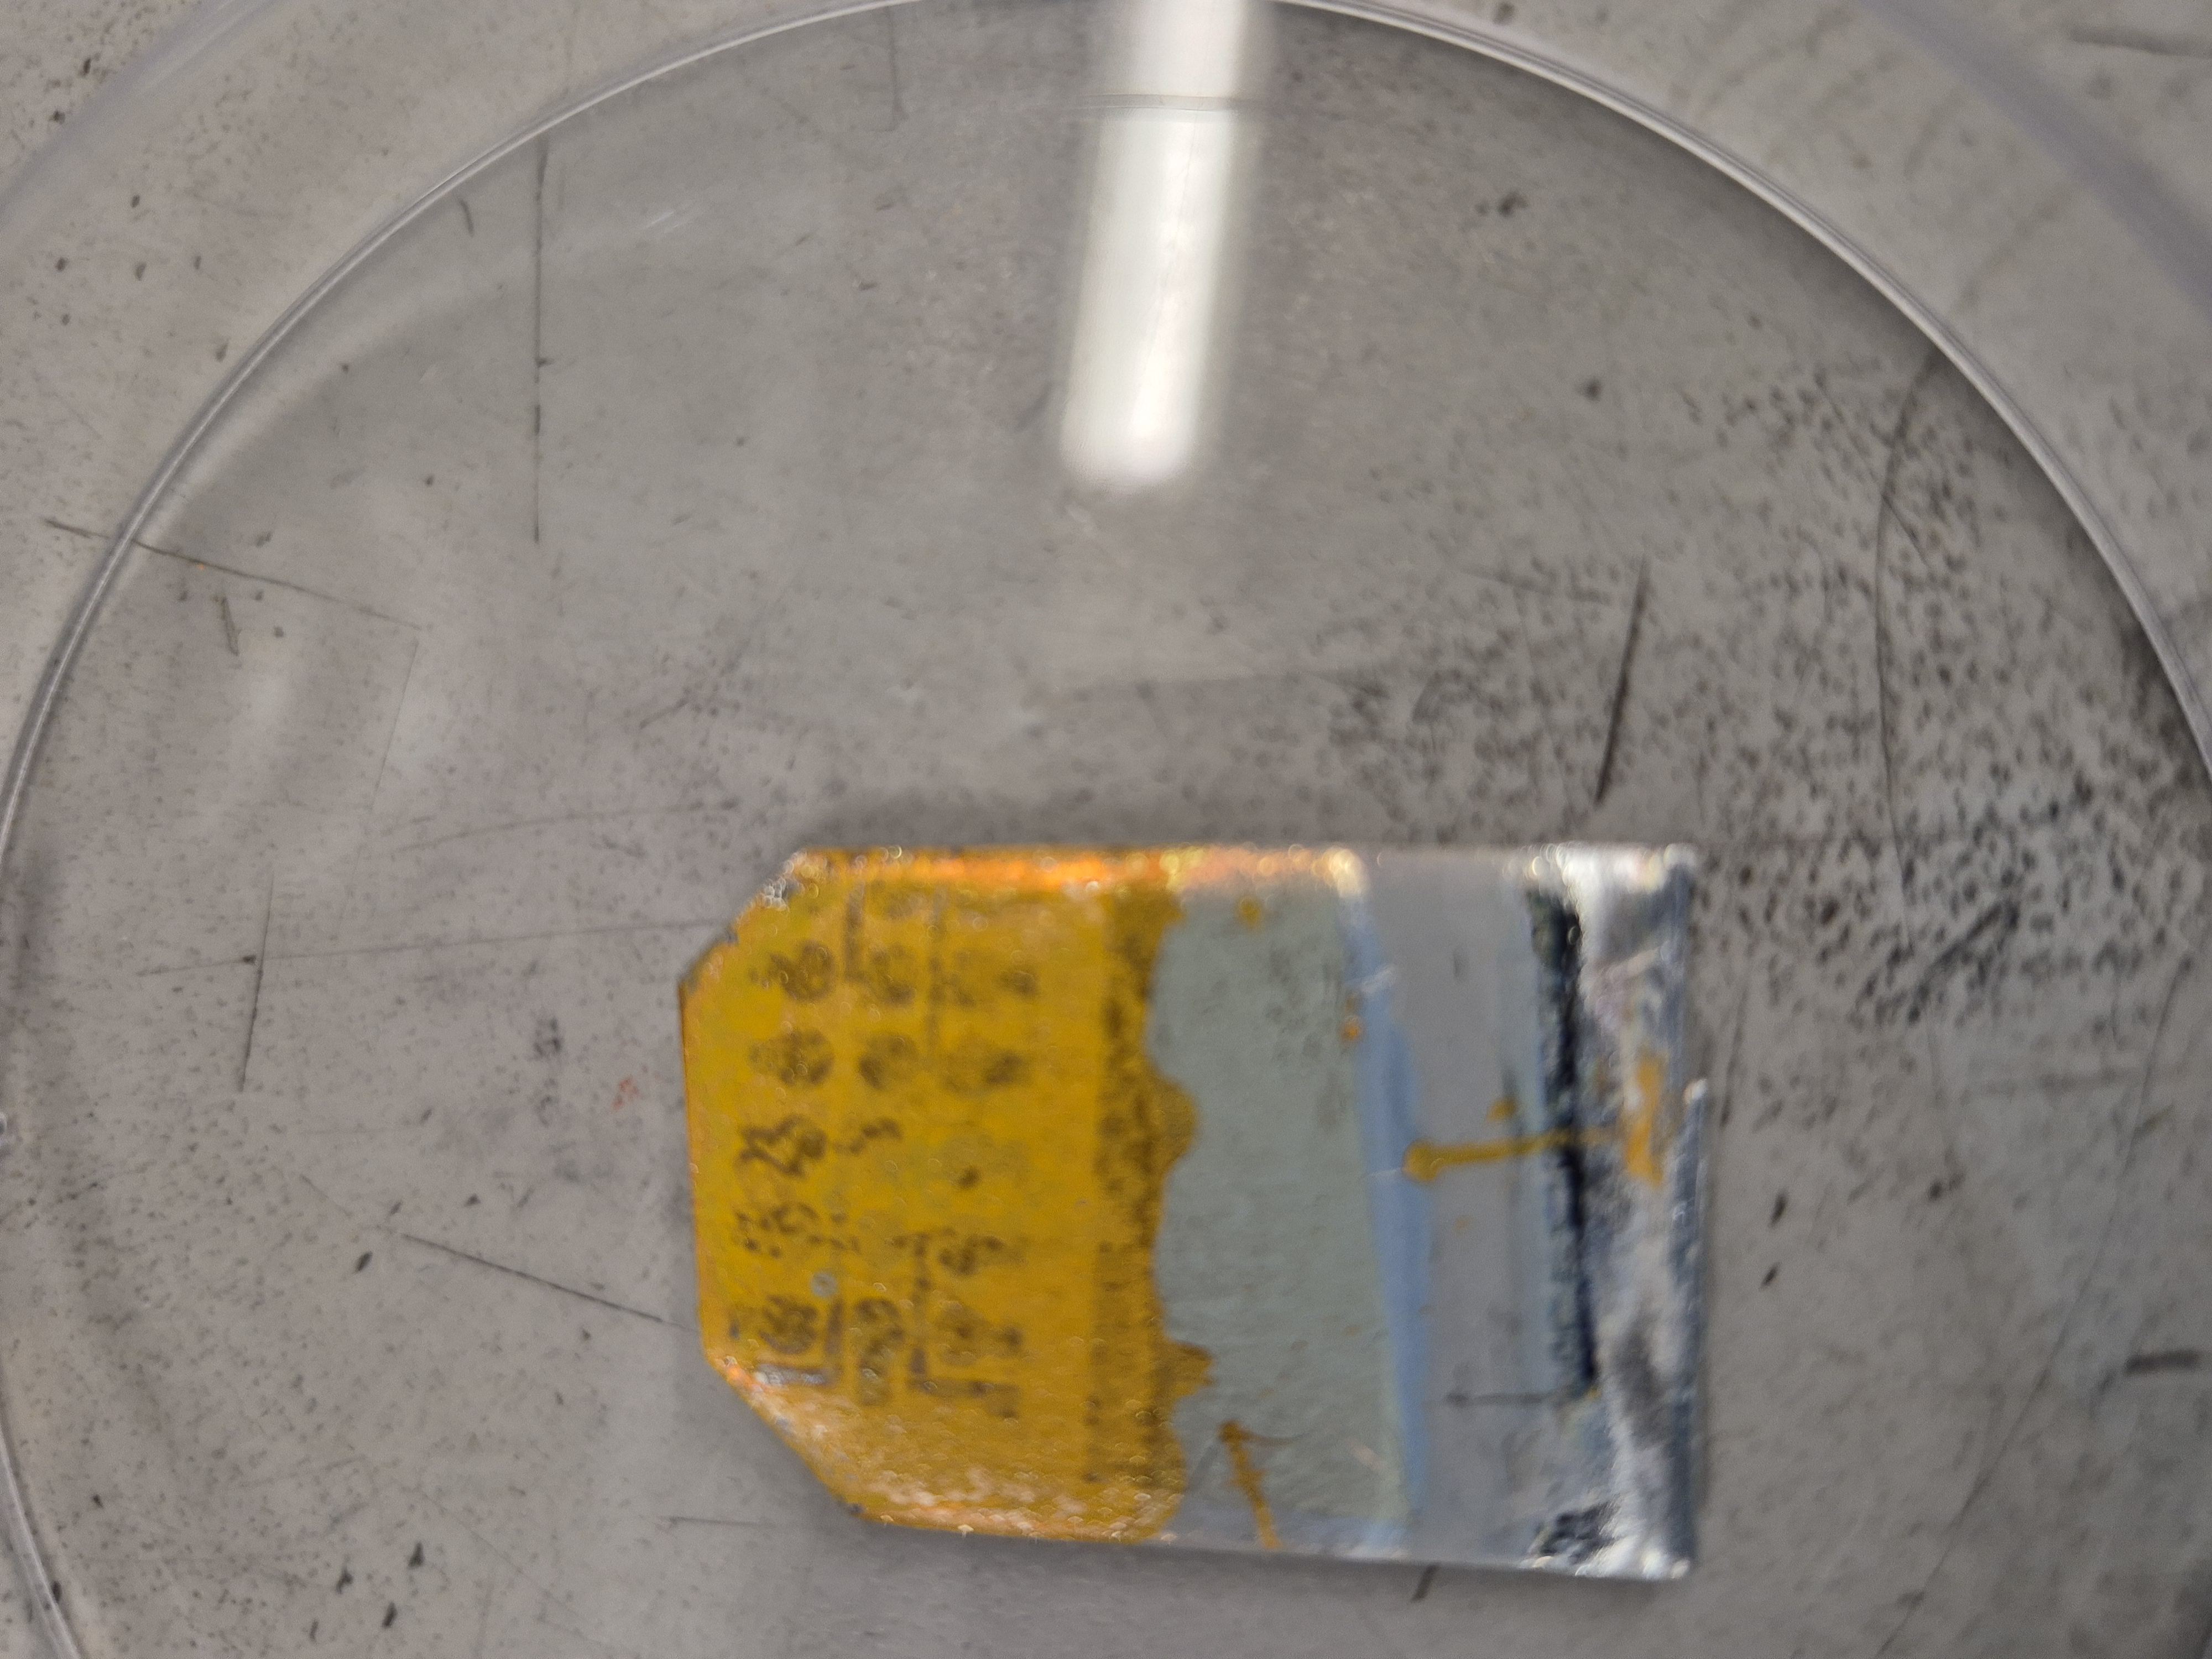
\includegraphics[width=\textwidth]{imgs/SCpd.jpg}
			\caption{Complete spin coated photo detector }
			\label{fig:SCpd}
		\end{subfigure}
		
		\vspace{0.3cm} % optional spacing between rows
		
		% Panel (c)
		\begin{subfigure}[b]{0.45\textwidth}
			\centering
			\includegraphics[width=\textwidth,angle=-90]{imgs/SCpd2.jpg}
			\caption{Another complete spin coated photo detector}
			\label{fig:SCpd2}
		\end{subfigure}
		
		\caption{Complete photo detectors}
		\label{fig:pd}
	\end{figure}
	
	\subsection{Electrical Measurements}
	
	The electrical characterization of the fabricated photodetectors was carried out using an Agilent B1500A Semiconductor Device Analyzer connected to a probe station. Both current–voltage (I–V) and current–time (I–T) measurements were performed under dark and illuminated conditions to evaluate the device performance.
	
	The probe station was equipped with three micromanipulated probe needles and an integrated optical microscope for precise alignment. The photodetector pixel was positioned under the microscope, and two of the probes were carefully placed on the indium tin oxide (ITO) and aluminum (Al) electrodes of the device to form electrical contacts. These probes were then connected to the measurement units of the Agilent analyzer. The microscope’s illumination source served as the light source during the measurements; illumination was controlled simply by switching the microscope light on and off.
	
	To ensure accurate dark measurements and to minimize the influence of ambient light, a light-tight cap was used to cover the probe station during the experiments. The I–V sweeps were performed to examine the current response as a function of the applied bias voltage, while the I–T measurements were used to monitor the transient photocurrent under light on/off cycles.
	
	\subsection{Data Processing and Analysis}

	The raw electrical measurement data, including I–V and I–T curves, were processed using custom Python scripts. Functions were defined to read the CSV files, remove metadata, and return the clean data for each measurement. This preprocessing ensured consistency and facilitated subsequent quantitative analyses.

	The cleaned data were first visualized to examine device behavior and identify trends. I–V curves and I–T curves were plotted for initial inspection. From the I–T measurements, the photocurrent ($I_{ph}$) was calculated, followed by the evaluation of key device performance metrics, including responsivity ($R$) and specific detectivity ($D^{\ast}$), assuming shot-noise-limited conditions.

	The incident light power was measured for each test, and the corresponding light intensity was calculated. For each intensity, the maximum photocurrent was extracted from the I–T curves. These values were then used to plot the photocurrent, responsivity, and specific detectivity as functions of light intensity, allowing for a detailed assessment of the device response under varying illumination conditions.

	This workflow enabled efficient processing of large datasets, ensuring reproducibility and consistency in the evaluation of the device performance.
	
	\section{Results and Discussion}
	
	\subsection{Nanowire Growth via Spin Coating}
	
	The perovskite nanowires fabricated by the spin coating method exhibit a highly uniform and vertically aligned morphology that closely follows the geometry of the PAA nanochannels. Owing to the capillary infiltration of the \ce{MAPbBr3} precursor solution into the ordered pores, the nanowires inherit the diameter and arrangement defined by the anodic alumina template, typically in the range of $200$ nm.
	
	Compared to vapor-phase growth, the spin-coated nanowires generally show smoother surfaces and more homogeneous filling across the template area, though partial pore filling can occur if the precursor infiltration is incomplete. The short infiltration time and moderate spinning speed facilitate uniform distribution while preventing excessive accumulation on the surface.
	
	Post-annealing at 1$110~^{\circ}C$ promotes solvent evaporation and crystallization of the perovskite phase, leading to well-defined one-dimensional nanostructures with high crystallinity. The nanowires are typically single crystalline or contain large crystalline domains, as the confined pore environment favors oriented growth along the pore axis. The resulting structure is a dense, vertically aligned nanowire array embedded within the PAA matrix, suitable for optoelectronic applications such as photodetectors and light-emitting devices.
	
	\subsubsection{SEM images of the Spin Caoted Photo Detector}
	
	\begin{figure}[htpb]
		\centering
		% Panel (a)
		\begin{subfigure}[b]{0.45\textwidth}
			\centering
			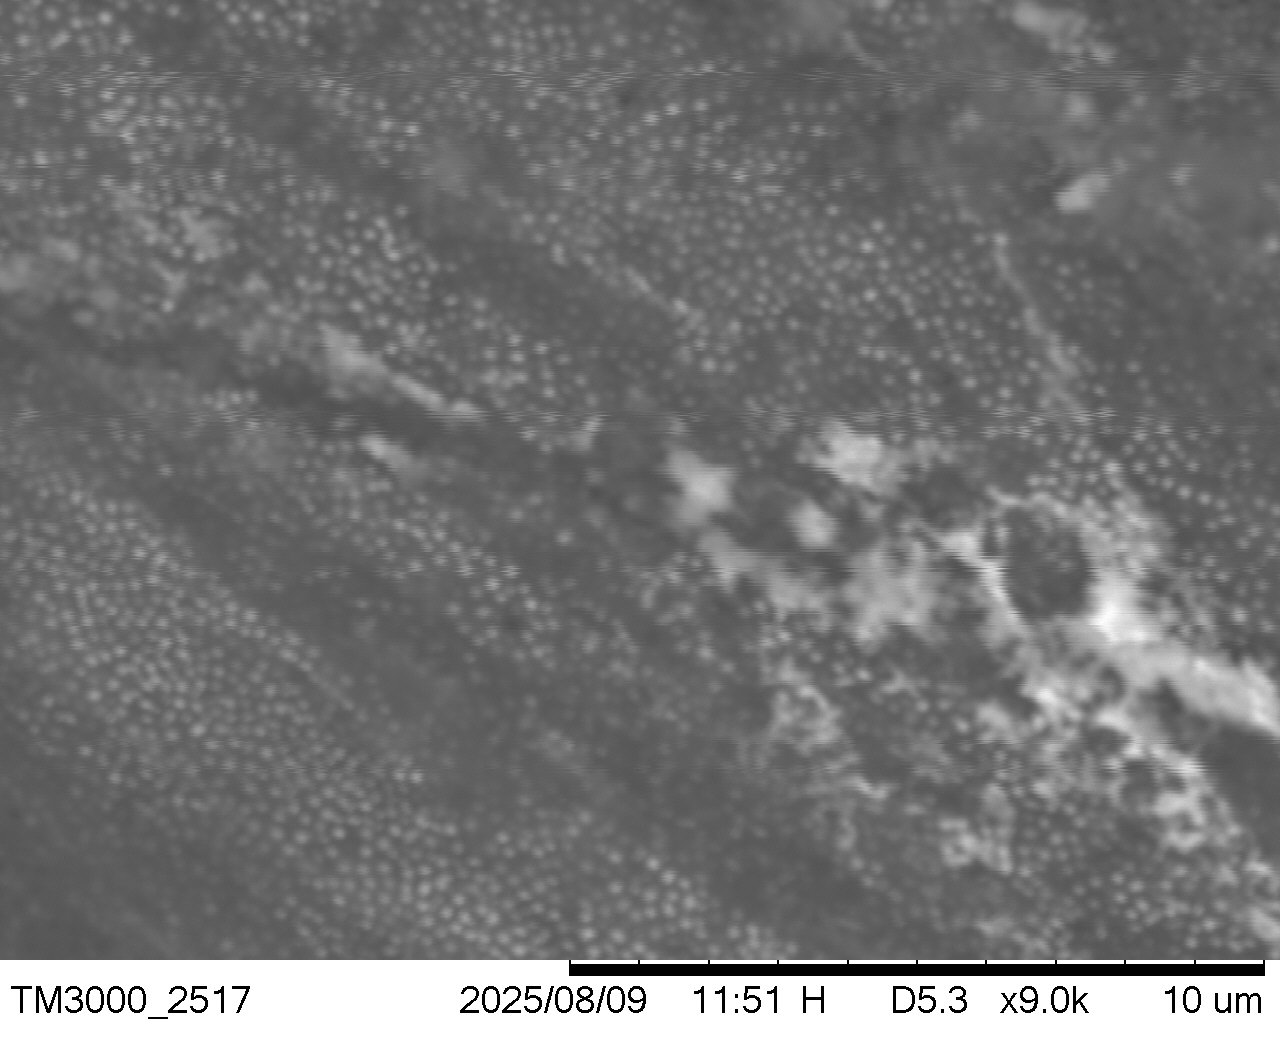
\includegraphics[width=\textwidth]{imgs/4.jpg}
			\caption{Top view SEM of the spin coated photo detector}
			\label{fig:TVSCpd}
		\end{subfigure}
		\hfill
		% Panel (b)
		\begin{subfigure}[b]{0.45\textwidth}
			\centering
			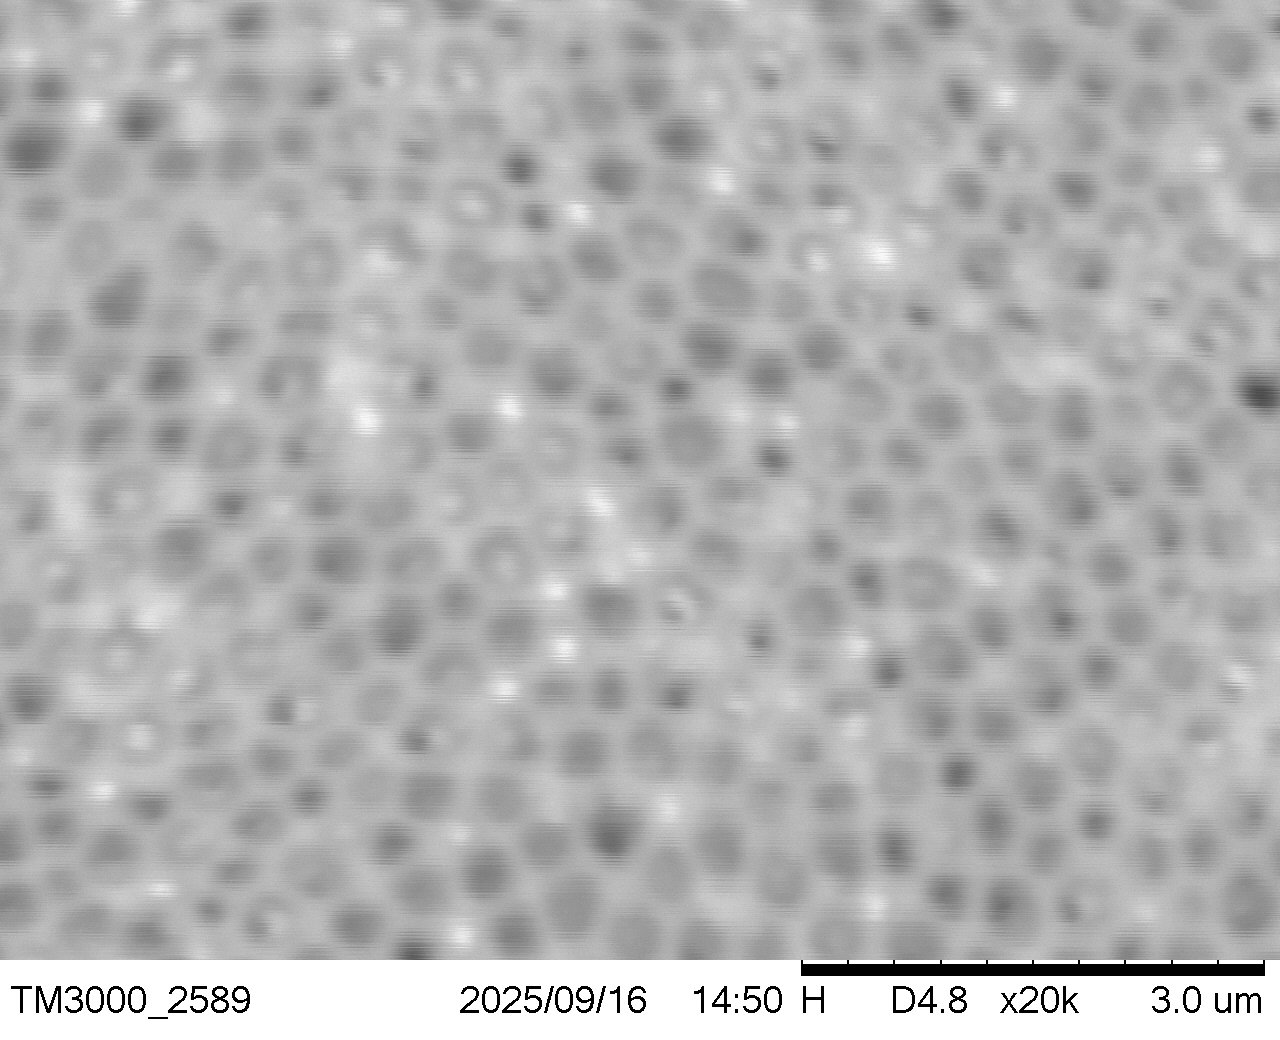
\includegraphics[width=\textwidth]{imgs/2.jpg}
			\caption{Top view SEM of the spin coated photo detector }
			\label{fig:TVSCpd2}
		\end{subfigure}
		
		\vspace{0.3cm} % optional spacing between rows
		
		% Panel (c)
		\begin{subfigure}[b]{0.45\textwidth}
			\centering
			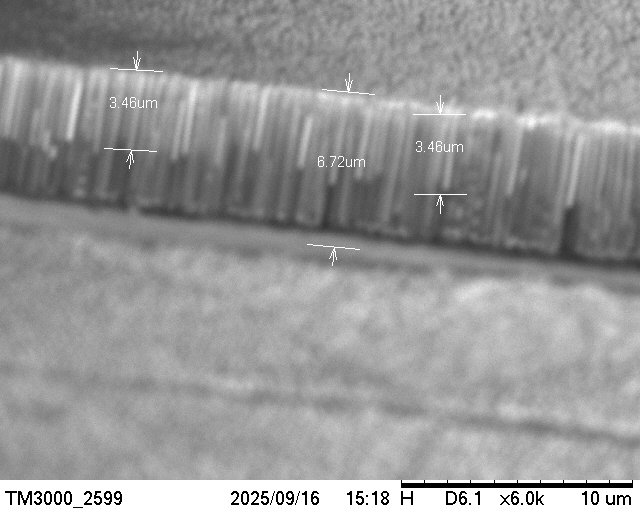
\includegraphics[width=\textwidth]{imgs/12.jpg}
			\caption{Cross section view SEM of the spin coated photo detector}
			\label{fig:CVSCpd}
		\end{subfigure}
		
		\caption{SEM images of the spin coated photo detector}
		\label{fig:SEMSCpd}
	\end{figure}
	
	
	The SEM images in Figure \ref{fig:SEMSCpd} demonstrate that the \ce{MAPbBr3} nanowires fabricated via the spin-coating method were successfully formed within the porous anodic alumina (PAA) template. The top-view SEM (Figure \ref{fig:TVSCpd2}) reveals a highly ordered hexagonal arrangement of pore openings with uniform diameters, confirming that the nanowires replicate the template geometry. The average pore spacing and diameter are consistent across the surface, indicating good wetting and infiltration of the precursor solution after \ce{O2} plasma activation.
	
	The cross-sectional image (Figure \ref{fig:CVSCpd}) shows that the nanowires are vertically aligned and uniformly distributed throughout the pore depth. The measured nanochannel lengths range from approximately up to $6.7 \mu m$, corresponding well with the total pore length of the PAA layer. The nanowires inside the nanochannels seem to be halved due to the cutting process. This suggests effective penetration of the \ce{MAPbBr3} precursor into the nanochannels prior to solvent evaporation during spinning. The nanowires exhibit a columnar morphology with smooth sidewalls, indicating continuous filling and minimal void formation.
	
	In some areas (Figure \ref{fig:TVSCpd}), localized regions of incomplete filling or surface agglomeration can be observed, likely due to uneven solvent evaporation or partial precursor depletion during spin coating. However, the overall array uniformity and vertical alignment are well preserved, highlighting the effectiveness of the oxygen plasma treatment in improving the PAA surface wettability and the infiltration of the perovskite precursor.
	
	
	The \ce{MAPbBr3} nanowires produced via spin coating exhibit a high degree of structural uniformity across the PAA surface. The top-view SEM image shows that the nanowires (replicating the PAA pore arrangement) maintain a consistent hexagonal ordering throughout the scanned area, confirming homogeneous infiltration of the perovskite precursor into the nanochannels. This uniform distribution implies that the precursor concentration, viscosity, and spinning parameters were well balanced to achieve even filling without significant aggregation or clogging at the pore openings.
	
	In terms of coverage, the PAA template appears to be almost completely filled with perovskite material, as evidenced by the bright circular contrasts visible across the surface. Only a few minor regions exhibit incomplete filling or surface residues, possibly caused by local variations in solvent evaporation or precursor retention during the spinning process. The overall coverage can therefore be considered continuous and nearly complete across the entire template area.
	
	The alignment of the nanowires, as seen in the cross-sectional SEM image, is distinctly vertical and uniform over micrometer-scale regions. The nanowires maintain consistent lengths up to  $6.7 \mu m$, following the geometry of the underlying PAA channels. This vertical alignment is inherently guided by the highly ordered pore structure of the anodic alumina template, allowing the perovskite nanowires to grow along the normal direction to the substrate. Such alignment is particularly advantageous for optoelectronic applications, as it facilitates efficient charge transport along the nanowire axes and enhances light–matter interaction due to minimized scattering at the interfaces.
	
	\subsubsection{Photoresponse Behavior: Current-Time Measurements}
	
	\begin{figure}[htpb]
		\centering
		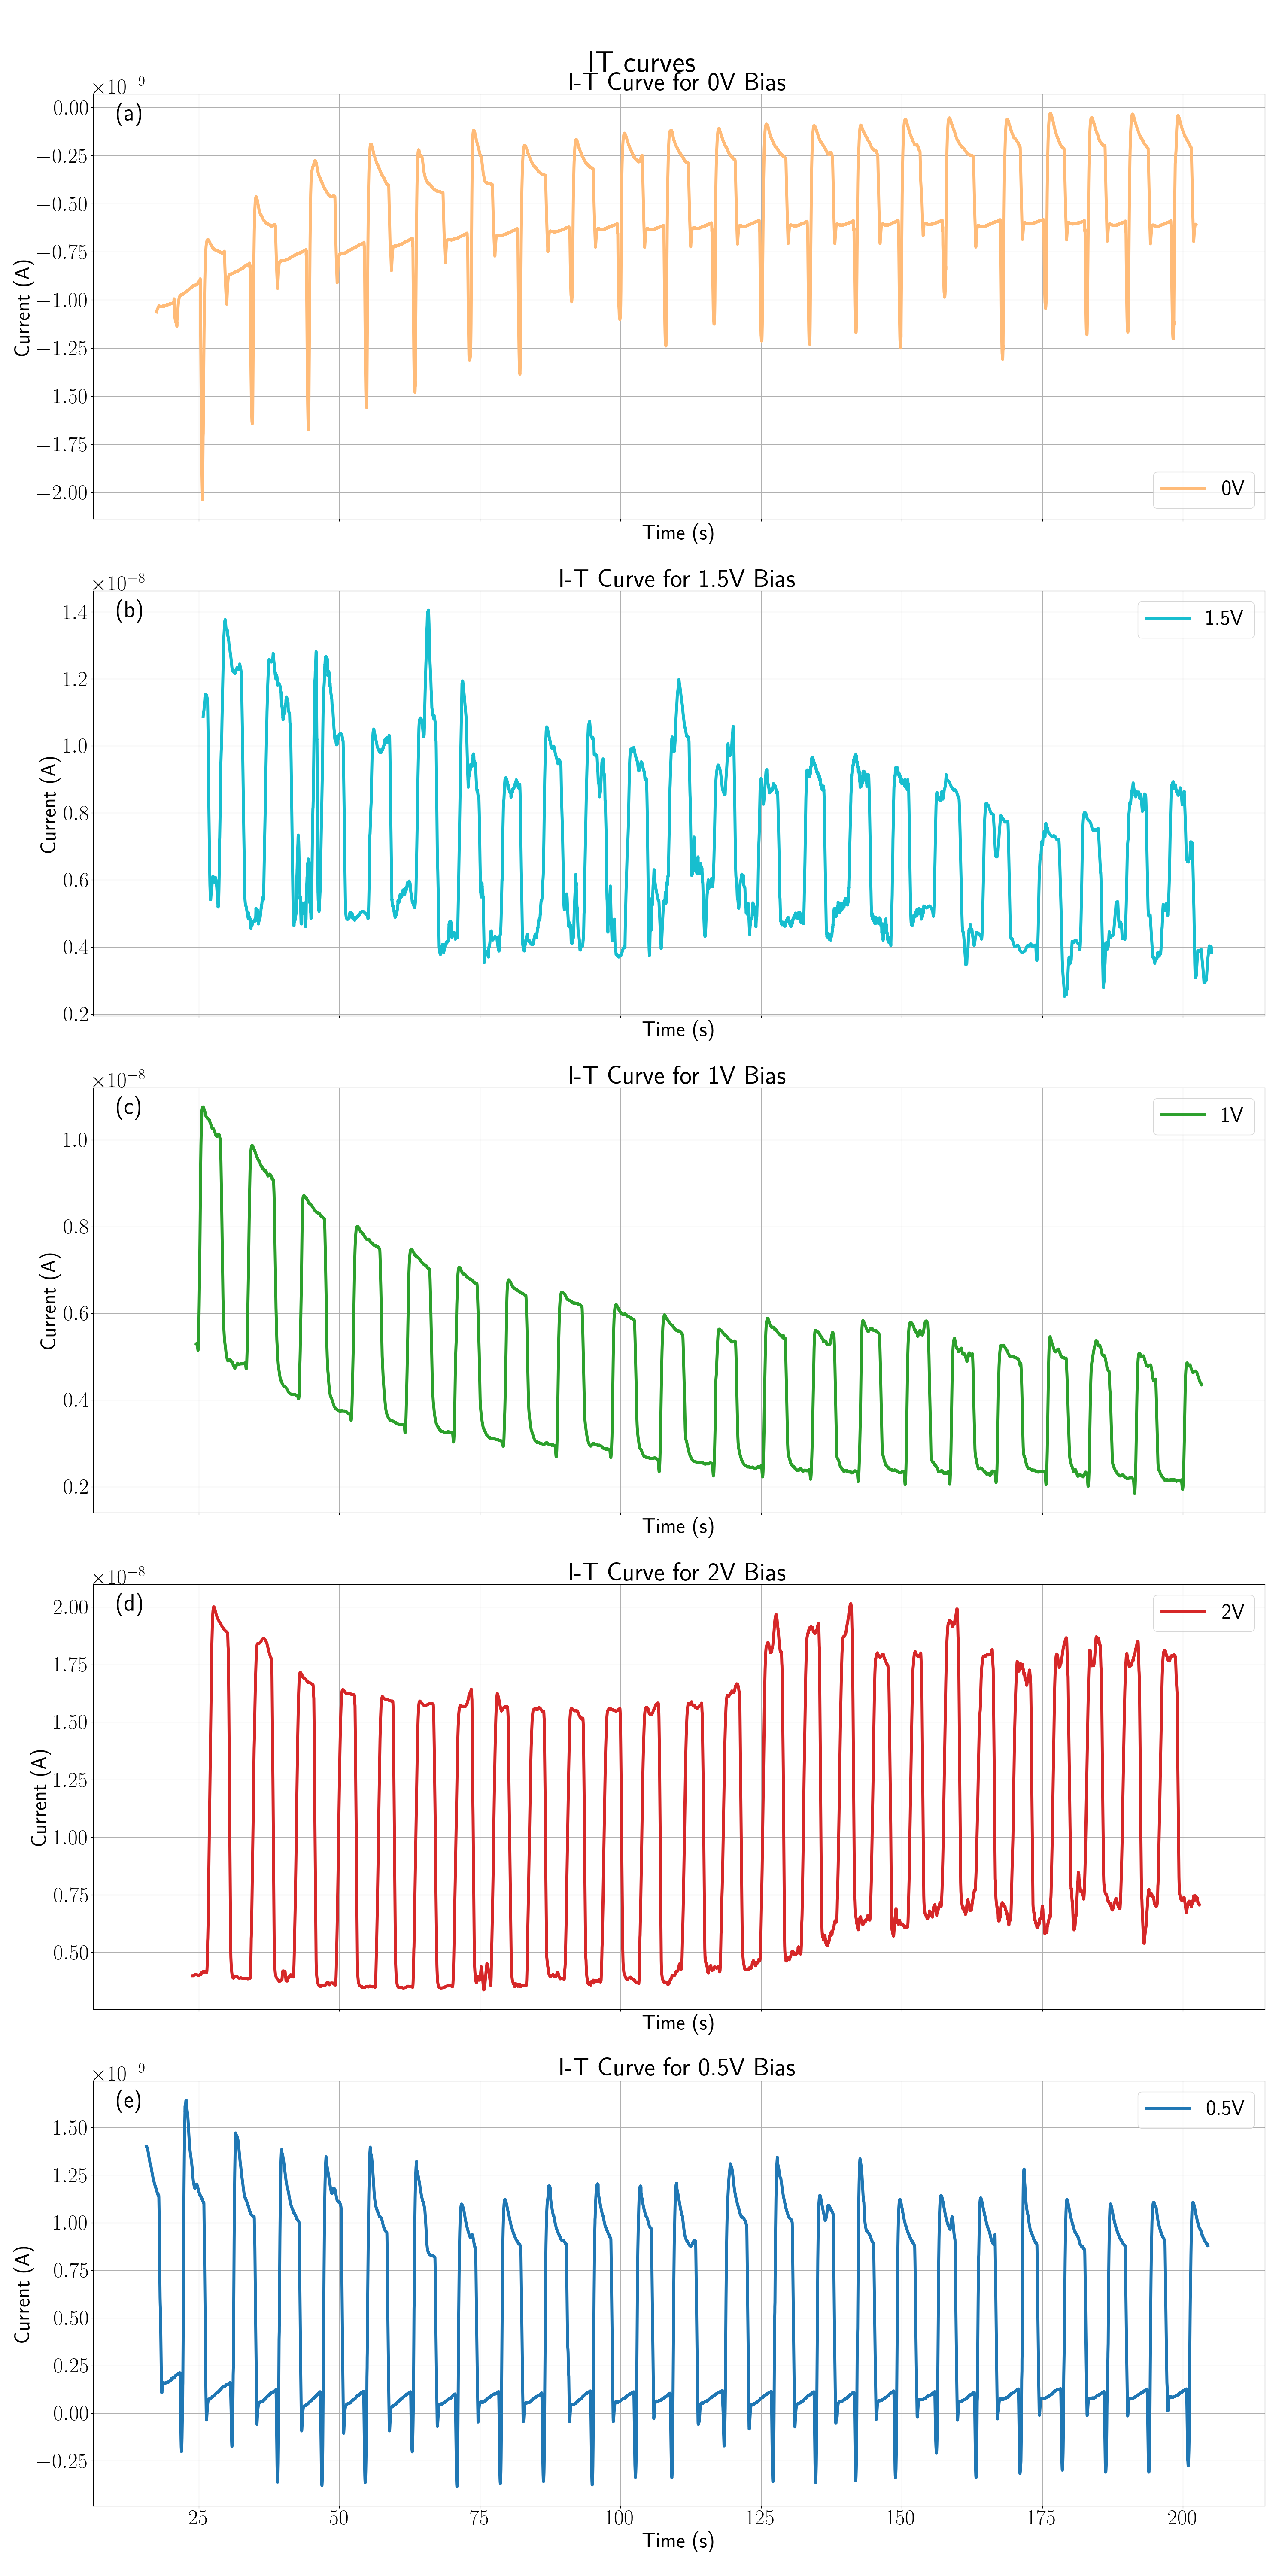
\includegraphics[width=0.7\textwidth]{results/SC/ITs.png}
		\caption{Current Vs. Time curve of the spin coated photo detector }
		\label{fig:IT_individual}
	\end{figure}
	\begin{figure}[htpb]
		\centering
		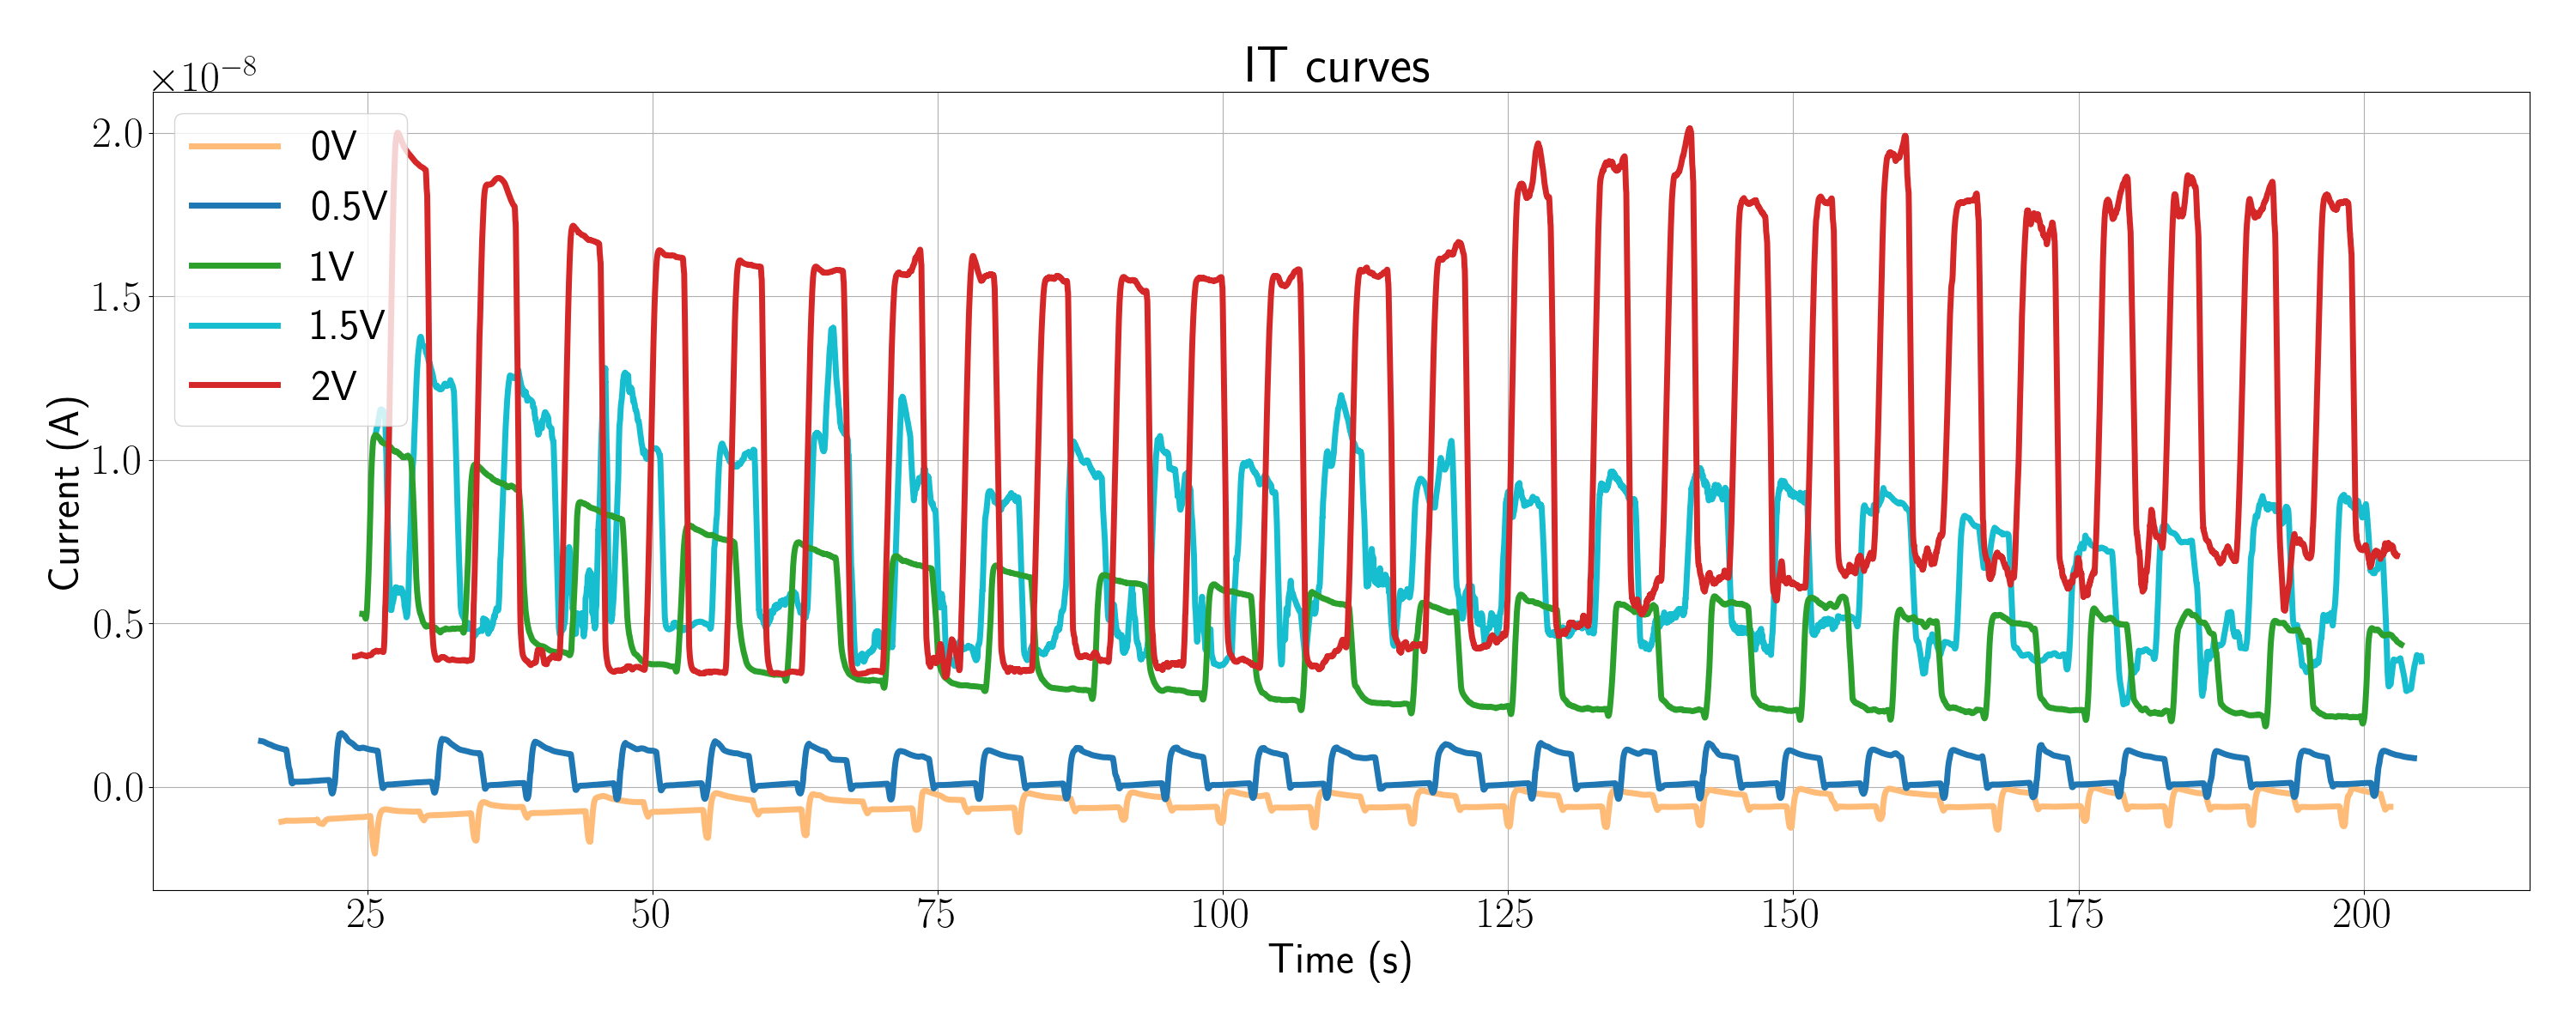
\includegraphics[width=\textwidth]{results/SC/ITs2.png}
		\caption{Overlaid Current Vs. Time curve of the spin coated photo detector}
		\label{fig:IT_combined}
	\end{figure}
		
	
	% Results Section - Electrical Characterization
	

	
	The photoresponse characteristics of the fabricated \ce{MAPbBr3} nanowire photodetectors were investigated through current-time (I - T) measurements under periodic light on/off cycles at various bias voltages. Figure~\ref{fig:IT_individual} presents the temporal photocurrent response at five different bias conditions: $0~V$, $0.5~V$, $1~V$, $1.5~V$, and $2~V$, while Figure~\ref{fig:IT_combined} shows a comparative overlay of all bias conditions.
	
	At zero applied bias, the photodetector exhibited minimal photoresponse, with current oscillations remaining in the picoampere range ($\sim 10^{-9}$~A) as shown in Figure~\ref{fig:IT_individual}(a). The small magnitude of the photocurrent under zero bias conditions indicates weak built-in electric field-driven charge separation at the \ce{ITO}/\ce{MAPbBr3}/Al heterointerfaces. The negative baseline current suggests the presence of a built-in potential, likely arising from the work function difference between the ITO anode and Al cathode, creating a rectifying junction. However, this built-in field alone is insufficient to efficiently separate and collect photogenerated charge carriers, resulting in limited photodetection capability without external bias.
	
	Application of a small forward bias of $0.5~V$ (Figure~\ref{fig:IT_individual}(e)) led to a clear and reproducible photoresponse, with the photocurrent switching between approximately 0 and $1.5 \times 10^{-9}$~A during light on/off cycles. The regular oscillations demonstrate that the device can successfully detect light modulation at this bias level. At 1~V bias (Figure~\ref{fig:IT_individual}(c)), the photoresponse was further enhanced, with photocurrent peaks ranging from approximately $2 \times 10^{-9}$~A to $1.1 \times 10^{-8}$~A. However, a gradual decrease in peak photocurrent intensity over time was observed, indicating the onset of performance degradation during continuous operation.
	
	At $1.5~V$ bias (Figure~\ref{fig:IT_individual}(b)), the device exhibited the strongest initial photoresponse, with photocurrent peaks reaching approximately $1.4 \times 10^{-8}$~A. However, significant degradation was evident throughout the measurement period, with the photocurrent decreasing progressively from the initial peaks of $\sim 1.4 \times 10^{-8}$~A to approximately $8 \times 10^{-9}$~A by the end of the measurement. This substantial decay suggests the accumulation of mobile ions or trapped charges within the perovskite nanowires under prolonged bias and illumination.
	
	Interestingly, at 2~V bias (Figure~\ref{fig:IT_individual}(d)), the device demonstrated the highest absolute photocurrent levels, with peaks reaching approximately $2 \times 10^{-8}$~A. The temporal evolution of the photoresponse at this bias exhibited distinctive behavior: after an initial period of instability and decay during the first $\sim 50$~seconds, the device showed partial recovery and more stable switching characteristics between approximately 125 and 200 seconds. This behavior suggests that the higher electric field may facilitate the redistribution or extraction of accumulated charges, leading to improved stability after an initial ``conditioning'' period.
	
	The overlay of all I - T curves in Figure~\ref{fig:IT_combined} clearly illustrates the bias-dependent photoresponse and the associated stability challenges. The progressive degradation observed at bias voltages above $1~V$ can be attributed to several mechanisms commonly reported in halide perovskite devices:
	
	\begin{enumerate}
		\item \textbf{Ion migration:} Halide perovskites, including \ce{MAPbBr3}, are known to exhibit significant ionic conductivity. Under applied bias and illumination, mobile ions (primarily \ce{Br-} and \ce{MA+}) can migrate through the crystal lattice, leading to the formation of space charge regions and electric field screening. This reduces the effective field available for charge separation and collection.
		
		\item \textbf{Charge trapping:} The one-dimensional nanowire geometry, while beneficial for charge transport along the nanowire axis, may also present a high density of surface trap states due to the large surface-to-volume ratio. Continuous illumination can lead to the progressive filling of these trap states, reducing the density of mobile charge carriers available for photocurrent generation.
		
		\item \textbf{Interface charge accumulation:} Inefficient charge extraction at the \ce{MAPbBr3}/electrode interfaces can result in the accumulation of charges, creating interfacial barriers that oppose further charge injection and extraction.
		
		\item \textbf{Electrochemical reactions:} At higher bias voltages, electrochemical side reactions at the interfaces or within the perovskite material itself may contribute to device degradation.
	\end{enumerate}
	
	The partial recovery observed at $2~V$ after approximately 125 seconds suggests that the higher electric field may help overcome some of these degradation mechanisms, possibly by redistributing accumulated ions or enhancing charge extraction efficiency. Nevertheless, the overall trend indicates that optimizing device stability will require careful engineering of the interfaces, encapsulation strategies, and operational protocols.
	
	\subsubsection{Current-Voltage Characteristics}
	
	\begin{figure}[htpb]
		\centering
		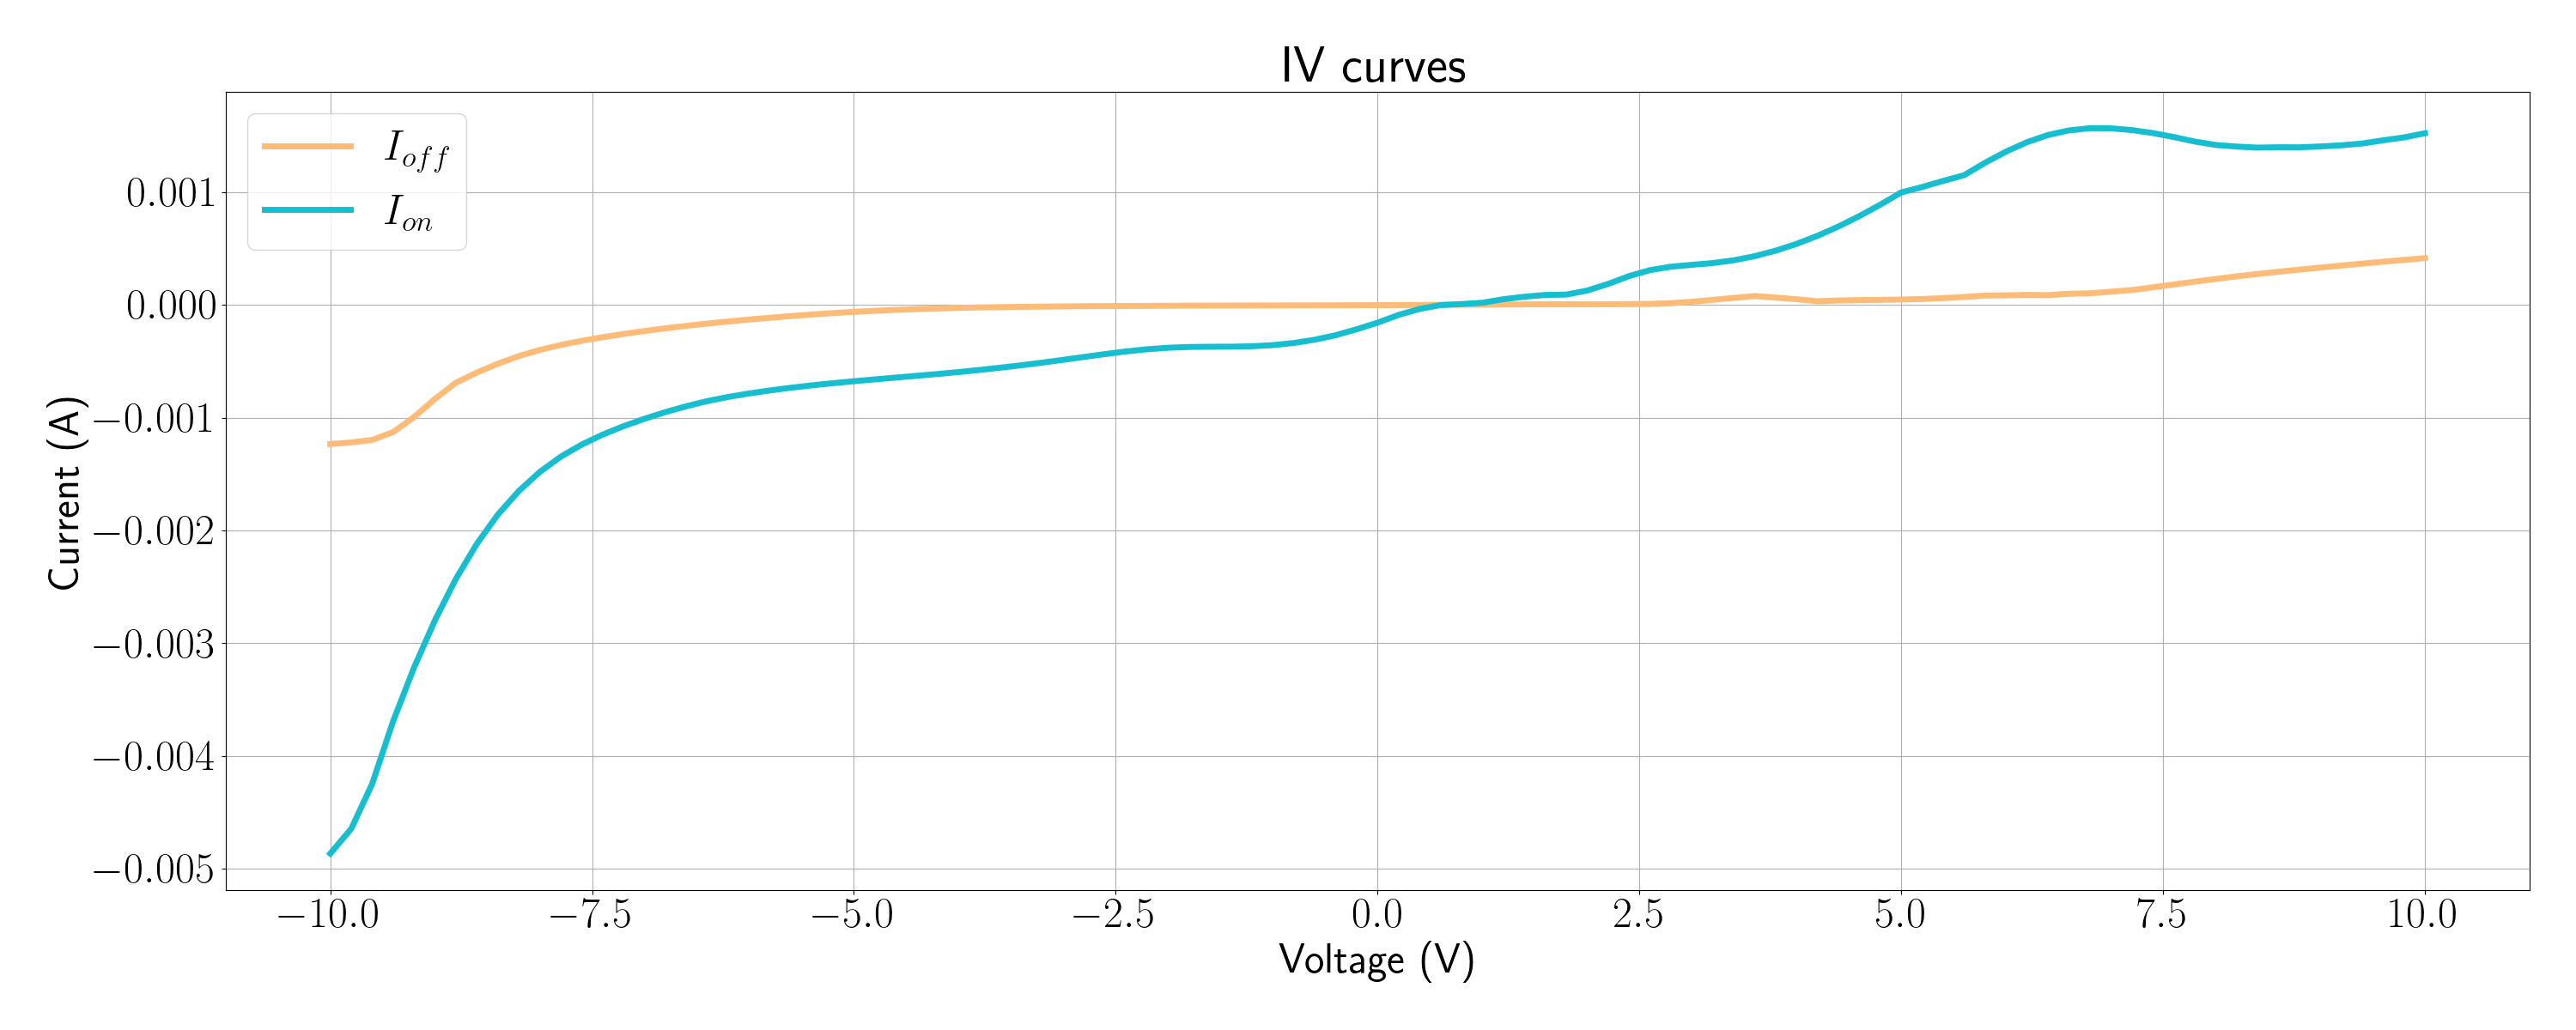
\includegraphics[width=\textwidth]{results/SC/IVs.png}
		\caption{Current Vs. Voltage curve of the spin coated photo detector }
		\label{fig:IV_separate}
	\end{figure}
	\begin{figure}[htpb]
		\centering
		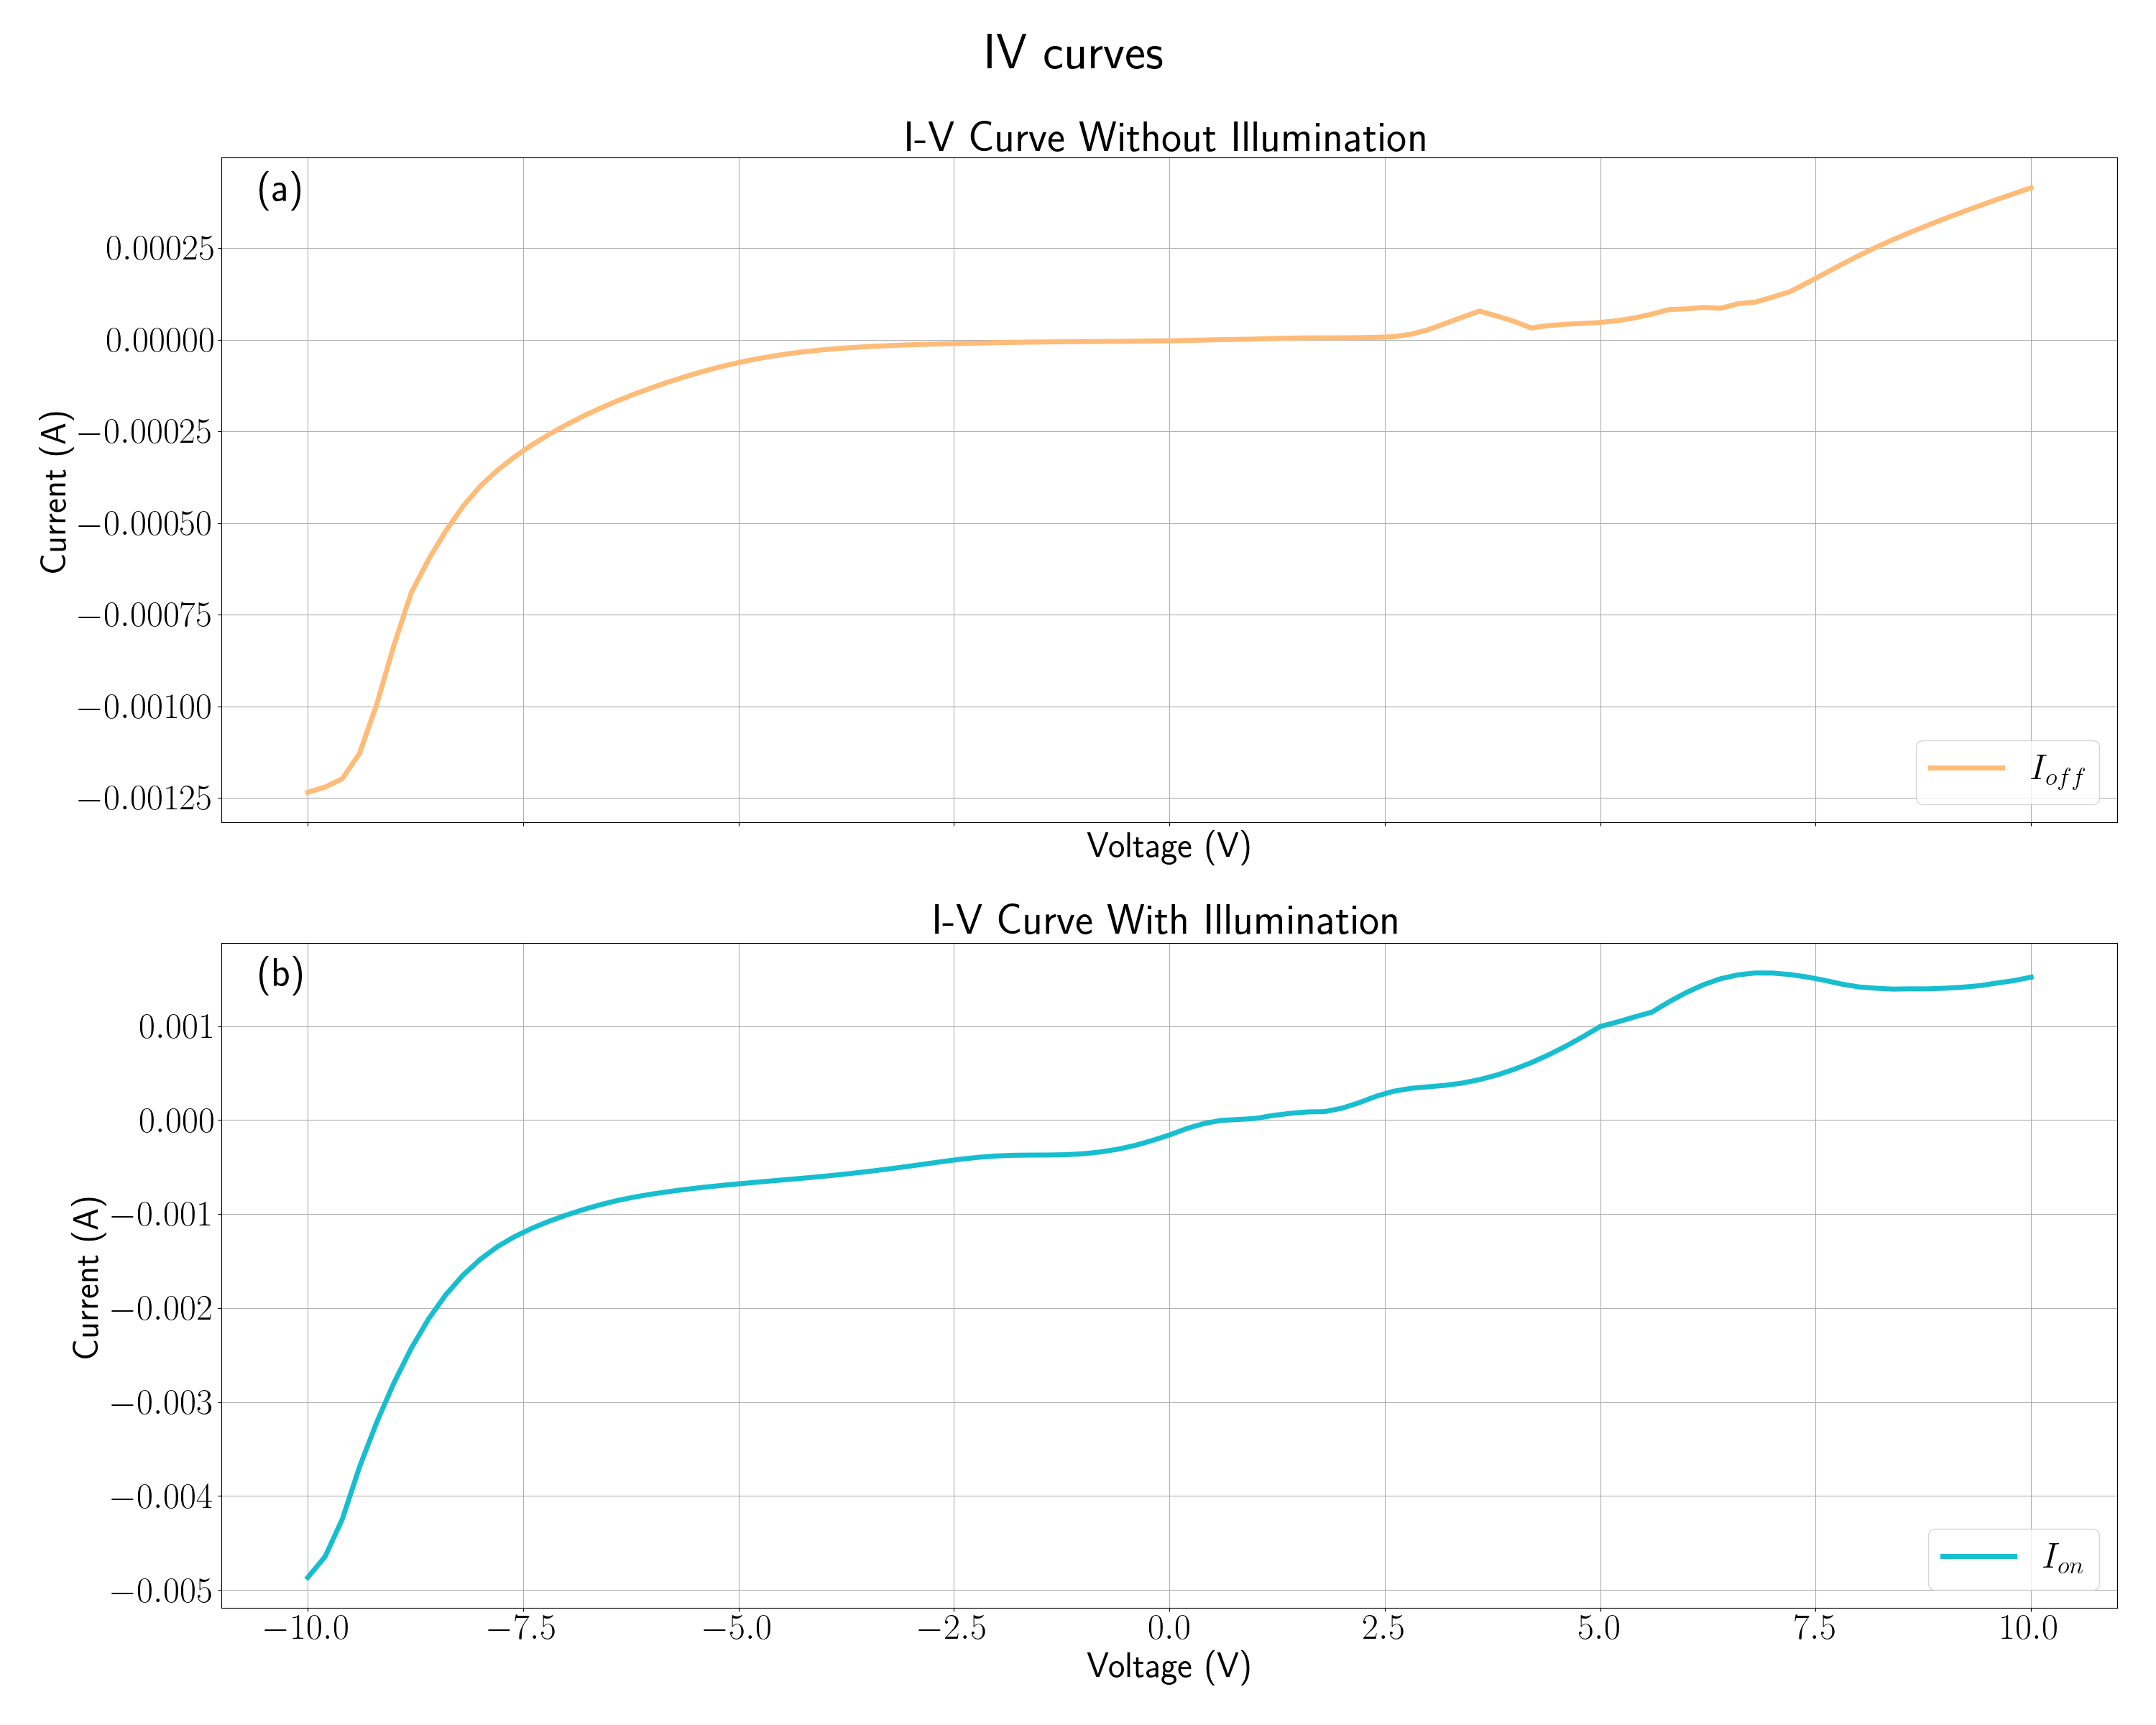
\includegraphics[width=\textwidth]{results/SC/IVs2.png}
		\caption{Overlaid Current Vs. Voltage curve of the spin coated photo detector}
		\label{fig:IV_overlay}
	\end{figure}
		
	The current-voltage (I - V) characteristics of the photodetector were measured in both dark and illuminated conditions to evaluate the rectification behavior and photoresponsive properties of the device. Figure~\ref{fig:IV_separate} presents the separate I - V curves for dark ($I_{\text{off}}$) and illuminated ($I_{\text{on}}$) conditions, while Figure~\ref{fig:IV_overlay} shows both curves overlaid for direct comparison.
	
	The dark current curve (Figure~\ref{fig:IV_separate}(a)) exhibits clear rectifying behavior, characteristic of a Schottky or heterojunction diode. Under reverse bias (negative voltages), the dark current is suppressed to approximately $-1.25 \times 10^{-3}$~A at $-10$~V, indicating relatively low leakage current. This suggests the formation of an effective energy barrier at one or both of the \ce{ITO}/\ce{MAPbBr3} and \ce{MAPbBr3}/Al interfaces.
	
	In the forward bias regime (positive voltages), the dark current increases exponentially at low voltages, consistent with thermionic emission over the Schottky barrier. At higher positive voltages (above $\sim 5$~V), the current continues to increase but with a reduced slope, reaching approximately $4 \times 10^{-4}$~A at $+10$~V. This behavior suggests the presence of series resistance, which becomes significant at higher current levels, and may arise from the resistivity of the nanowire array, contact resistance at the electrodes, or the resistance of the PAA template itself.
	
	Under illumination (Figure~\ref{fig:IV_separate}(b)), the I - V curve shows a substantial increase in current across the entire voltage range, clearly demonstrating the photoresponsive nature of the device. The photocurrent reaches approximately $-5 \times 10^{-3}$~A at $-10$~V and approximately $1.5 \times 10^{-3}$~A at $+10$~V, representing a significant enhancement compared to the dark current.
	
	The overlay plot (Figure~\ref{fig:IV_overlay}) emphasizes the strong light-to-dark current ratio, particularly in the reverse bias regime, where the photocurrent enhancement is most pronounced. This indicates efficient photogeneration and collection of charge carriers when the device is operated under reverse bias, where the built-in electric field is reinforced by the external bias.
	
	The asymmetric I - V characteristics, with higher current magnitudes under reverse bias compared to forward bias (under illumination), are noteworthy. This behavior differs from typical photodiode operation and suggests that:
	
	\begin{enumerate}
		\item The device architecture creates a preferential direction for charge collection, possibly due to asymmetric energy band alignment at the ITO and Al contacts.
		\item The nanowire/template configuration may introduce additional rectification mechanisms beyond simple metal-semiconductor contacts.
		\item Interface states or dipoles at the electrode interfaces may modify the effective barrier heights for electron and hole injection/extraction.
	\end{enumerate}
	
	An important observation in the photocurrent curve is the apparent saturation or slight decrease at high positive bias voltages (above $\sim 6$~V). This behavior could be attributed to several factors:
	
	\begin{enumerate}
		\item \textbf{Charge recombination:} At very high electric fields, the increased carrier density may enhance bimolecular or Auger recombination rates, offsetting the gains from improved charge extraction.
		\item \textbf{Contact limitations:} The finite charge injection/extraction rate at the electrode interfaces may limit the current, leading to saturation despite increased bias.
		\item \textbf{Joule heating:} High current flow may cause localized heating, which can reduce carrier mobility and increase recombination rates in the perovskite nanowires.
		\item \textbf{Space charge effects:} At high bias, space charge accumulation near the electrodes may screen the applied electric field within the active nanowire region.
	\end{enumerate}
	
	\subsubsection{Photodetector Performance Metrics}
	
	To quantitatively assess the performance of the fabricated \ce{MAPbBr3} nanowire photodetector, three key figures of merit were calculated: photocurrent ($I_{\text{ph}}$), responsivity ($R$), and specific detectivity ($D^{\ast}$). These parameters were evaluated as functions of both light intensity (Figure~\ref{fig:metrics_intensity}) and applied bias voltage (Figure~\ref{fig:metrics_voltage}).
	
	
	
	\begin{figure}[htpb]
		\centering
		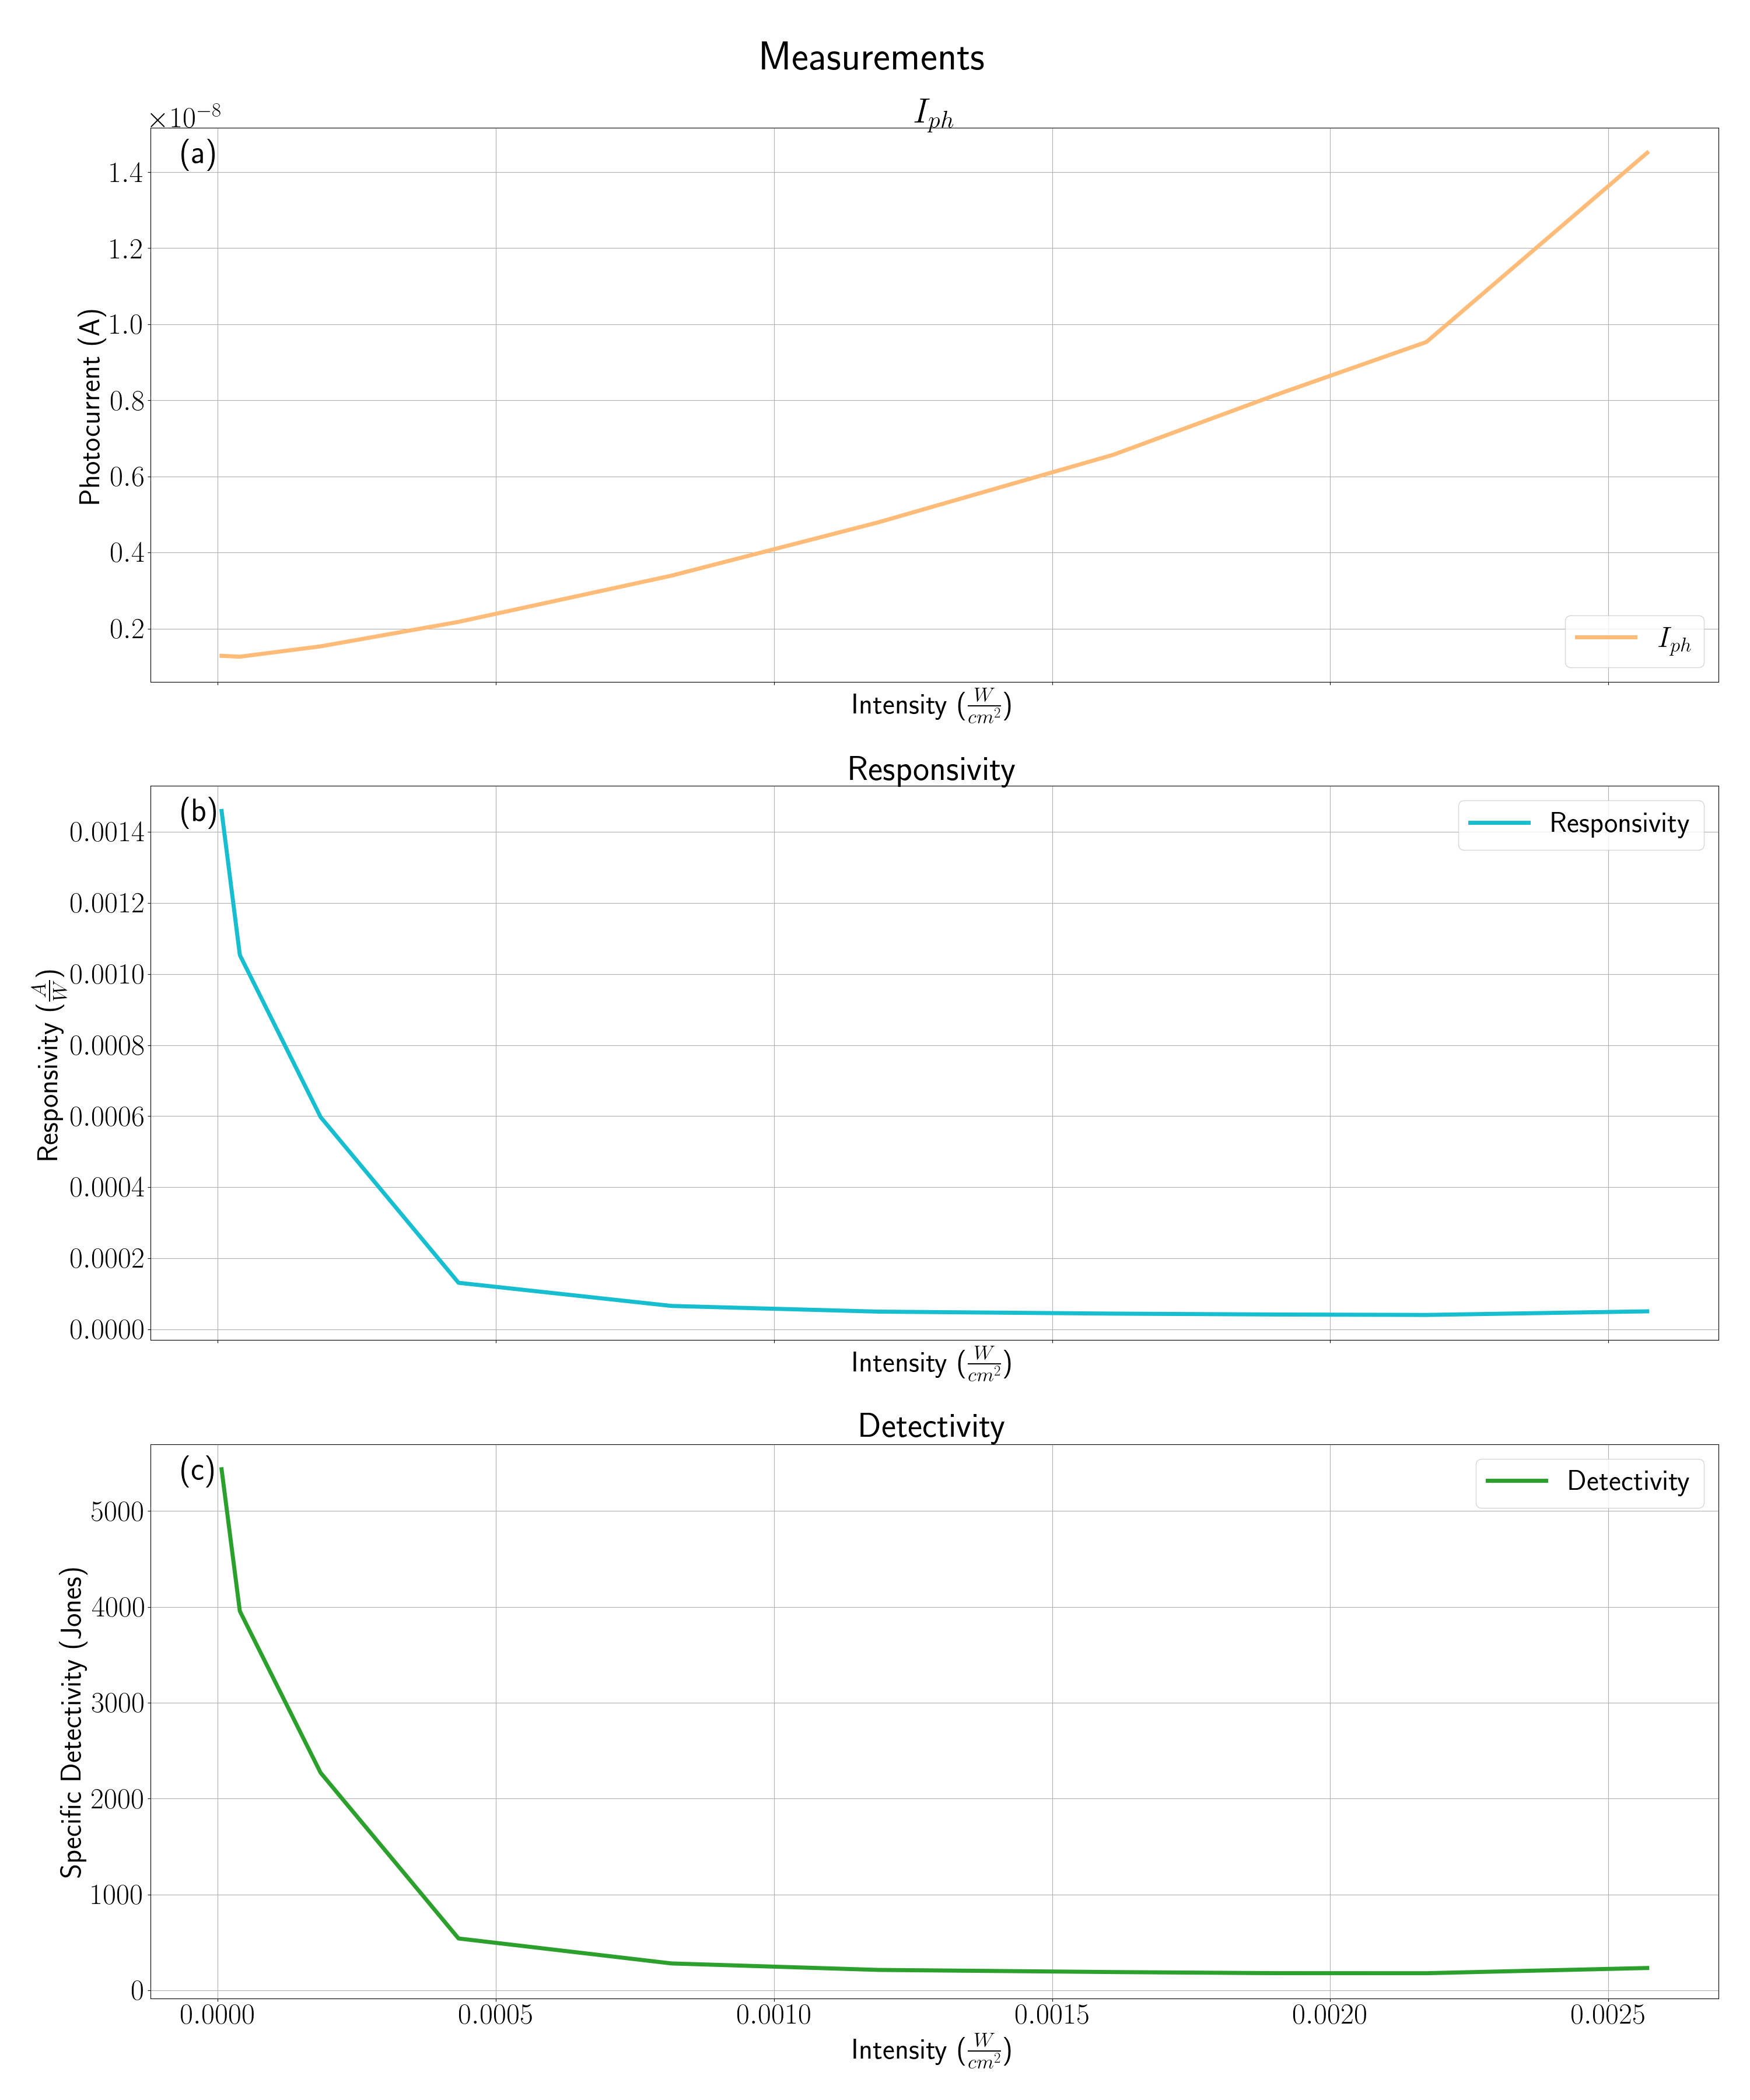
\includegraphics[width=\textwidth]{results/SC/meas.png}
		\caption{Photo Detector measurements Vs. light intensity}
		\label{fig:metrics_intensity}
	\end{figure}

	\begin{figure}[htpb]
		\centering
		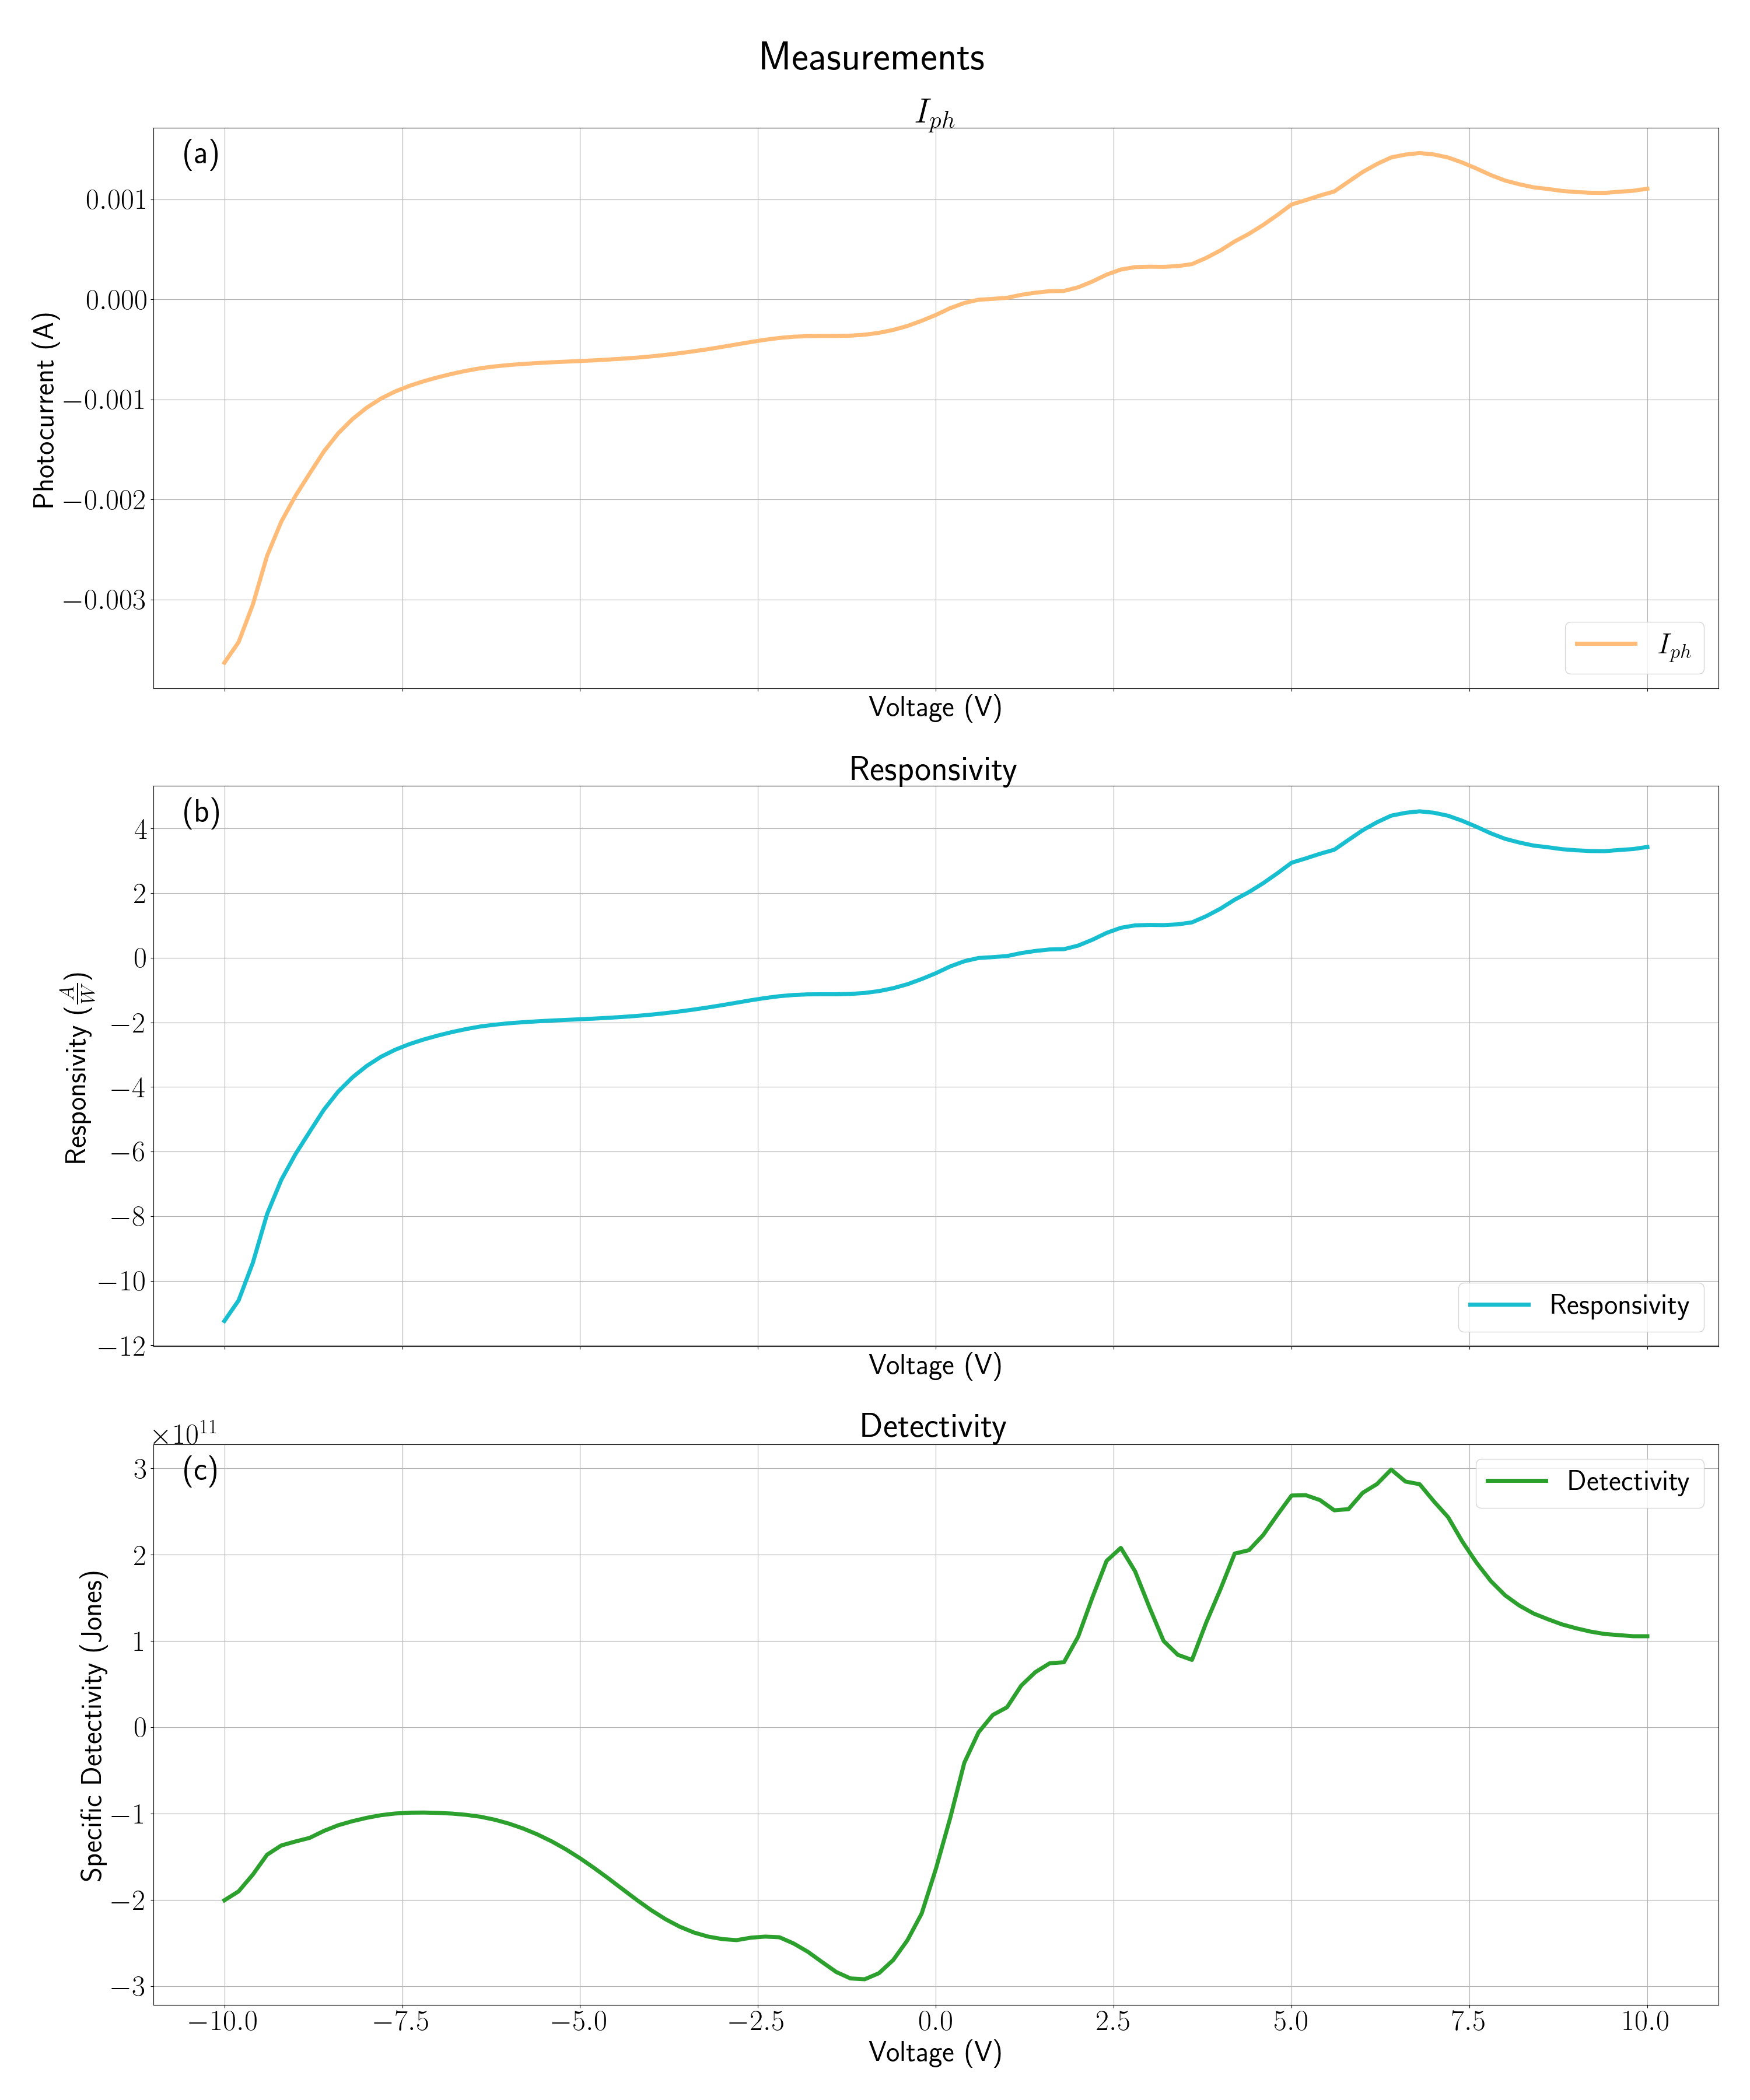
\includegraphics[width=\textwidth]{results/SC/measurements.png}
		\caption{Photo Detector measurements Vs. bias voltage}
		\label{fig:metrics_voltage}
	\end{figure}
	
	The photocurrent, defined as the difference between the illuminated and dark currents ($I_{\text{ph}} = I_{\text{on}} - I_{\text{off}}$), represents the net current generated by photoexcited carriers. 
	
	Based on Figure~\ref{fig:metrics_intensity}(a), the photocurrent increases monotonically with light intensity, as expected, but exhibits a sublinear relationship. At the lowest measured intensity, $I_{\text{ph}} \approx 1 \times 10^{-9}$~A, increasing to approximately $1.4 \times 10^{-8}$~A at the highest intensity. The sublinear behavior, where the photocurrent increases at a rate slower than the incident light intensity, is characteristic of photodetectors with significant trap-mediated recombination. As the light intensity increases, trap states become progressively saturated, and the relative contribution of recombination losses increases, resulting in reduced photoconversion efficiency at higher intensities.
	
	Based on Figure~\ref{fig:metrics_voltage}(a)), the photocurrent shows strong voltage dependence, with a sharp transition from negative to positive values around $0~V$, consistent with the rectifying nature of the device. The photocurrent magnitude increases with increasing positive bias, reaching a maximum of approximately $1.1 \times 10^{-3}$~A at high positive voltages ($\sim 7$~V), before showing signs of saturation. This voltage-dependent behavior confirms that external bias is essential for efficient charge extraction in this device architecture.
	
	Responsivity ($R$) quantifies the photocurrent generated per unit incident optical power and is calculated as:
	\begin{equation}
		R = \frac{I_{\text{ph}}}{P_{\text{in}}} = \frac{I_{\text{ph}}}{A \cdot I_{\text{light}}}
	\end{equation}
	where $P_{\text{in}}$ is the incident optical power, $A$ is the active device area, and $I_{\text{light}}$ is the incident light intensity.

	Based on Figure~\ref{fig:metrics_intensity}(b)), the responsivity exhibits a dramatic intensity-dependent behavior. At the lowest measured light intensity, the responsivity reaches an exceptionally high value of approximately $1.5 \times 10^{-3}$~A/W, indicating excellent sensitivity in the low-light regime. However, as the intensity increases, the responsivity decreases sharply, falling below $2 \times 10^{-4}$~A/W at moderate intensities and stabilizing at even lower values ($\sim 5 \times 10^{-5}$~A/W) at the highest intensities.
	
	This strong intensity dependence of responsivity is directly related to the sublinear photocurrent-intensity relationship discussed above. The high responsivity at low intensities suggests that the device is optimized for low-light detection applications, where trap-assisted photocurrent gain mechanisms may enhance the effective quantum efficiency. However, the rapid decrease with increasing intensity limits the dynamic range of the detector.
	
	
	Based on Figure~\ref{fig:metrics_voltage}(b)), the responsivity shows significant voltage dependence, with negative values at negative bias (indicating unfavorable operation under reverse bias for this particular configuration) and a sharp increase in the positive bias regime. The responsivity reaches a maximum of approximately $4 - 5~A/W$ at moderate positive bias (around $5 - 7~V$), demonstrating that the device achieves optimal photoconversion efficiency in this voltage range. The subsequent slight decrease at higher voltages correlates with the photocurrent saturation behavior observed in the I - V characteristics.
	
	Specific detectivity ($D^{\ast}$) is a normalized figure of merit that accounts for both the responsivity and the noise characteristics of the detector, defined as:
	\begin{equation}
		D^* = \frac{R \sqrt{A}}{i_n} = \frac{R \sqrt{A}}{\sqrt{2eI_{\text{dark}}}}
	\end{equation}
	where $i_n$ is the noise current, approximated here by shot noise from the dark current ($i_n = \sqrt{2eI_{\text{dark}}}$), $e$ is the elementary charge, and $A$ is the active device area. $D^*$ is typically expressed in Jones (cm·Hz$^{1/2}$·W$^{-1}$).
	
	Based on Figure~\ref{fig:metrics_intensity}(c), the detectivity shows a similar trend to responsivity, with exceptionally high values at low light intensities. At the lowest intensity, $D^*$ reaches approximately $5 \times 10^3$~Jones, indicating excellent capability for detecting weak optical signals. As the intensity increases, the detectivity decreases rapidly, stabilizing at approximately $200 - 300~Jones$ at higher intensities. This behavior is typical for photodetectors limited by trap states and recombination losses, where the signal-to-noise ratio degrades at higher illumination levels.
	
	Basec on Figure~\ref{fig:metrics_voltage}(c), the detectivity as a function of voltage reveals the most favorable operating regime for the photodetector. At negative bias voltages, the detectivity shows negative values, indicating that the device does not operate efficiently in this regime. Around zero bias, complex oscillatory behavior is observed, likely related to the transition between rectification regimes and the competing effects of built-in field and external bias.
	
	At positive bias, the detectivity increases sharply, reaching a maximum of approximately $3 \times 10^{11}$~Jones at moderate positive voltages ($5 - 7~V$). This exceptionally high detectivity demonstrates that the device can achieve excellent sensitivity when operated at the optimal bias point. The subsequent decrease at higher voltages correlates with increased dark current and the onset of photocurrent saturation effects.
	
	\subsubsection{Discussion and Performance Comparison}
	
	The electrical characterization results demonstrate that the \ce{MAPbBr3} nanowire photodetectors fabricated via the spin-coating method exhibit clear photoresponsive behavior with bias-tunable performance. The key findings and their implications are discussed below.
	
	\paragraph{Photoresponse and Stability}
	
	The I - T measurements reveal that while the device shows good switching behavior and reproducible photoresponse, stability remains a critical challenge, particularly at higher bias voltages. The observed degradation mechanisms—likely involving ion migration, charge trapping, and interfacial charge accumulation—are characteristic of halide perovskite devices and have been widely reported in the literature. The partial recovery at$ 2~V$ bias after initial degradation suggests that operation under pulsed bias or intermittent illumination protocols may improve long-term stability.
	
	Future work should focus on:
	\begin{itemize}
		\item Implementing effective encapsulation strategies to minimize environmental degradation
		\item Engineering the electrode interfaces to reduce ion migration and improve charge extraction efficiency
		\item Exploring interfacial buffer layers to passivate trap states
		\item Developing operational protocols that minimize continuous high-bias operation
	\end{itemize}
	
	\paragraph{Current-Voltage Characteristics and Device Physics}
	
	The rectifying I - V characteristics confirm the formation of effective charge-selective contacts in the \ce{ITO}/\ce{MAPbBr3}/Al heterostructure. The strong photoresponse across a broad voltage range validates the functionality of the vertically aligned nanowire architecture for photodetection. However, the asymmetric behavior and the observation of higher photocurrent magnitudes under reverse bias warrant further investigation of the energy band alignment and charge transport mechanisms at the nanowire/electrode interfaces.
	
	The photocurrent saturation at high forward bias suggests that device performance is ultimately limited by factors beyond simple electric field enhancement, such as contact resistance, heat dissipation, or intrinsic recombination processes. Optimization of the contact materials and interface engineering could potentially extend the linear operation range and improve high-power performance.
	
	\paragraph{Performance Metrics and Operating Regime}
	
	The comprehensive analysis of photocurrent, responsivity, and detectivity as functions of both intensity and voltage provides valuable insights into the optimal operating conditions for the fabricated photodetectors:
	
	\begin{itemize}
		\item \textbf{Low-light detection:} The device exhibits exceptional sensitivity at low light intensities, with detectivity values reaching $\sim 10^{11}$~Jones. This makes it particularly suitable for applications requiring detection of weak optical signals, such as environmental sensing or low-light imaging.
		
		\item \textbf{Optimal bias point:} Operation at moderate positive bias ($5 - 7~V$) provides the best balance between responsivity, detectivity, and stability. At this operating point, the device achieves responsivity of $4 - 5~A/W$ and detectivity exceeding $10^{11}$~Jones.
		
		\item \textbf{Limited dynamic range:} The strong intensity dependence of responsivity and detectivity, with rapid degradation at higher light intensities, indicates a limited linear dynamic range. This is a trade-off inherent to high-sensitivity photodetectors with gain mechanisms and represents an area for future optimization.
		
		\item \textbf{Trade-off between sensitivity and linearity:} The device design prioritizes sensitivity over linearity, which is appropriate for specific applications but may limit its use in applications requiring accurate measurement of wide-ranging light intensities.
	\end{itemize}
	
	In conclusion, the electrical characterization demonstrates that the spin-coated \ce{MAPbBr3} nanowire photodetectors exhibit promising performance characteristics, particularly for low-light detection applications. While stability and linearity remain challenges, the high detectivity and clear photoresponse validate the template-assisted fabrication approach and provide a foundation for further optimization and device engineering.
	
	
	
	\subsection{Characterization of CVD-Grown MAPbI3 Nanowire Photodetectors}
	
	The CVD-grown \ce{MAPbI3} nanowires were characterized using scanning electron microscopy (SEM) to assess their morphology, followed by electrical and optoelectronic measurements to evaluate their performance as photodetectors.
	
	\subsubsection{Morphology}
	
	SEM micrographs reveal vertically aligned \ce{MAPbI3} nanowires confined within the porous anodic alumina (PAA) template channels. The nanowires exhibit lengths ranging from approximately $2.46 \mu m$ to $4.00 \mu m$, with an average of $3.4 \mu m$, as shown in the cross-sectional view (Figure~\ref{fig:cvdsem1}). High-magnification top-view images display densely packed nanowire arrays with circular cross-sections and diameters estimated at $200 - 300 nm$, consistent with the PAA pore dimensions (Figure~\ref{fig:cvdsem2} and \ref{fig:cvdsem3}). The array density is approximately $4 \times 10^{8}$ to $10^{9}$ cm$^{-2}$, indicating high filling efficiency. Side-view SEM confirms uniform vertical alignment with minimal defects or bundling (Figure~\ref{fig:cvdsem4}), suggestive of high crystallinity achieved through the vapor-phase confined growth process.
	
	
	
		\begin{figure}[htpb]
		\centering
		% Panel (a)
		\begin{subfigure}[b]{0.45\textwidth}
			\centering
			\includegraphics[width=\textwidth,]{imgs/TVCVD.jpg}
			\caption{Top view SEM image of the CVD photo detector}
			\label{fig:cvdsem2}
		\end{subfigure}
		\hfill
		% Panel (b)
		\begin{subfigure}[b]{0.45\textwidth}
			\centering
			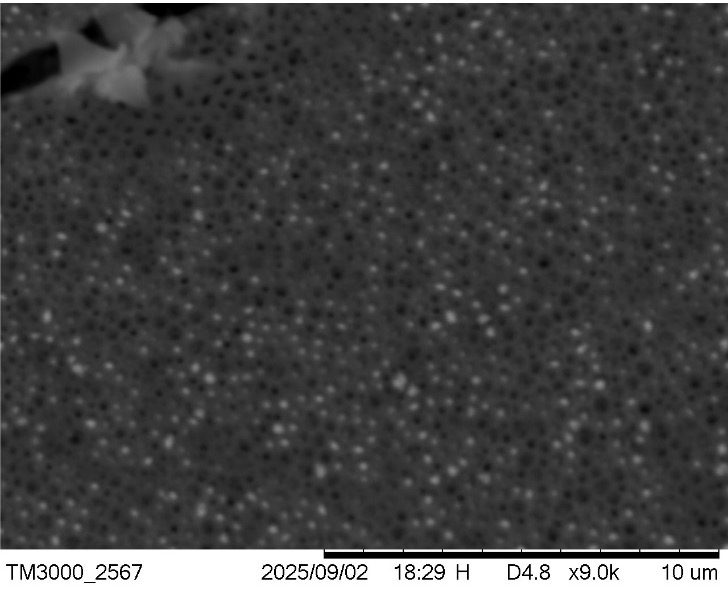
\includegraphics[width=\textwidth]{imgs/TVCVD2.jpg}
			\caption{Another top view SEM image of the CVD photo detector}
			\label{fig:cvdsem3}
		\end{subfigure}
		
		\vspace{0.3cm} % optional spacing between rows
		
		% Panel (c)
		\begin{subfigure}[b]{0.45\textwidth}
			\centering
			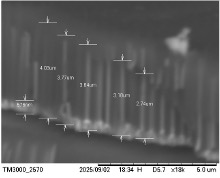
\includegraphics[width=\textwidth]{imgs/CVCVD.jpg}
			\caption{Cross section view SEM image of the CVD photo detector}
			\label{fig:cvdsem1}
		\end{subfigure}
		\hfill
		%panel (d)
		\begin{subfigure}[b]{0.45\textwidth}
			\centering
			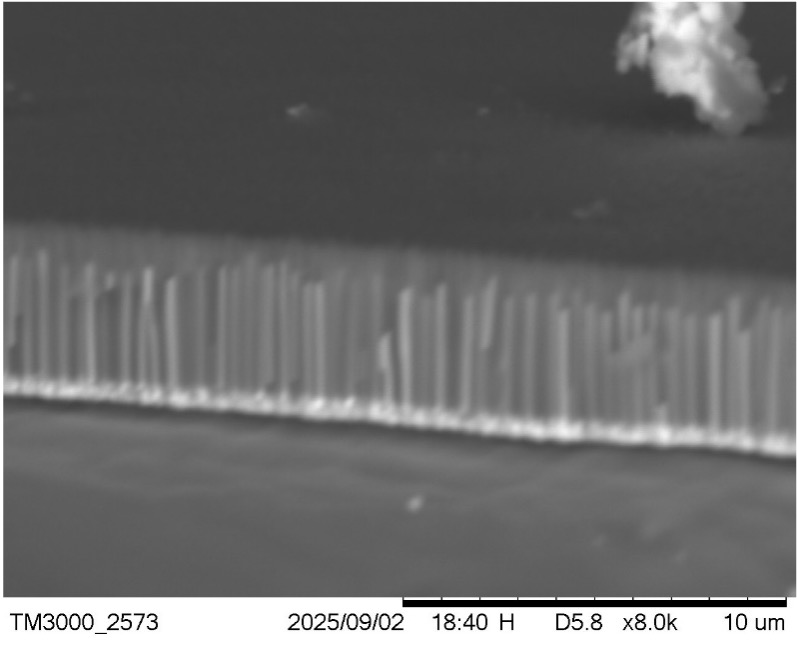
\includegraphics[width=\textwidth]{imgs/CVCVD2.jpg}
			\caption{Another cross section view SEM image of the CVD photo detector}
			\label{fig:cvdsem4}
		\end{subfigure}
		
		\caption{SEM images of the CVD photo detector}
		\label{fig:CVDSEM}
	\end{figure}
	
	
	\subsubsection{Electrical and Optoelectronic Properties}
	
	Current - voltage ($I$ - $V$) characteristics were measured in the dark and under illumination to evaluate the photodetection capabilities. In the dark, the device exhibits a low current ($I_{off}$) on the order of $-4 \times 10^{-6}$ A at $-1$ V, with rectifying behavior indicating Schottky-like contacts (Figure~\ref{fig:CVDIV_separate}(a)). Under white light illumination , the current ($I_{on}$) increases significantly to approximately $-1.4 \times 10^{-5}$ A at $-1$ V, yielding an on/off ratio exceeding 3 (Figure~\ref{fig:CVDIV_separate}(b)). The overlaid $I$ - $V$ curves highlight the photoresponse, with enhanced conductivity under light due to photogenerated carriers (Figure~\ref{fig:CVDIV_overlay}).
	
	
	\begin{figure}[htpb]
		\centering
		\includegraphics[width=\textwidth]{results/CVD/IVs2.png}
		\caption{Current Vs. Voltage curve of the CVD photo detector }
		\label{fig:CVDIV_separate}
	\end{figure}
	\begin{figure}[htpb]
		\centering
		\includegraphics[width=\textwidth]{results/CVD/IVs.png}
		\caption{Overlaid Current Vs. Voltage curve of the CVD photo detector}
		\label{fig:CVDIV_overlay}
	\end{figure}
	
	
	Time-dependent current ($I$ - $T$) measurements under periodic illumination demonstrate stable switching behavior at various biases. At $-0.5$ V bias, the current switches between approximately $-5 \times 10^{-9}$ A (dark) and higher values under light, showing fast response times (Figure~\ref{fig:CVDIT_individual}(a)). At $0$ V (self-powered mode), the photocurrent reaches peaks of $1.4 \times 10^{-8}$ A (Figure~\ref{fig:CVDIT_individual}(b)). At $1$ V, the current exhibits higher magnitudes up to $2 \times 10^{-8}$ A, with consistent on/off cycling over $200$ s (Figure~\ref{fig:CVDIT_individual}(c)). The response and recovery times are estimated to be on the order of milliseconds, based on the sharp transitions.
	
		
	\begin{figure}[htpb]
		\centering
		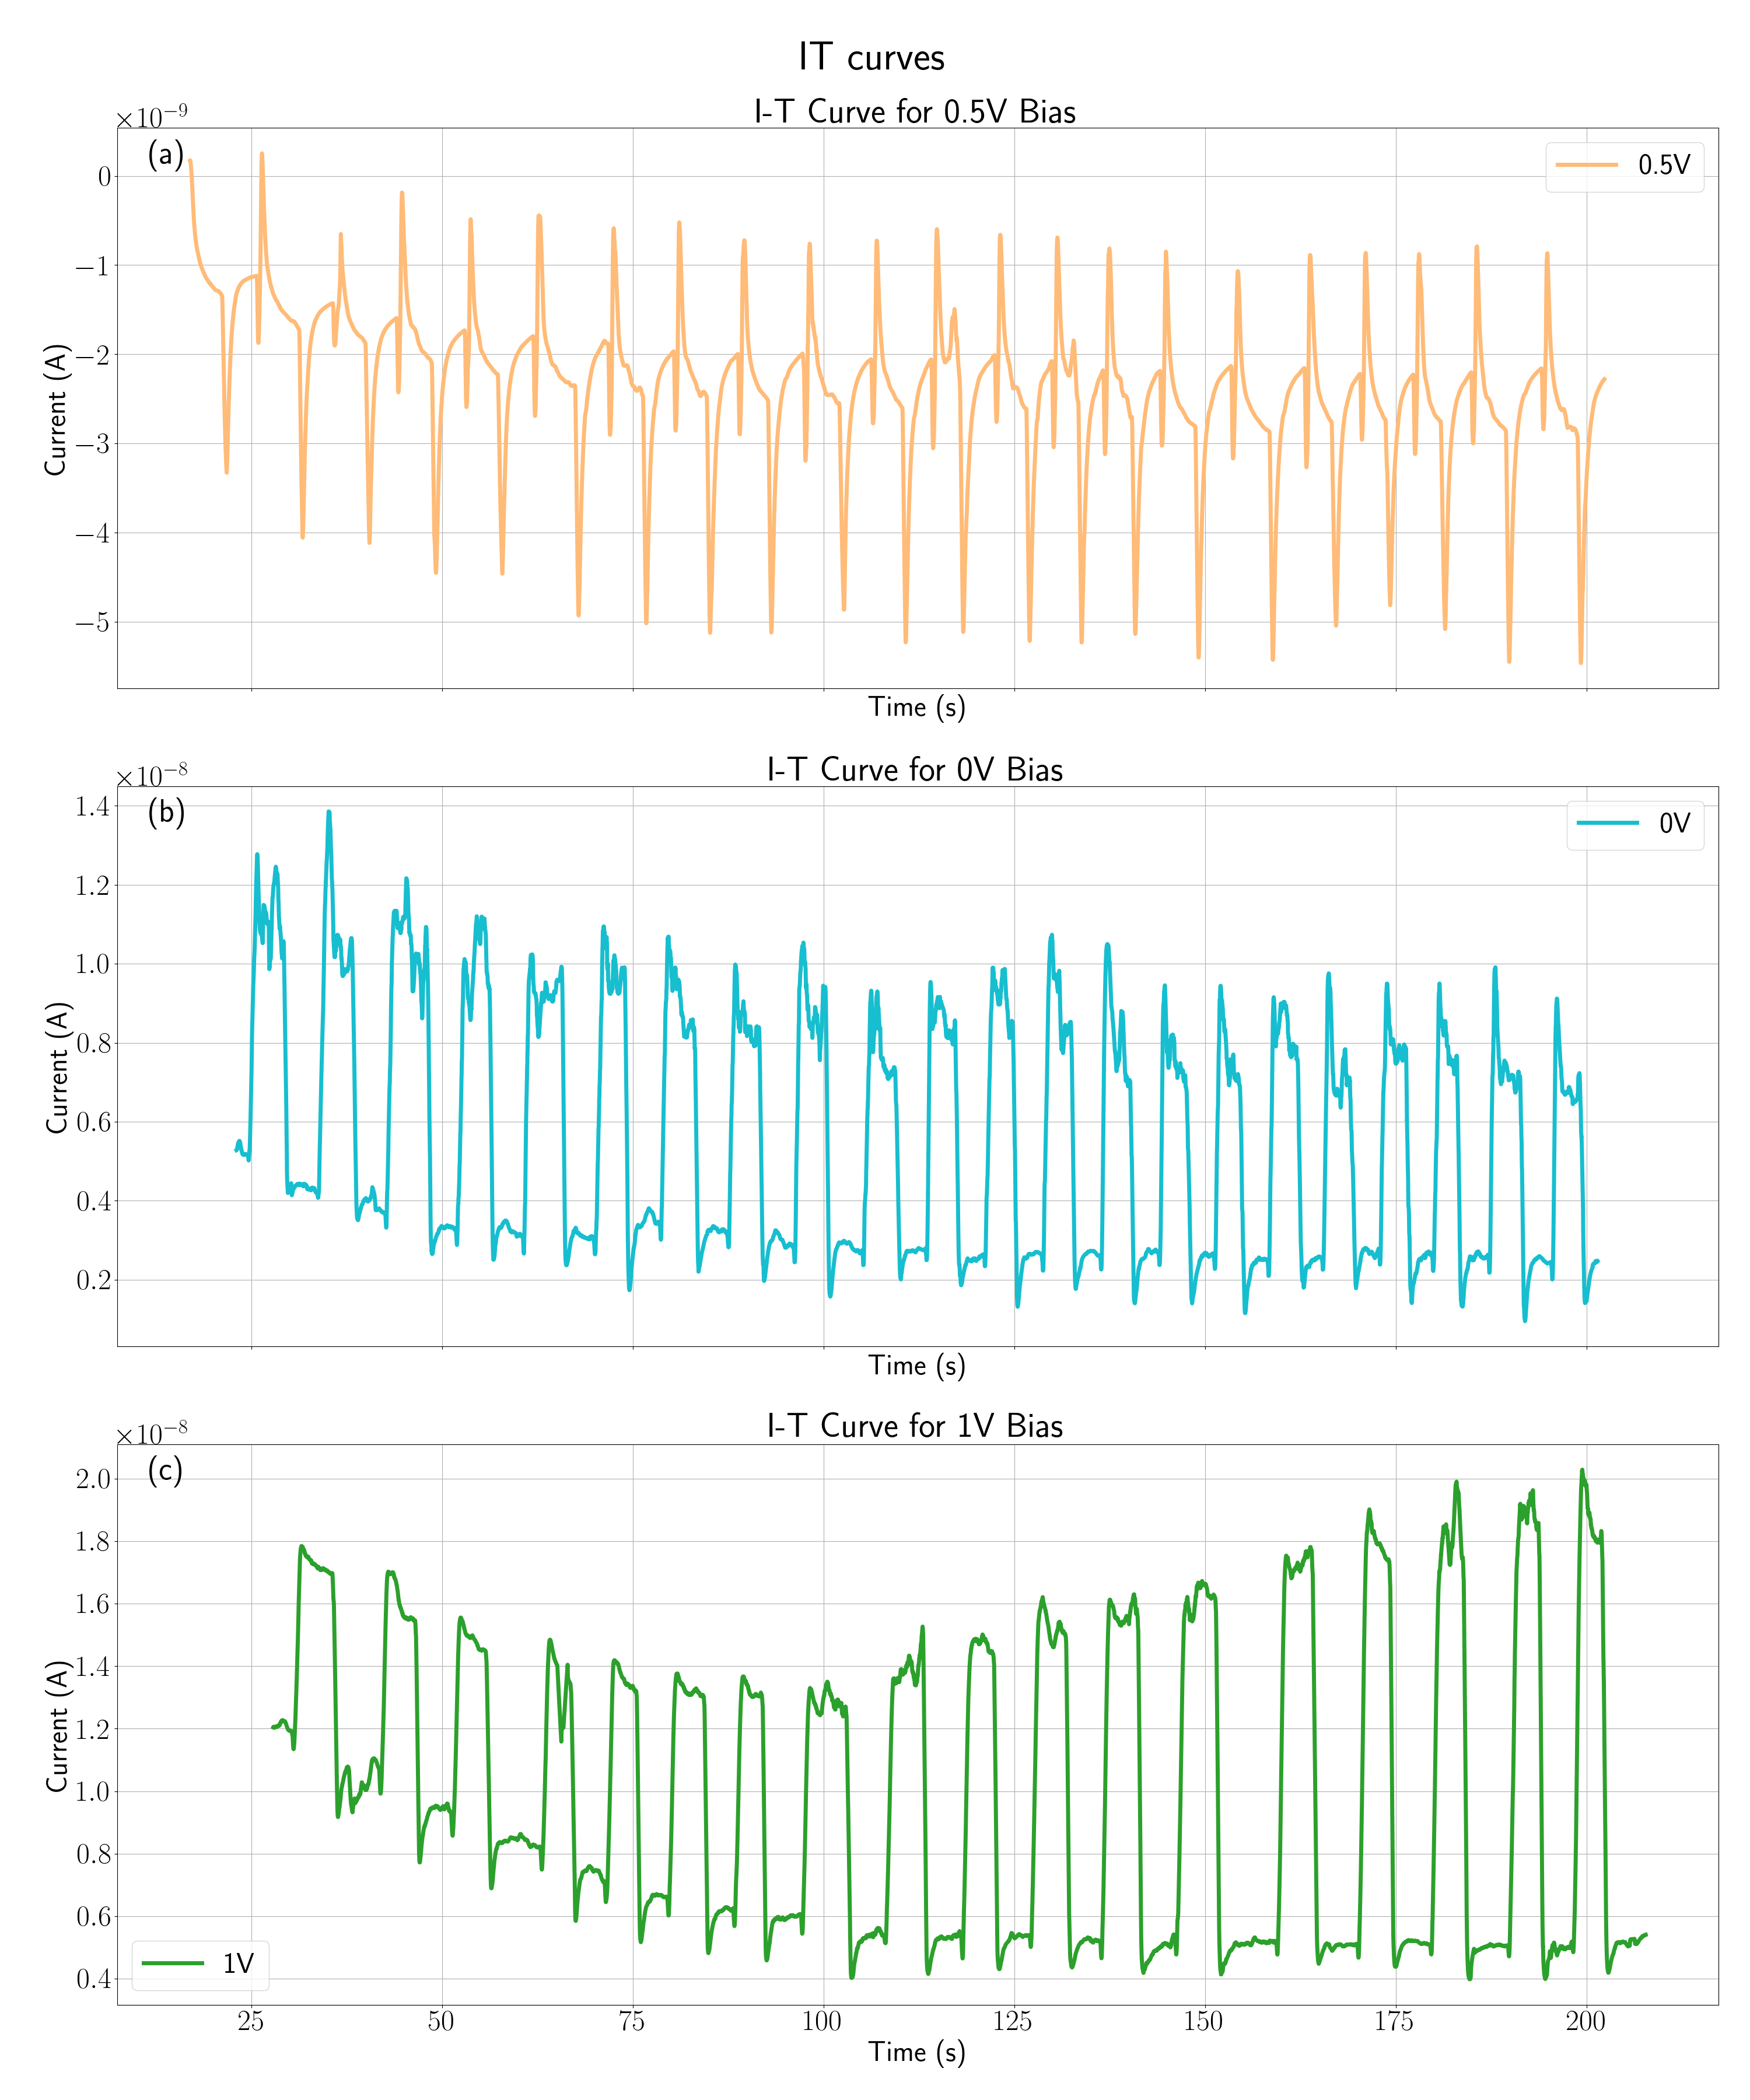
\includegraphics[width=0.7\textwidth]{results/CVD/ITs.png}
		\caption{Current Vs. Time curve of the CVD photo detector }
		\label{fig:CVDIT_individual}
	\end{figure}
	\begin{figure}[htpb]
		\centering
		\includegraphics[width=\textwidth]{results/CVD/ITs2.png}
		\caption{Overlaid Current Vs. Time curve of the CVD photo detector}
		\label{fig:CVDIT_combined}
	\end{figure}
	
	
	Key performance metrics were evaluated as functions of light intensity and bias voltage. The photocurrent ($I_{ph}$) shows a non-monotonic dependence on intensity ($0$ to $0.00175~ W/m^2$), initially increasing to $6 \times 10^{-9}$ A, then stabilizing with slight variations (Figure~\ref{fig:CVDmetrics_intensity}(a)). Responsivity decreases from $0.00025~A/W$ at low intensities to $0.000005~A/W$ at higher intensities, indicative of saturation effects (Figure~\ref{fig:CVDmetrics_intensity}(b)). Specific detectivity follows a similar trend, declining from $1200~Jones$ to $200~Jones$ (Figure~\ref{fig:CVDmetrics_intensity}(c)).
	
	Versus bias voltage ($-1$ to $1$ V), $I_{ph}$ is negative and increases in magnitude under reverse bias, reaching $-1 \times 10^{-5}$ A at $-1$ V (Figure~\ref{fig:CVDmetrics_voltage}(a)). Responsivity mirrors this, with values from $-0.03$ A/W at $-1$ V to near zero at positive biases (Figure~\ref{fig:CVDmetrics_voltage}(b)). Detectivity shows asymmetry, with higher values (up to $2 \times 10^{10}$ Jones, absolute) in reverse bias, highlighting optimal operation under reverse conditions (Figure~\ref{fig:CVDmetrics_voltage}(c)).
	
	
	
	
		
	\begin{figure}[htpb]
		\centering
		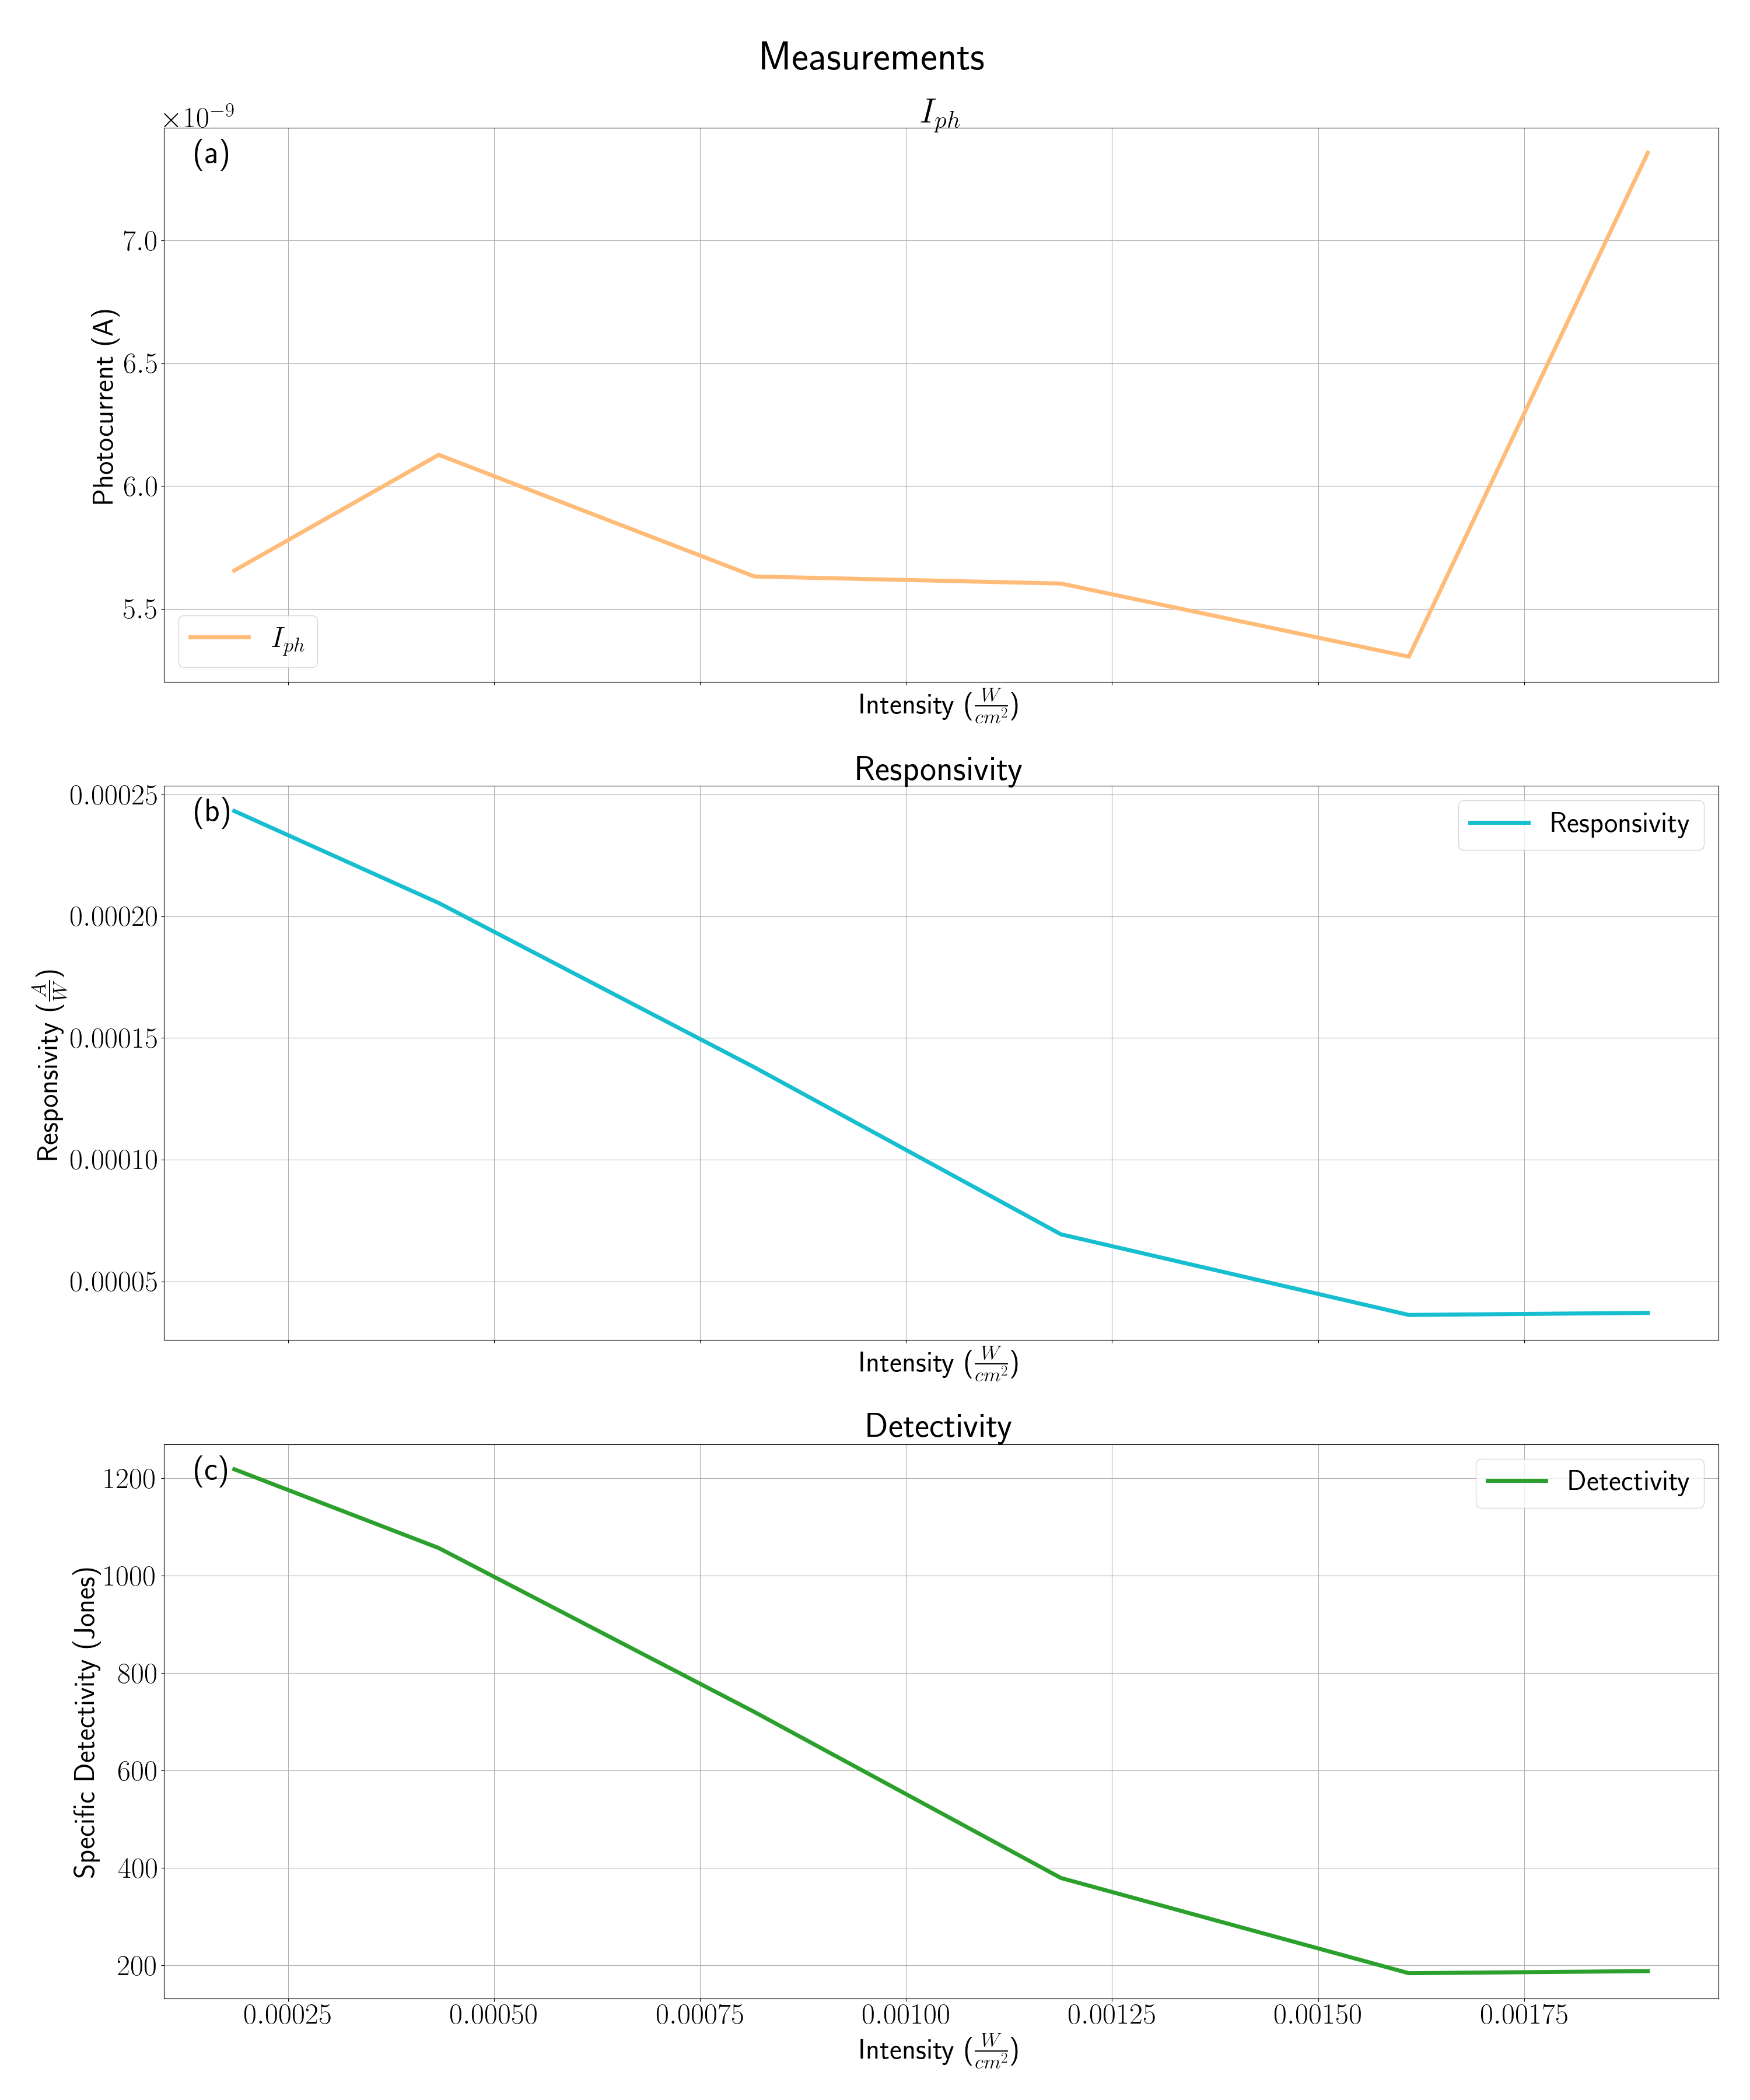
\includegraphics[width=\textwidth]{results/CVD/meas.png}
		\caption{Photo Detector measurements Vs. light intensity}
		\label{fig:CVDmetrics_intensity}
	\end{figure}
	
	\begin{figure}[htpb]
		\centering
		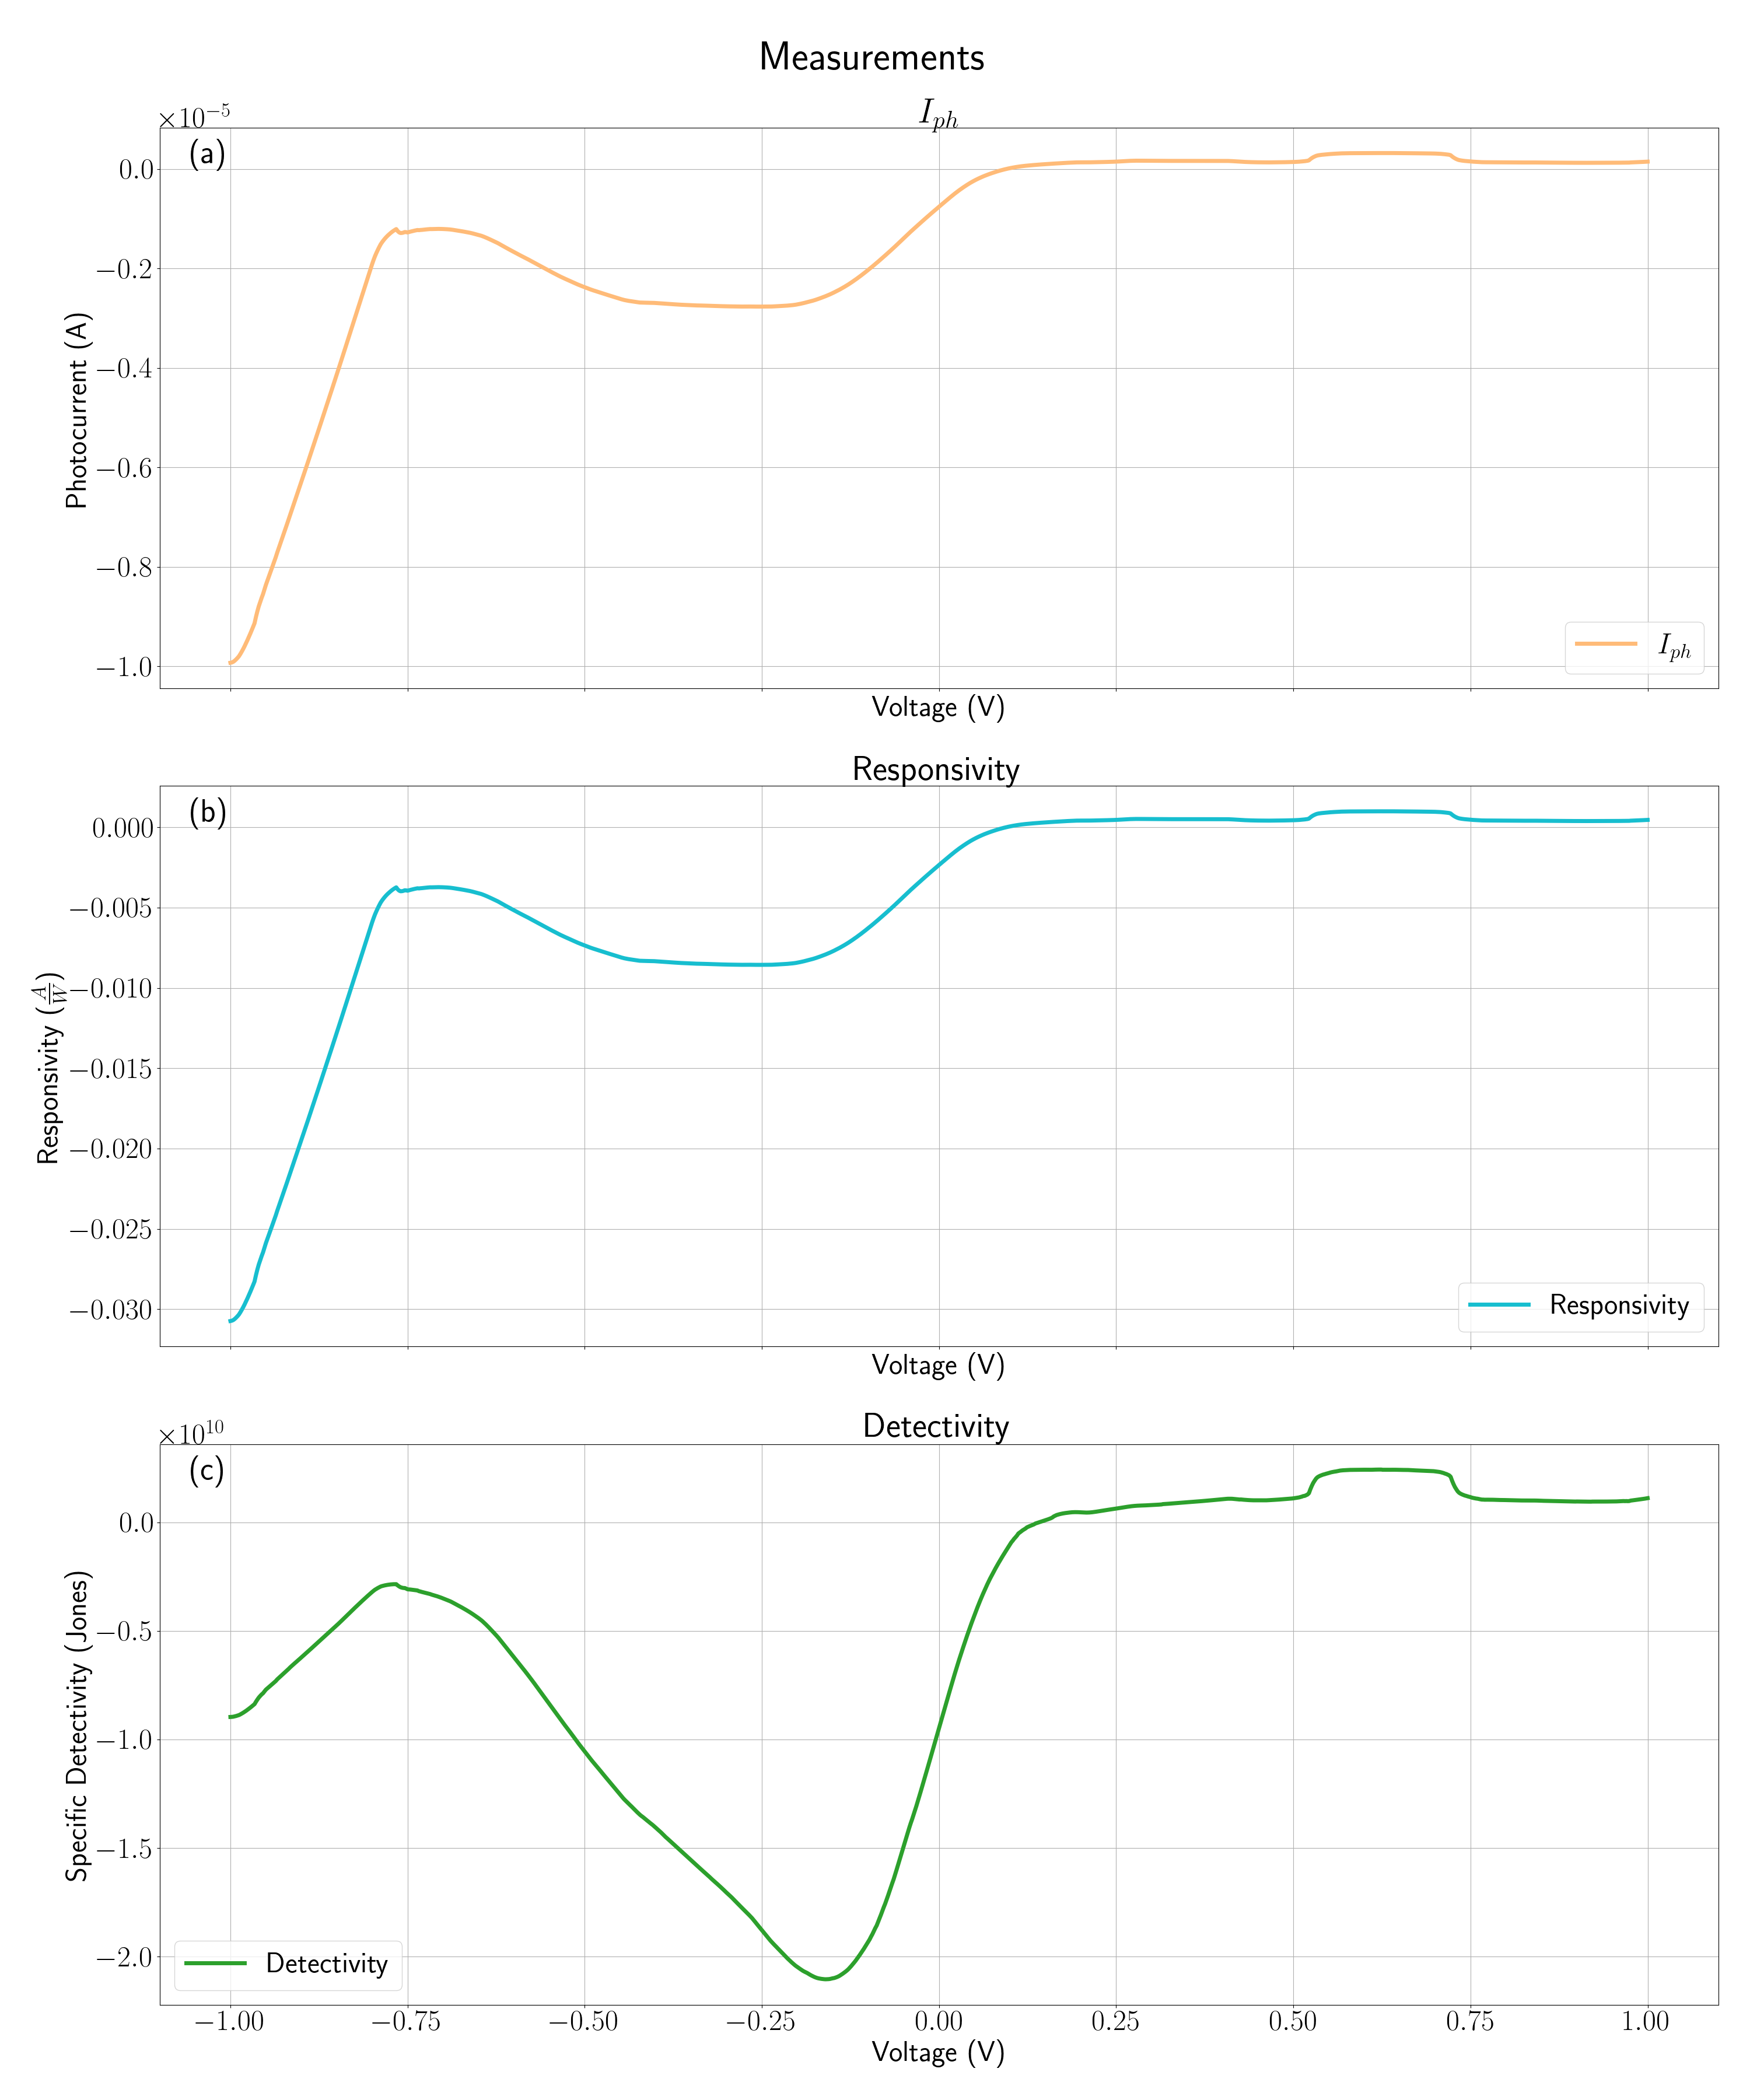
\includegraphics[width=\textwidth]{results/CVD/measurements.png}
		\caption{Photo Detector measurements Vs. bias voltage}
		\label{fig:CVDmetrics_voltage}
	\end{figure}
	
	\subsubsection{Discussion}
	
	The observed morphology confirms the efficacy of the CVD process in producing ordered nanowire arrays, which facilitate efficient charge transport along the 1D structures. The low dark current and high on/off ratio suggest minimal defect states, attributed to the vapor-solid reaction minimizing impurities. The intensity-dependent performance indicates trap-filling at low light levels, leading to high responsivity and detectivity, while saturation occurs at higher intensities due to recombination. Bias-dependent behavior underscores the role of built-in fields in self-powered operation and enhanced separation under reverse bias. Overall, these results demonstrate the potential of CVD-grown \ce{MAPbI3} nanowires for high-performance photodetectors, with opportunities for optimization in contact engineering and template design.
	
	
	
	\subsection{Comparison Between Spin-Coated and CVD-Grown Photodetectors}
	
	A comparative analysis between the spin-coated and CVD-grown perovskite nanowire photodetectors highlights the distinct advantages and limitations of each fabrication technique in terms of morphology, uniformity, alignment, and optoelectronic performance.
	
	\paragraph{Morphology and Structural Uniformity}
	
	The spin-coated \ce{MAPbBr3} nanowires exhibit highly uniform and vertically aligned arrays that precisely replicate the hexagonal pore geometry of the PAA template. The capillary-driven infiltration of the precursor solution ensures homogeneous filling and smooth nanowire surfaces, with only minor local defects attributed to incomplete infiltration or surface agglomeration. In contrast, the CVD-grown \ce{MAPbI3} nanowires display slightly lower length uniformity, with nanowire heights ranging from $2.4$ to $4~\mu$m. Although the CVD method yields high-density nanowire arrays with well-defined cylindrical morphology, occasional variations in nanowire length and thickness are observed due to nonuniform vapor distribution and local temperature gradients within the reaction zone.
	
	\paragraph{Coverage and Filling Efficiency}
	
	Spin coating provides near-complete filling of the PAA template, as confirmed by the consistent top-view SEM contrast and continuous nanowire coverage across the substrate. The wet infiltration process ensures efficient precursor penetration into nanochannels, supported by the oxygen plasma treatment that enhances wettability. The CVD method, while achieving dense vertical nanowire arrays, is more sensitive to process parameters such as precursor flux and substrate temperature. Slight nonuniformities in nanowire density across the substrate suggest that vapor-phase transport and local condensation dynamics play a stronger role in determining the coverage uniformity. Nevertheless, the overall filling efficiency of the CVD-grown arrays remains high, with array densities on the order of $10^{9}$~cm$^{-2}$.
	
	\paragraph{Alignment and Crystallinity}
	
	Both techniques produce vertically aligned nanowires guided by the PAA channel geometry; however, the degree of orientation control differs. The spin-coated nanowires exhibit exceptionally uniform vertical alignment and continuous columnar growth along the channel axis, indicating strong confinement-driven crystallization during solvent evaporation and annealing. CVD-grown nanowires also display vertical alignment but with minor deviations and occasional bundling, likely caused by vapor flow irregularities and heterogeneous nucleation within the template. The vapor-phase environment in CVD promotes the formation of large crystalline domains, while the spin-coated nanowires demonstrate comparable or superior crystallinity due to the confined solidification process and slower solvent evaporation.
	
	\paragraph{Optoelectronic Performance}
	
	The spin-coated photodetector demonstrates strong photoresponse with high responsivity ($\sim 4{-}5~\mathrm{A/W}$) and specific detectivity up to $10^{11}$~Jones at optimal bias ($5{-}7~\mathrm{V}$). However, the device exhibits stability challenges at higher biases, primarily due to ion migration and trap-mediated recombination. The CVD-based device, in comparison, exhibits more stable I–V behavior and lower dark current (on the order of $10^{-6}$~A at $-1~\mathrm{V}$), though its photocurrent enhancement ratio ($I_{\text{on}}/I_{\text{off}} \approx 3$) is more modest. This suggests that the CVD-grown nanowires favor stability and reproducibility, while the spin-coated device achieves higher sensitivity and gain under optimized bias.
	
	\paragraph{Summary}
	
	In summary, the spin-coating technique offers superior morphological uniformity, nearly complete coverage, and higher responsivity, making it advantageous for low-light detection and high-sensitivity photodetectors. Conversely, the CVD process yields nanowires with slightly lower uniformity but improved structural robustness and operational stability, suitable for applications requiring long-term reliability. The choice between the two fabrication routes thus depends on the intended device application—whether the focus is on high sensitivity or operational endurance.
	
	
	\newpage
	\bibliographystyle{IEEEtran}
	\bibliography{ref.bib}
\end{document}